
\begin{DoxyItemize}
\item \hyperlink{mathfunctions_acos}{A\-C\-O\-S Inverse Trigonometric Arccosine Function}  
\item \hyperlink{mathfunctions_acosd}{A\-C\-O\-S\-D Inverse Cosine Degrees Function}  
\item \hyperlink{mathfunctions_acosh}{A\-C\-O\-S\-H Inverse Hyperbolic Cosine Function}  
\item \hyperlink{mathfunctions_acot}{A\-C\-O\-T Inverse Cotangent Function}  
\item \hyperlink{mathfunctions_acotd}{A\-C\-O\-T\-D Inverse Cotangent Degrees Function}  
\item \hyperlink{mathfunctions_acoth}{A\-C\-O\-T\-H Inverse Hyperbolic Cotangent Function}  
\item \hyperlink{mathfunctions_acsc}{A\-C\-S\-C Inverse Cosecant Function}  
\item \hyperlink{mathfunctions_acscd}{A\-C\-S\-C\-D Inverse Cosecant Degrees Function}  
\item \hyperlink{mathfunctions_acsch}{A\-C\-S\-C\-H Inverse Hyperbolic Cosecant Function}  
\item \hyperlink{mathfunctions_angle}{A\-N\-G\-L\-E Phase Angle Function}  
\item \hyperlink{mathfunctions_asec}{A\-S\-E\-C Inverse Secant Function}  
\item \hyperlink{mathfunctions_asecd}{A\-S\-E\-C\-D Inverse Secant Degrees Function}  
\item \hyperlink{mathfunctions_asech}{A\-S\-E\-C\-H Inverse Hyperbolic Secant Function}  
\item \hyperlink{mathfunctions_asin}{A\-S\-I\-N Inverse Trigonometric Arcsine Function}  
\item \hyperlink{mathfunctions_asind}{A\-S\-I\-N\-D Inverse Sine Degrees Function}  
\item \hyperlink{mathfunctions_asinh}{A\-S\-I\-N\-H Inverse Hyperbolic Sine Function}  
\item \hyperlink{mathfunctions_atan}{A\-T\-A\-N Inverse Trigonometric Arctangent Function}  
\item \hyperlink{mathfunctions_atan2}{A\-T\-A\-N2 Inverse Trigonometric 4-\/\-Quadrant Arctangent Function}  
\item \hyperlink{mathfunctions_atand}{A\-T\-A\-N\-D Inverse Tangent Degrees Function}  
\item \hyperlink{mathfunctions_atanh}{A\-T\-A\-N\-H Inverse Hyperbolic Tangent Function}  
\item \hyperlink{mathfunctions_betainc}{B\-E\-T\-A\-I\-N\-C Incomplete Beta Function}  
\item \hyperlink{mathfunctions_cos}{C\-O\-S Trigonometric Cosine Function}  
\item \hyperlink{mathfunctions_cosd}{C\-O\-S\-D Cosine Degrees Function}  
\item \hyperlink{mathfunctions_cosh}{C\-O\-S\-H Hyperbolic Cosine Function}  
\item \hyperlink{mathfunctions_cot}{C\-O\-T Trigonometric Cotangent Function}  
\item \hyperlink{mathfunctions_cotd}{C\-O\-T\-D Cotangent Degrees Function}  
\item \hyperlink{mathfunctions_coth}{C\-O\-T\-H Hyperbolic Cotangent Function}  
\item \hyperlink{mathfunctions_cross}{C\-R\-O\-S\-S Cross Product of Two Vectors}  
\item \hyperlink{mathfunctions_csc}{C\-S\-C Trigonometric Cosecant Function}  
\item \hyperlink{mathfunctions_cscd}{C\-S\-C\-D Cosecant Degrees Function}  
\item \hyperlink{mathfunctions_csch}{C\-S\-C\-H Hyperbolic Cosecant Function}  
\item \hyperlink{mathfunctions_deg2rad}{D\-E\-G2\-R\-A\-D Convert From Degrees To Radians}  
\item \hyperlink{mathfunctions_erf}{E\-R\-F Error Function}  
\item \hyperlink{mathfunctions_erfc}{E\-R\-F\-C Complimentary Error Function}  
\item \hyperlink{mathfunctions_erfinv}{E\-R\-F\-I\-N\-V Inverse Error Function}  
\item \hyperlink{mathfunctions_exp}{E\-X\-P Exponential Function}  
\item \hyperlink{mathfunctions_expm1}{E\-X\-P\-M1 Exponential Minus One Function}  
\item \hyperlink{mathfunctions_fix}{F\-I\-X Round Towards Zero}  
\item \hyperlink{mathfunctions_gamma}{G\-A\-M\-M\-A Gamma Function}  
\item \hyperlink{mathfunctions_gammaln}{G\-A\-M\-M\-A\-L\-N Log Gamma Function}  
\item \hyperlink{mathfunctions_idiv}{I\-D\-I\-V Integer Division Operation}  
\item \hyperlink{mathfunctions_legendre}{L\-E\-G\-E\-N\-D\-R\-E Associated Legendre Polynomial}  
\item \hyperlink{mathfunctions_log}{L\-O\-G Natural Logarithm Function}  
\item \hyperlink{mathfunctions_log10}{L\-O\-G10 Base-\/10 Logarithm Function}  
\item \hyperlink{mathfunctions_log1p}{L\-O\-G1\-P Natural Logarithm of 1+\-P Function}  
\item \hyperlink{mathfunctions_log2}{L\-O\-G2 Base-\/2 Logarithm Function}  
\item \hyperlink{mathfunctions_mod}{M\-O\-D Modulus Operation}  
\item \hyperlink{mathfunctions_mpower}{M\-P\-O\-W\-E\-R Matrix Power Function}  
\item \hyperlink{mathfunctions_power}{P\-O\-W\-E\-R Element-\/wise Power Function}  
\item \hyperlink{mathfunctions_rad2deg}{R\-A\-D2\-D\-E\-G Radians To Degrees Conversion Function}  
\item \hyperlink{mathfunctions_rem}{R\-E\-M Remainder After Division}  
\item \hyperlink{mathfunctions_sec}{S\-E\-C Trigonometric Secant Function}  
\item \hyperlink{mathfunctions_secd}{S\-E\-C\-D Secant Degrees Function}  
\item \hyperlink{mathfunctions_sech}{S\-E\-C\-H Hyperbolic Secant Function}  
\item \hyperlink{mathfunctions_sin}{S\-I\-N Trigonometric Sine Function}  
\item \hyperlink{mathfunctions_sind}{S\-I\-N\-D Sine Degrees Function}  
\item \hyperlink{mathfunctions_sinh}{S\-I\-N\-H Hyperbolic Sine Function}  
\item \hyperlink{mathfunctions_sqrt}{S\-Q\-R\-T Square Root of an Array}  
\item \hyperlink{mathfunctions_tan}{T\-A\-N Trigonometric Tangent Function}  
\item \hyperlink{mathfunctions_tand}{T\-A\-N\-D Tangent Degrees Function}  
\item \hyperlink{mathfunctions_tanh}{T\-A\-N\-H Hyperbolic Tangent Function}  
\end{DoxyItemize}\hypertarget{mathfunctions_acos}{}\section{A\-C\-O\-S Inverse Trigonometric Arccosine Function}\label{mathfunctions_acos}
Section\-: \hyperlink{sec_mathfunctions}{Mathematical Functions} \hypertarget{vtkwidgets_vtkxyplotwidget_Usage}{}\subsection{Usage}\label{vtkwidgets_vtkxyplotwidget_Usage}
Computes the {\ttfamily acos} function for its argument. The general syntax for its use is \begin{DoxyVerb}  y = acos(x)
\end{DoxyVerb}
 where {\ttfamily x} is an {\ttfamily n}-\/dimensional array of numerical type. Integer types are promoted to the {\ttfamily double} type prior to calculation of the {\ttfamily acos} function. Output {\ttfamily y} is of the same size and type as the input {\ttfamily x}, (unless {\ttfamily x} is an integer, in which case {\ttfamily y} is a {\ttfamily double} type). \hypertarget{transforms_svd_Function}{}\subsection{Internals}\label{transforms_svd_Function}
Mathematically, the {\ttfamily acos} function is defined for all arguments {\ttfamily x} as \[ \mathrm{acos} x \equiv \frac{pi}{2} + i \log \left(i x + \sqrt{1-x^2}\right). \] For real valued variables {\ttfamily x} in the range {\ttfamily \mbox{[}-\/1,1\mbox{]}}, the function is computed directly using the standard C library's numerical {\ttfamily acos} function. For both real and complex arguments {\ttfamily x}, note that generally \[ \mathrm{acos}(\cos(x)) \neq x, \] \hypertarget{variables_struct_Example}{}\subsection{Example}\label{variables_struct_Example}
The following code demonstates the {\ttfamily acos} function over the range {\ttfamily \mbox{[}-\/1,1\mbox{]}}.


\begin{DoxyVerbInclude}
--> t = linspace(-1,1);
--> plot(t,acos(t))
\end{DoxyVerbInclude}


 
\begin{DoxyImage}
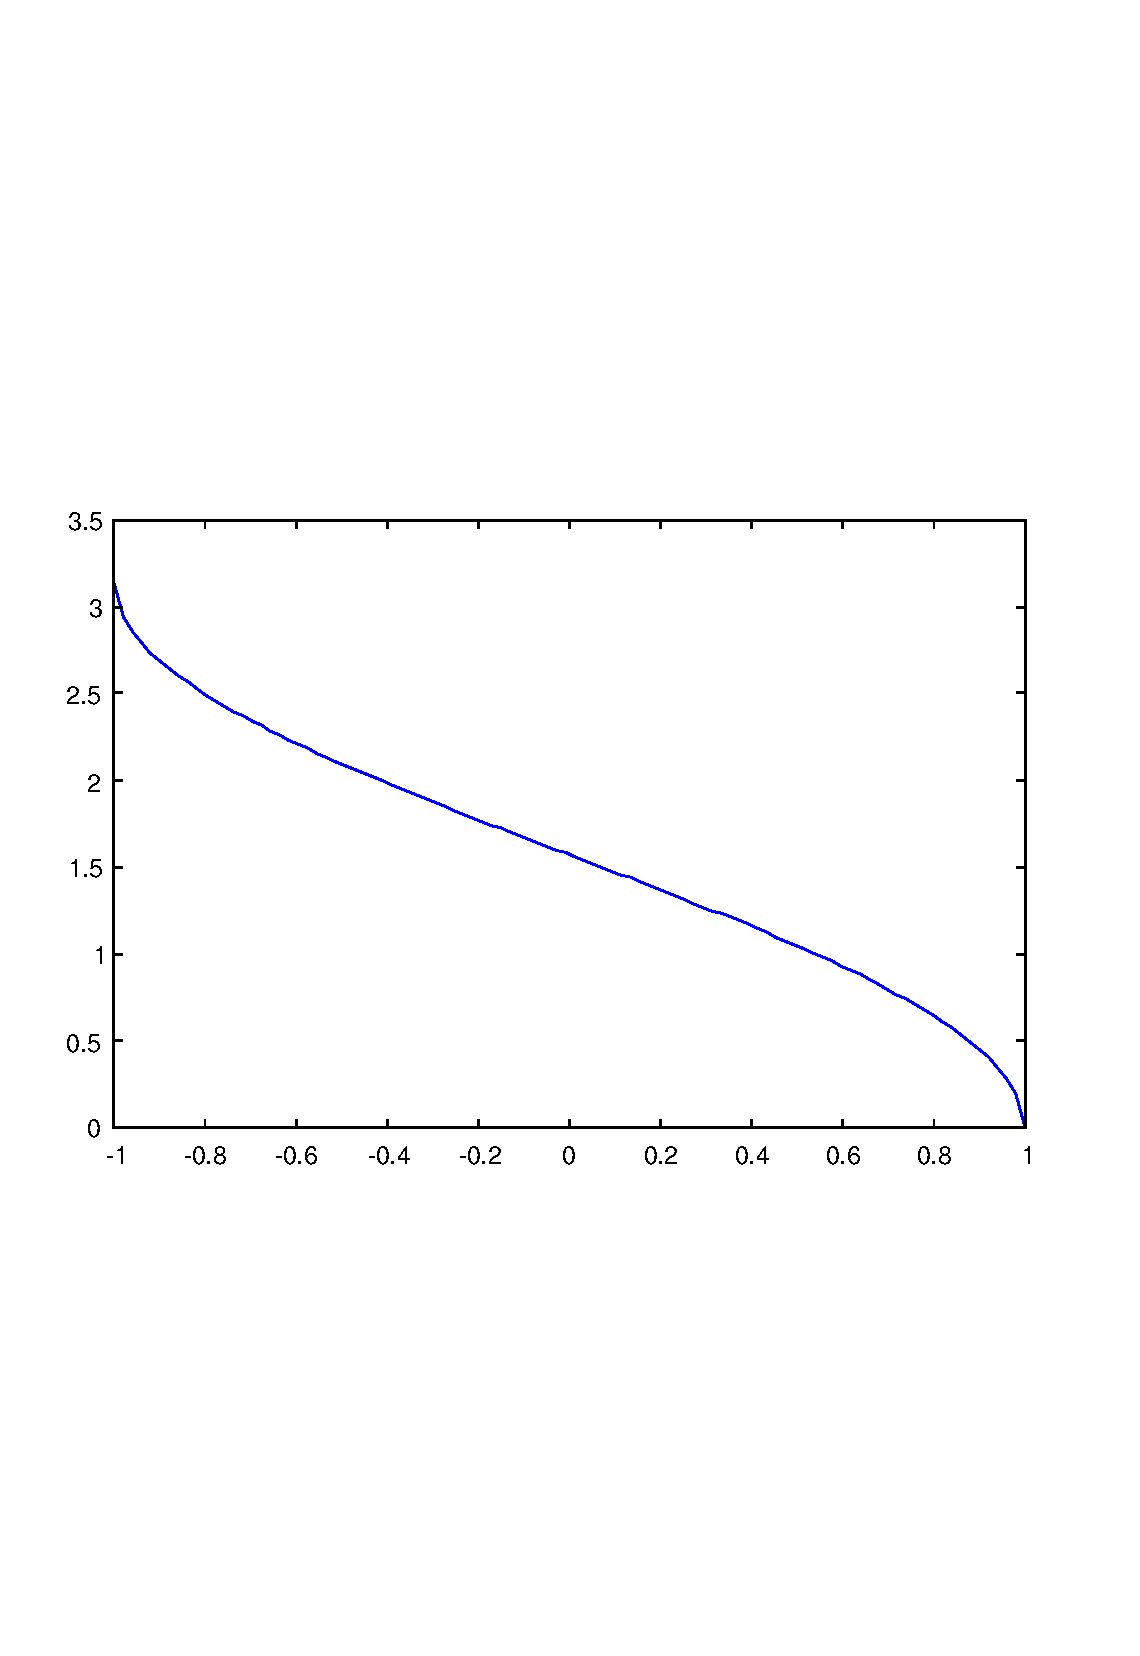
\includegraphics[width=12cm]{acosplot}
\caption{acosplot}
\end{DoxyImage}
 \hypertarget{mathfunctions_acosd}{}\section{A\-C\-O\-S\-D Inverse Cosine Degrees Function}\label{mathfunctions_acosd}
Section\-: \hyperlink{sec_mathfunctions}{Mathematical Functions} \hypertarget{vtkwidgets_vtkxyplotwidget_Usage}{}\subsection{Usage}\label{vtkwidgets_vtkxyplotwidget_Usage}
Computes the inverse cosine of the argument, but returns the argument in degrees instead of radians (as is the case for {\ttfamily acos}. The syntax for its use is \begin{DoxyVerb}   y = acosd(x)
\end{DoxyVerb}
 \hypertarget{variables_matrix_Examples}{}\subsection{Examples}\label{variables_matrix_Examples}
The inverse cosine of {\ttfamily sqrt(2)/2} should be 45 degrees\-:


\begin{DoxyVerbInclude}
--> acosd(sqrt(2)/2)

ans = 
  45.0000 +  0.0000i 
\end{DoxyVerbInclude}


and the inverse cosine of {\ttfamily 0.\-5} should be 60 degrees\-:


\begin{DoxyVerbInclude}
--> acosd(0.5)

ans = 
  60.0000 +  0.0000i 
\end{DoxyVerbInclude}
 \hypertarget{mathfunctions_acosh}{}\section{A\-C\-O\-S\-H Inverse Hyperbolic Cosine Function}\label{mathfunctions_acosh}
Section\-: \hyperlink{sec_mathfunctions}{Mathematical Functions} \hypertarget{vtkwidgets_vtkxyplotwidget_Usage}{}\subsection{Usage}\label{vtkwidgets_vtkxyplotwidget_Usage}
Computes the inverse hyperbolic cosine of its argument. The general syntax for its use is \begin{DoxyVerb}  y = acosh(x)
\end{DoxyVerb}
 where {\ttfamily x} is an {\ttfamily n}-\/dimensional array of numerical type. \hypertarget{transforms_svd_Function}{}\subsection{Internals}\label{transforms_svd_Function}
The {\ttfamily acosh} function is computed from the formula \[ \cosh^{-1}(x) = \log\left(x + (x^2 - 1)^0.5\right) \] where the {\ttfamily log} (and square root) is taken in its most general sense. \hypertarget{variables_matrix_Examples}{}\subsection{Examples}\label{variables_matrix_Examples}
Here is a simple plot of the inverse hyperbolic cosine function


\begin{DoxyVerbInclude}
--> x = linspace(1,pi);
--> plot(x,acosh(x)); grid('on');
\end{DoxyVerbInclude}


 
\begin{DoxyImage}
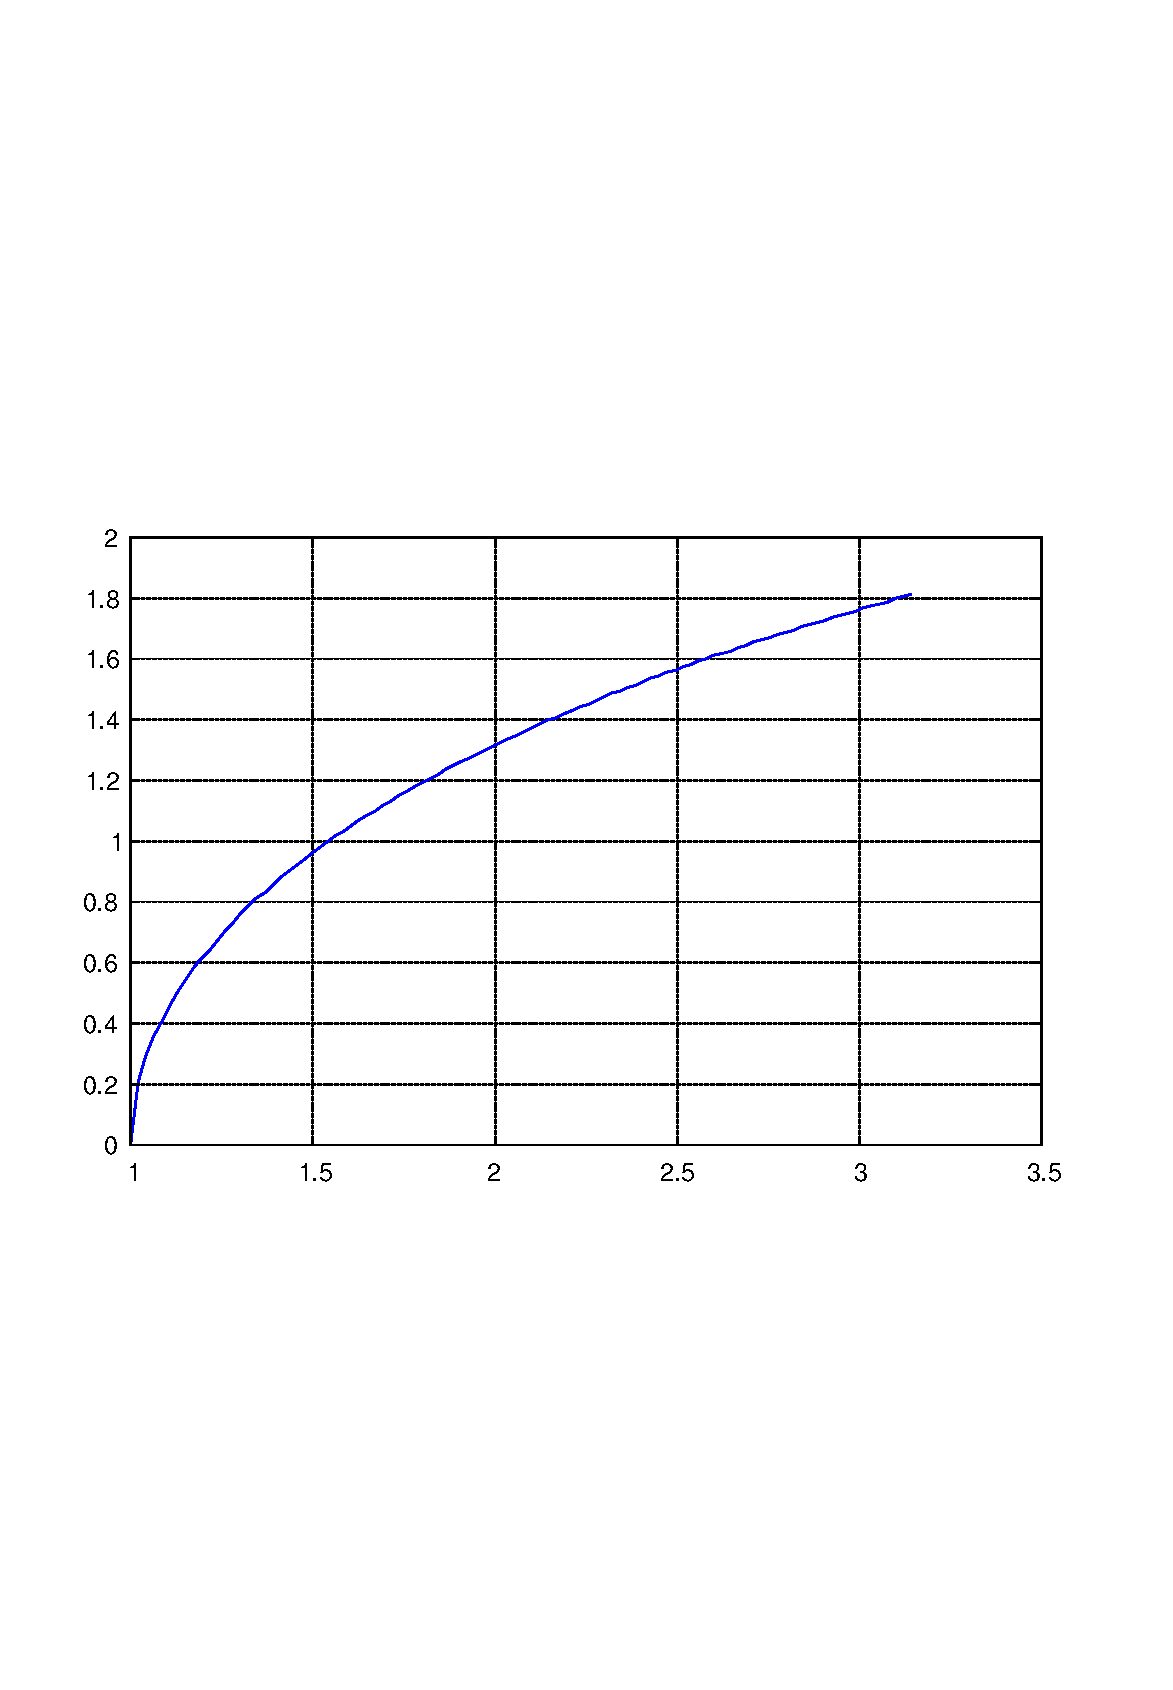
\includegraphics[width=12cm]{acoshplot}
\caption{acoshplot}
\end{DoxyImage}
 \hypertarget{mathfunctions_acot}{}\section{A\-C\-O\-T Inverse Cotangent Function}\label{mathfunctions_acot}
Section\-: \hyperlink{sec_mathfunctions}{Mathematical Functions} \hypertarget{vtkwidgets_vtkxyplotwidget_Usage}{}\subsection{Usage}\label{vtkwidgets_vtkxyplotwidget_Usage}
Computes the inverse cotangent of its argument. The general syntax for its use is \begin{DoxyVerb}  y = acot(x)
\end{DoxyVerb}
 where {\ttfamily x} is an {\ttfamily n}-\/dimensional array of numerical type. \hypertarget{transforms_svd_Function}{}\subsection{Internals}\label{transforms_svd_Function}
The {\ttfamily acot} function is computed from the formula \[ \cot^{-1}(x) = \tan^{-1}\left(\frac{1}{x}\right) \] \hypertarget{variables_matrix_Examples}{}\subsection{Examples}\label{variables_matrix_Examples}
Here is a simple plot of the inverse cotangent function


\begin{DoxyVerbInclude}
--> x1 = -2*pi:pi/30:-0.1;
--> x2 = 0.1:pi/30:2*pi;
--> plot(x1,acot(x1),x2,acot(x2)); grid('on');
\end{DoxyVerbInclude}


 
\begin{DoxyImage}
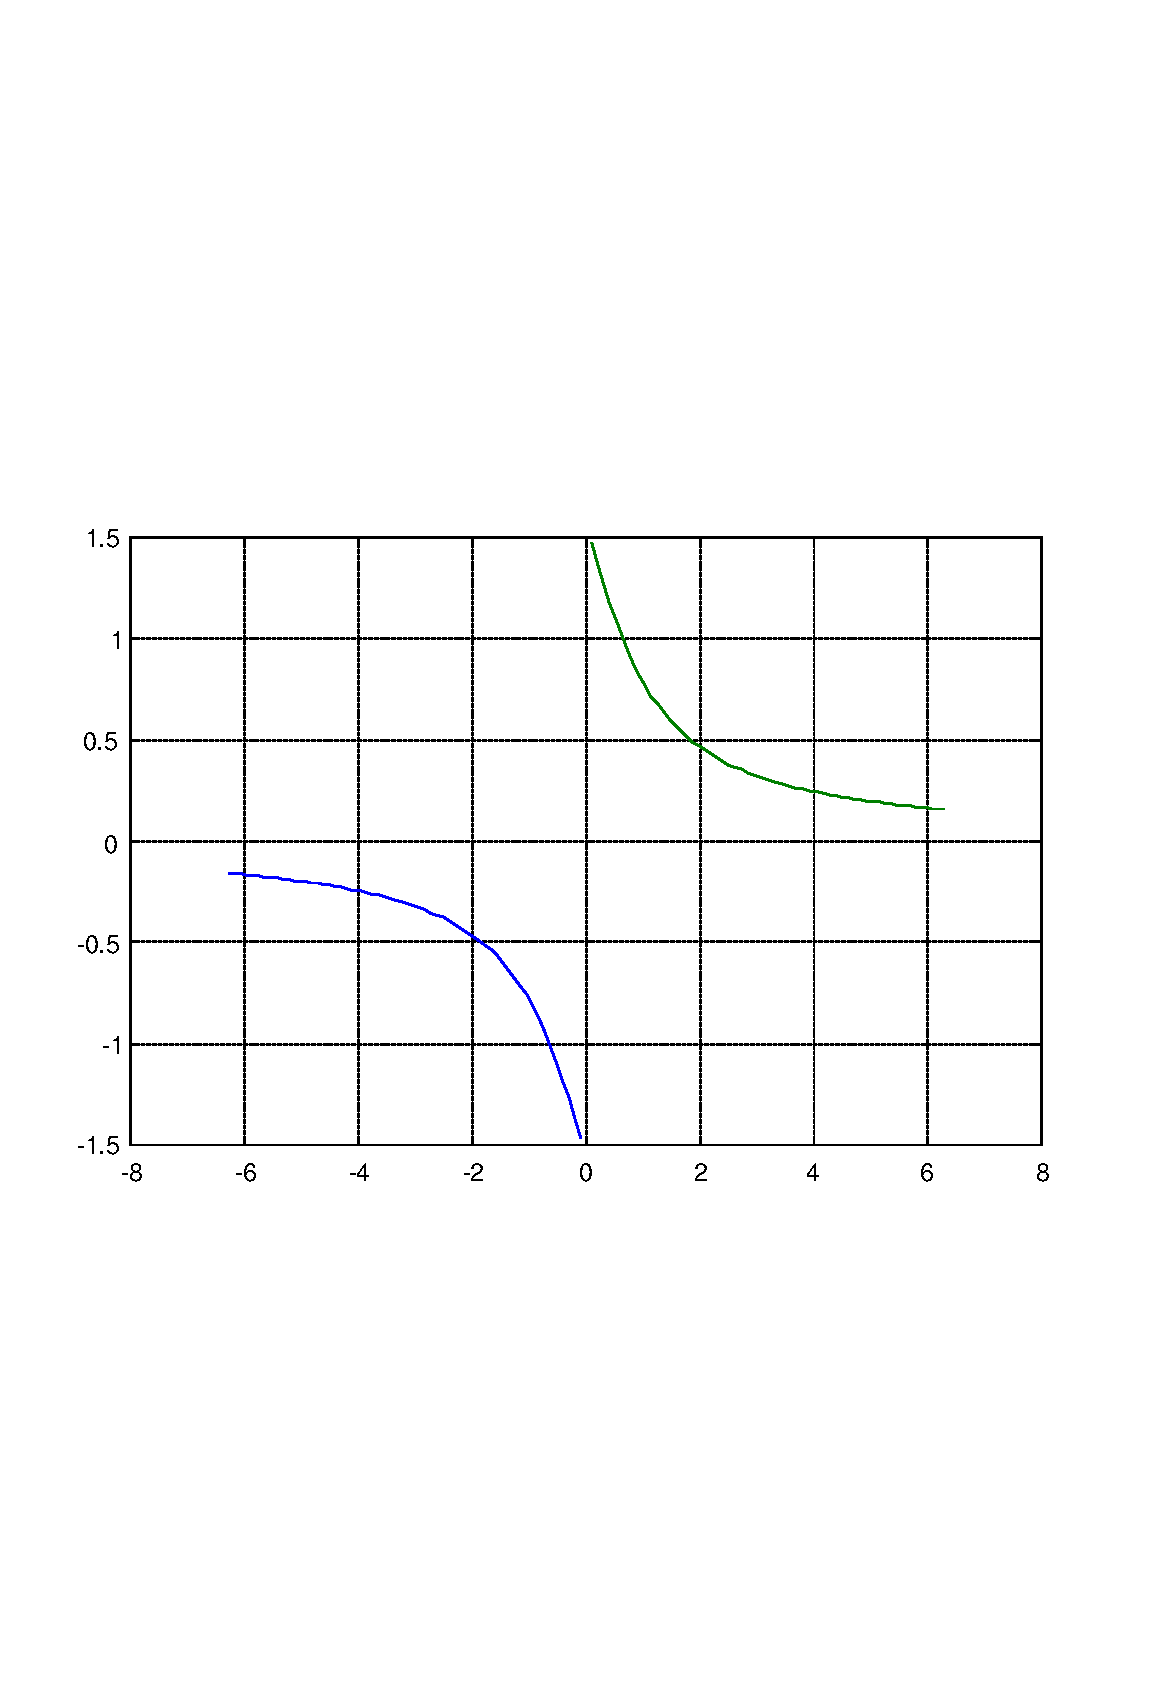
\includegraphics[width=12cm]{acotplot}
\caption{acotplot}
\end{DoxyImage}
 \hypertarget{mathfunctions_acotd}{}\section{A\-C\-O\-T\-D Inverse Cotangent Degrees Function}\label{mathfunctions_acotd}
Section\-: \hyperlink{sec_mathfunctions}{Mathematical Functions} \hypertarget{vtkwidgets_vtkxyplotwidget_Usage}{}\subsection{Usage}\label{vtkwidgets_vtkxyplotwidget_Usage}
Computes the inverse cotangent of its argument in degrees. The general syntax for its use is \begin{DoxyVerb}  y = acotd(x)
\end{DoxyVerb}
 where {\ttfamily x} is an {\ttfamily n}-\/dimensional array of numerical type. \hypertarget{mathfunctions_acoth}{}\section{A\-C\-O\-T\-H Inverse Hyperbolic Cotangent Function}\label{mathfunctions_acoth}
Section\-: \hyperlink{sec_mathfunctions}{Mathematical Functions} \hypertarget{vtkwidgets_vtkxyplotwidget_Usage}{}\subsection{Usage}\label{vtkwidgets_vtkxyplotwidget_Usage}
Computes the inverse hyperbolic cotangent of its argument. The general syntax for its use is \begin{DoxyVerb}  y = acoth(x)
\end{DoxyVerb}
 where {\ttfamily x} is an {\ttfamily n}-\/dimensional array of numerical type. \hypertarget{transforms_svd_Function}{}\subsection{Internals}\label{transforms_svd_Function}
The {\ttfamily acoth} function is computed from the formula \[ \coth^{-1}(x) = \tanh^{-1}\left(\frac{1}{x}\right) \] \hypertarget{variables_matrix_Examples}{}\subsection{Examples}\label{variables_matrix_Examples}
Here is a simple plot of the inverse hyperbolic cotangent function


\begin{DoxyVerbInclude}
--> x = linspace(1,pi);
--> plot(x,acoth(x)); grid('on');
\end{DoxyVerbInclude}


 
\begin{DoxyImage}
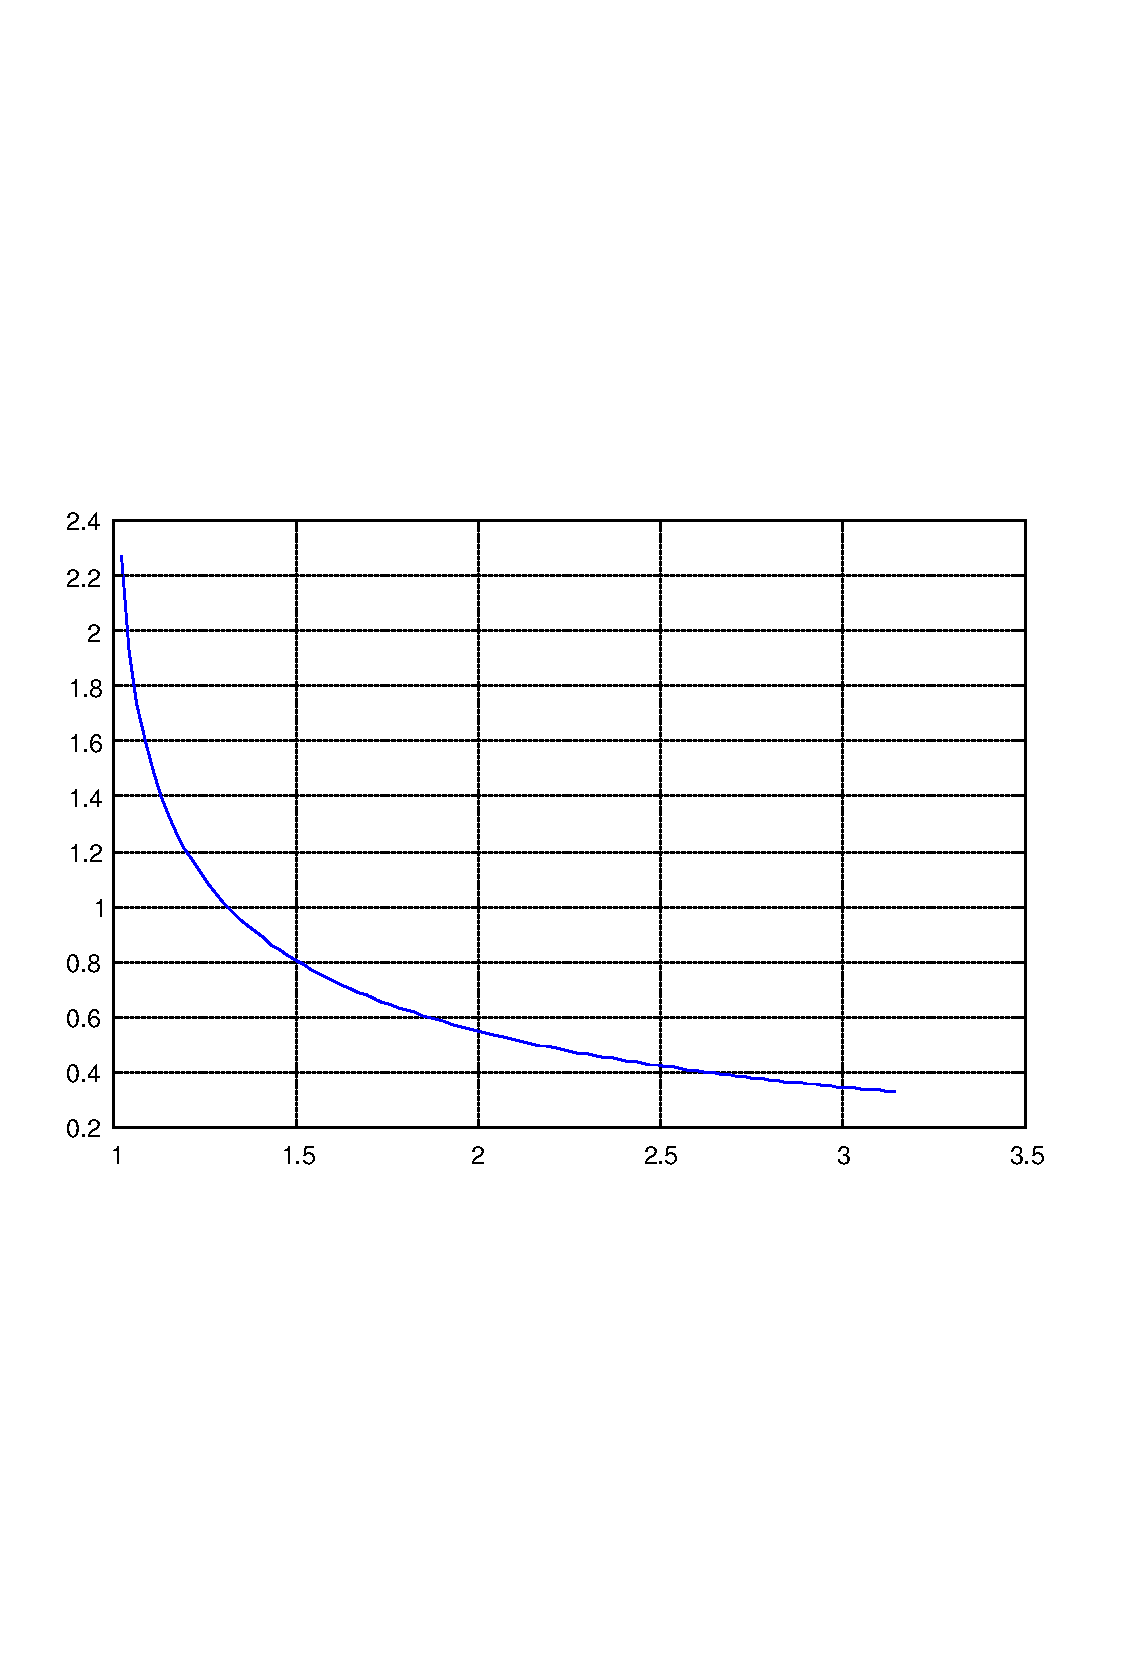
\includegraphics[width=12cm]{acothplot}
\caption{acothplot}
\end{DoxyImage}
 \hypertarget{mathfunctions_acsc}{}\section{A\-C\-S\-C Inverse Cosecant Function}\label{mathfunctions_acsc}
Section\-: \hyperlink{sec_mathfunctions}{Mathematical Functions} \hypertarget{vtkwidgets_vtkxyplotwidget_Usage}{}\subsection{Usage}\label{vtkwidgets_vtkxyplotwidget_Usage}
Computes the inverse cosecant of its argument. The general syntax for its use is \begin{DoxyVerb}  y = acsc(x)
\end{DoxyVerb}
 where {\ttfamily x} is an {\ttfamily n}-\/dimensional array of numerical type. \hypertarget{transforms_svd_Function}{}\subsection{Internals}\label{transforms_svd_Function}
The {\ttfamily acosh} function is computed from the formula \[ \csc^{-1}(x) = \sin^{-1}\left(\frac{1}{x}\right) \] \hypertarget{variables_matrix_Examples}{}\subsection{Examples}\label{variables_matrix_Examples}
Here is a simple plot of the inverse cosecant function


\begin{DoxyVerbInclude}
--> x1 = -10:.01:-1.01;
--> x2 = 1.01:.01:10;
--> plot(x1,acsc(x1),x2,acsc(x2)); grid('on');
\end{DoxyVerbInclude}


 
\begin{DoxyImage}
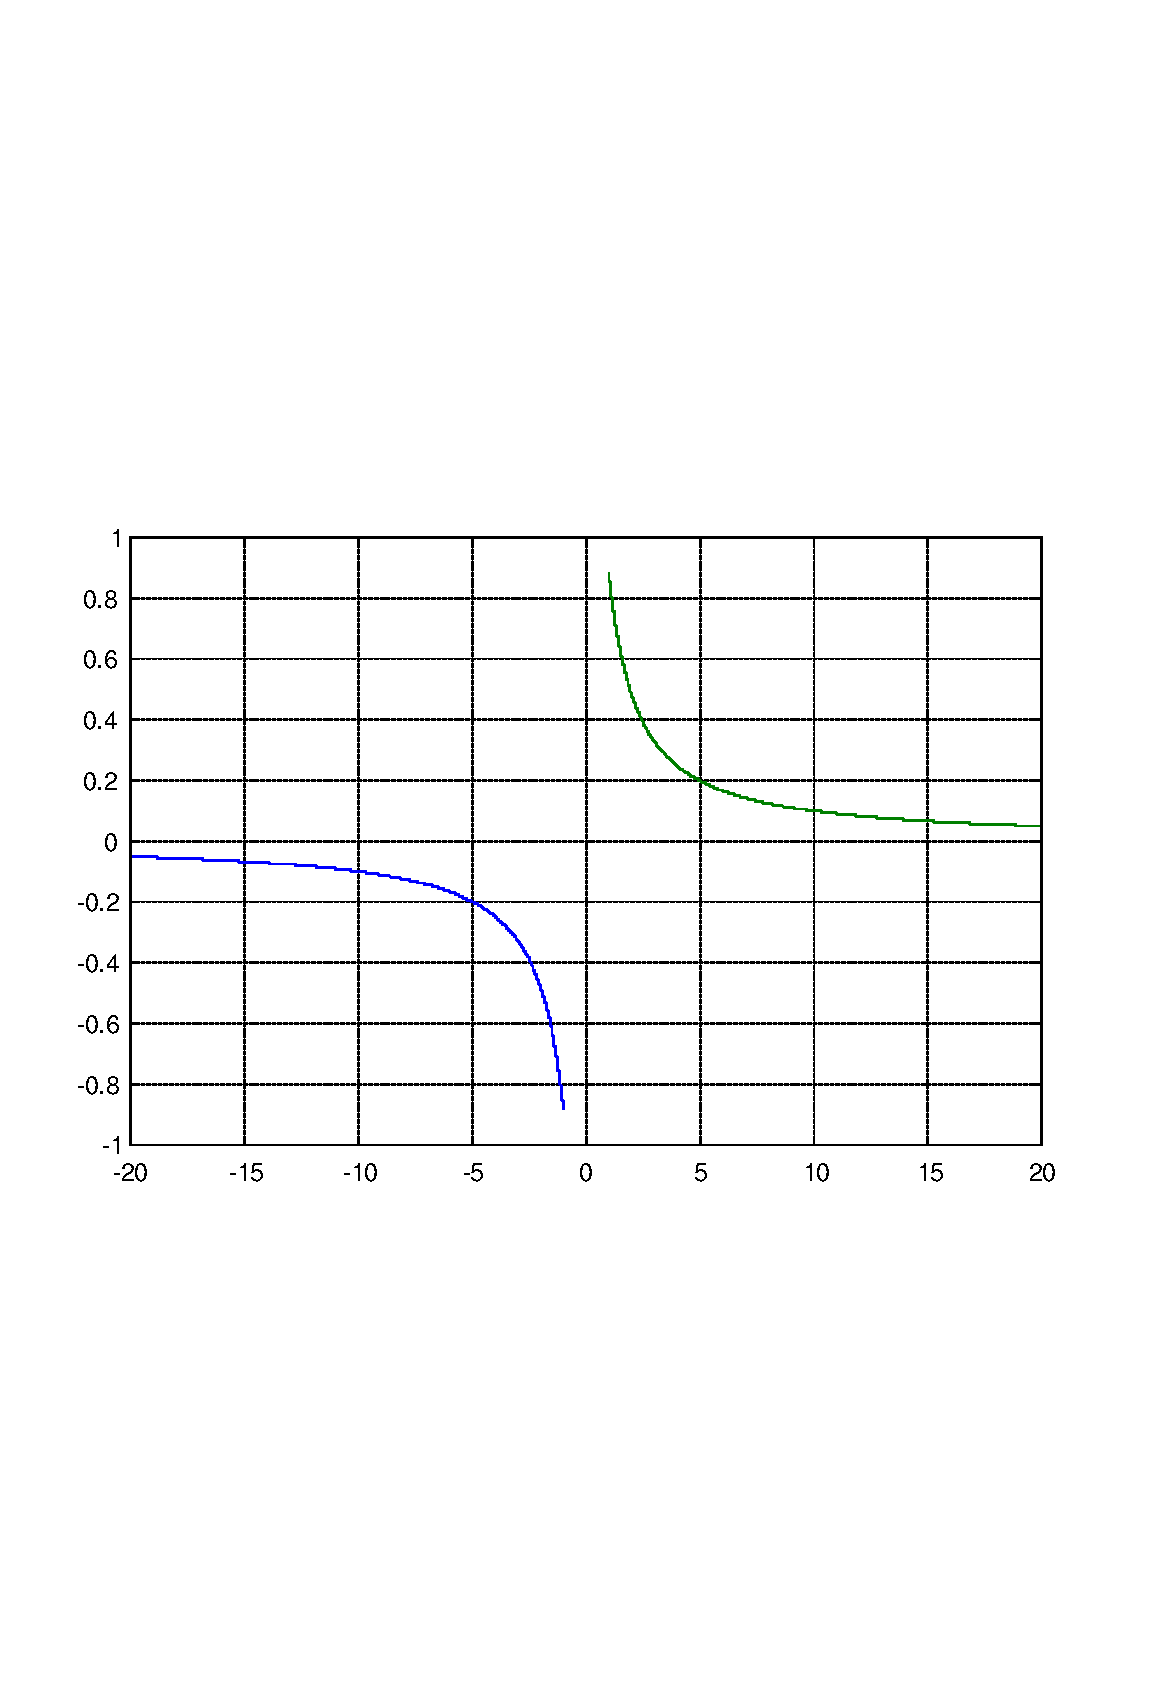
\includegraphics[width=12cm]{acschplot}
\caption{acschplot}
\end{DoxyImage}
 \hypertarget{mathfunctions_acscd}{}\section{A\-C\-S\-C\-D Inverse Cosecant Degrees Function}\label{mathfunctions_acscd}
Section\-: \hyperlink{sec_mathfunctions}{Mathematical Functions} \hypertarget{vtkwidgets_vtkxyplotwidget_Usage}{}\subsection{Usage}\label{vtkwidgets_vtkxyplotwidget_Usage}
Computes the inverse cosecant of the argument, but returns the argument in degrees instead of radians (as is the case for {\ttfamily acsc}. The syntax for its use is \begin{DoxyVerb}   y = acscd(x)
\end{DoxyVerb}
 \hypertarget{variables_matrix_Examples}{}\subsection{Examples}\label{variables_matrix_Examples}
The inverse cosecant of {\ttfamily 2/sqrt(2)} should be 45 degrees\-:


\begin{DoxyVerbInclude}
--> acscd(2/sqrt(2))

ans = 
   45.0000 
\end{DoxyVerbInclude}


and the inverse cosecant of {\ttfamily 2} should be 30 degrees\-:


\begin{DoxyVerbInclude}
--> acscd(0.5)

ans = 
  90.0000 - 75.4561i 
\end{DoxyVerbInclude}
 \hypertarget{mathfunctions_acsch}{}\section{A\-C\-S\-C\-H Inverse Hyperbolic Cosecant Function}\label{mathfunctions_acsch}
Section\-: \hyperlink{sec_mathfunctions}{Mathematical Functions} \hypertarget{vtkwidgets_vtkxyplotwidget_Usage}{}\subsection{Usage}\label{vtkwidgets_vtkxyplotwidget_Usage}
Computes the inverse hyperbolic cosecant of its argument. The general syntax for its use is \begin{DoxyVerb}  y = acsch(x)
\end{DoxyVerb}
 where {\ttfamily x} is an {\ttfamily n}-\/dimensional array of numerical type. \hypertarget{transforms_svd_Function}{}\subsection{Internals}\label{transforms_svd_Function}
The {\ttfamily acsch} function is computed from the formula \[ \mathrm{csch}^{-1}(x) = \sinh^{-1}\left(\frac{1}{x}\right) \] \hypertarget{variables_matrix_Examples}{}\subsection{Examples}\label{variables_matrix_Examples}
Here is a simple plot of the inverse hyperbolic cosecant function


\begin{DoxyVerbInclude}
--> x1 = -20:.01:-1;
--> x2 = 1:.01:20;
--> plot(x1,acsch(x1),x2,acsch(x2)); grid('on');
\end{DoxyVerbInclude}


 
\begin{DoxyImage}
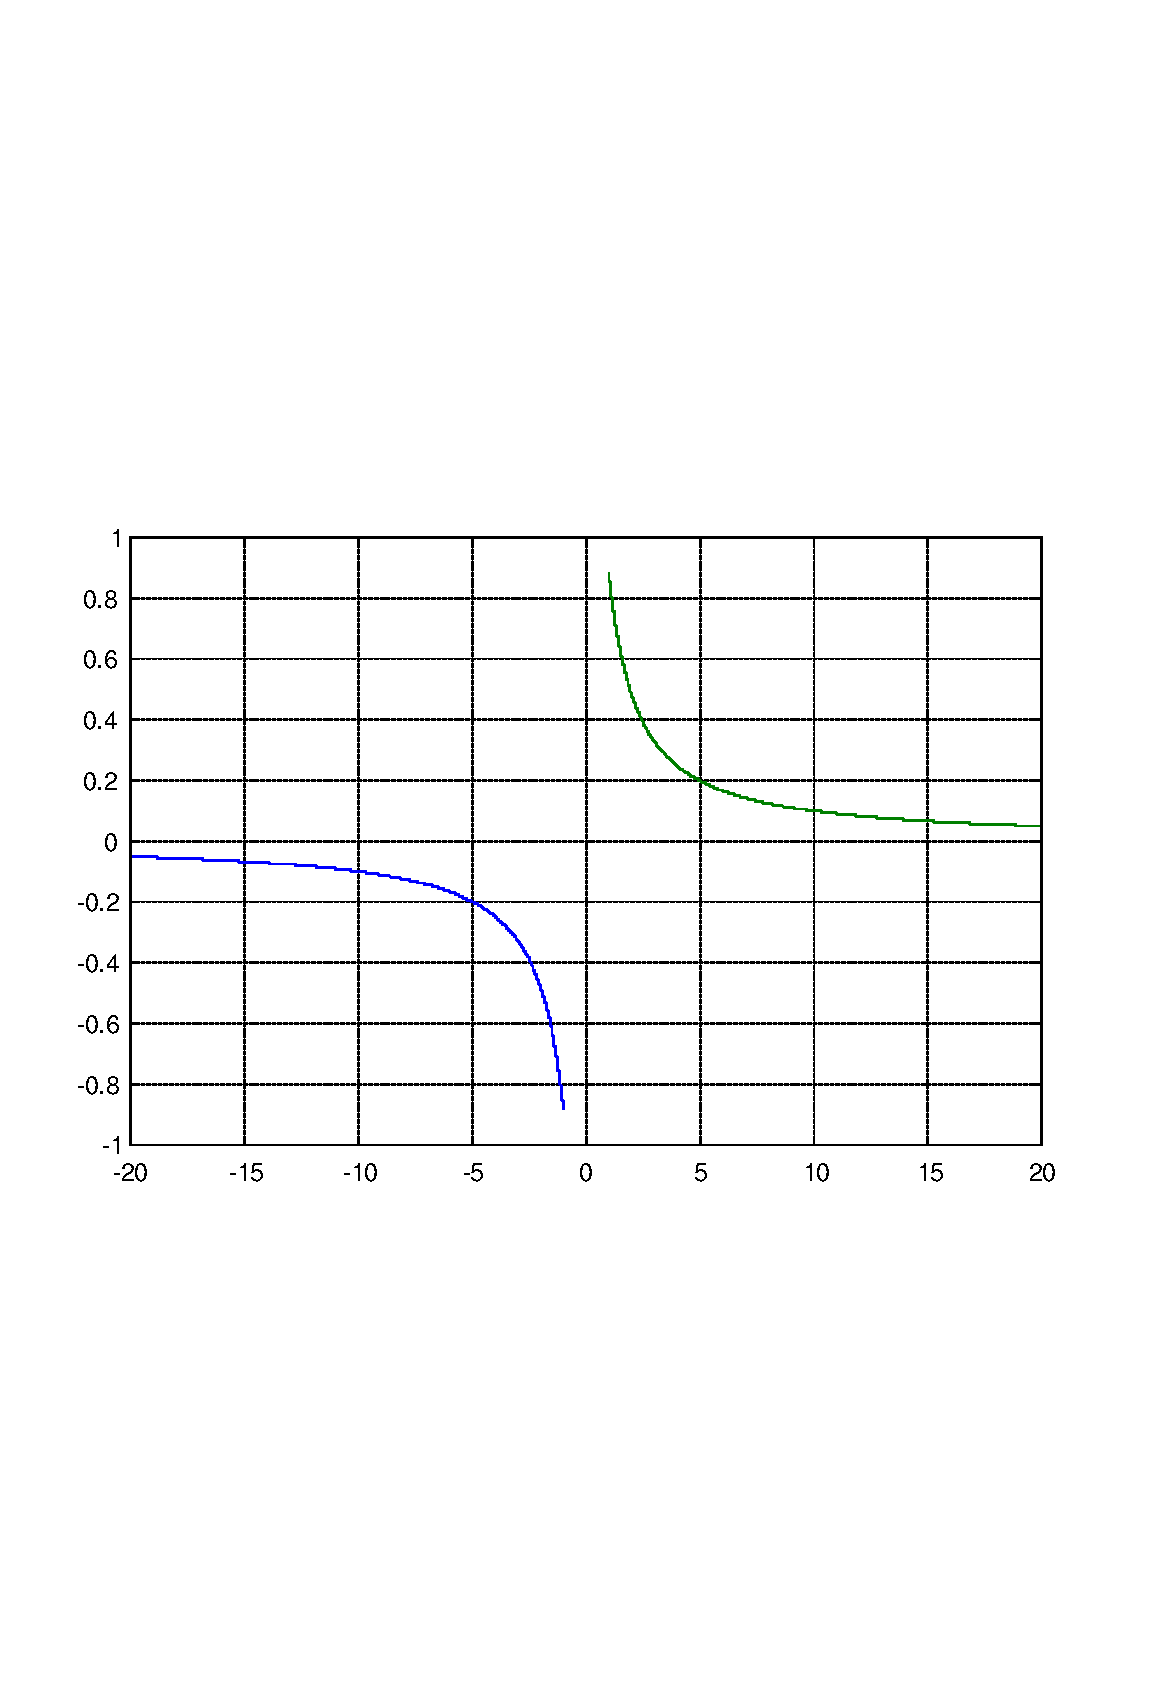
\includegraphics[width=12cm]{acschplot}
\caption{acschplot}
\end{DoxyImage}
 \hypertarget{mathfunctions_angle}{}\section{A\-N\-G\-L\-E Phase Angle Function}\label{mathfunctions_angle}
Section\-: \hyperlink{sec_mathfunctions}{Mathematical Functions} \hypertarget{vtkwidgets_vtkxyplotwidget_Usage}{}\subsection{Usage}\label{vtkwidgets_vtkxyplotwidget_Usage}
Compute the phase angle in radians of a complex matrix. The general syntax for its use is \begin{DoxyVerb}  p = angle(c)
\end{DoxyVerb}
 where {\ttfamily c} is an {\ttfamily n}-\/dimensional array of numerical type. \hypertarget{transforms_svd_Function}{}\subsection{Internals}\label{transforms_svd_Function}
For a complex number {\ttfamily x}, its polar representation is given by \[ x = |x| e^{j\theta} \] and we can compute \[ \theta = \mathrm{atan2}(\Im x, \Re x) \] \hypertarget{variables_struct_Example}{}\subsection{Example}\label{variables_struct_Example}
Here are some examples of the use of {\ttfamily angle} in the polar decomposition of a complex number.


\begin{DoxyVerbInclude}
--> x = 3+4*i

x = 
   3.0000 +  4.0000i 

--> a = abs(x)

a = 
 5 

--> t = angle(x)

t = 
    0.9273 

--> a*exp(i*t)

ans = 
   3.0000 +  4.0000i 
\end{DoxyVerbInclude}


M version contributor\-: M.\-W. Vogel 01-\/30-\/06 \hypertarget{mathfunctions_asec}{}\section{A\-S\-E\-C Inverse Secant Function}\label{mathfunctions_asec}
Section\-: \hyperlink{sec_mathfunctions}{Mathematical Functions} \hypertarget{vtkwidgets_vtkxyplotwidget_Usage}{}\subsection{Usage}\label{vtkwidgets_vtkxyplotwidget_Usage}
Computes the inverse secant of its argument. The general syntax for its use is \begin{DoxyVerb}  y = asec(x)
\end{DoxyVerb}
 where {\ttfamily x} is an {\ttfamily n}-\/dimensional array of numerical type. \hypertarget{transforms_svd_Function}{}\subsection{Internals}\label{transforms_svd_Function}
The {\ttfamily acosh} function is computed from the formula \[ \sec^{-1}(x) = \cos^{-1}\left(\frac{1}{x}\right) \] \hypertarget{variables_matrix_Examples}{}\subsection{Examples}\label{variables_matrix_Examples}
Here is a simple plot of the inverse secant function


\begin{DoxyVerbInclude}
--> x1 = -5:.01:-1;
--> x2 = 1:.01:5;
--> plot(x1,asec(x1),x2,asec(x2)); grid('on');
\end{DoxyVerbInclude}


 
\begin{DoxyImage}
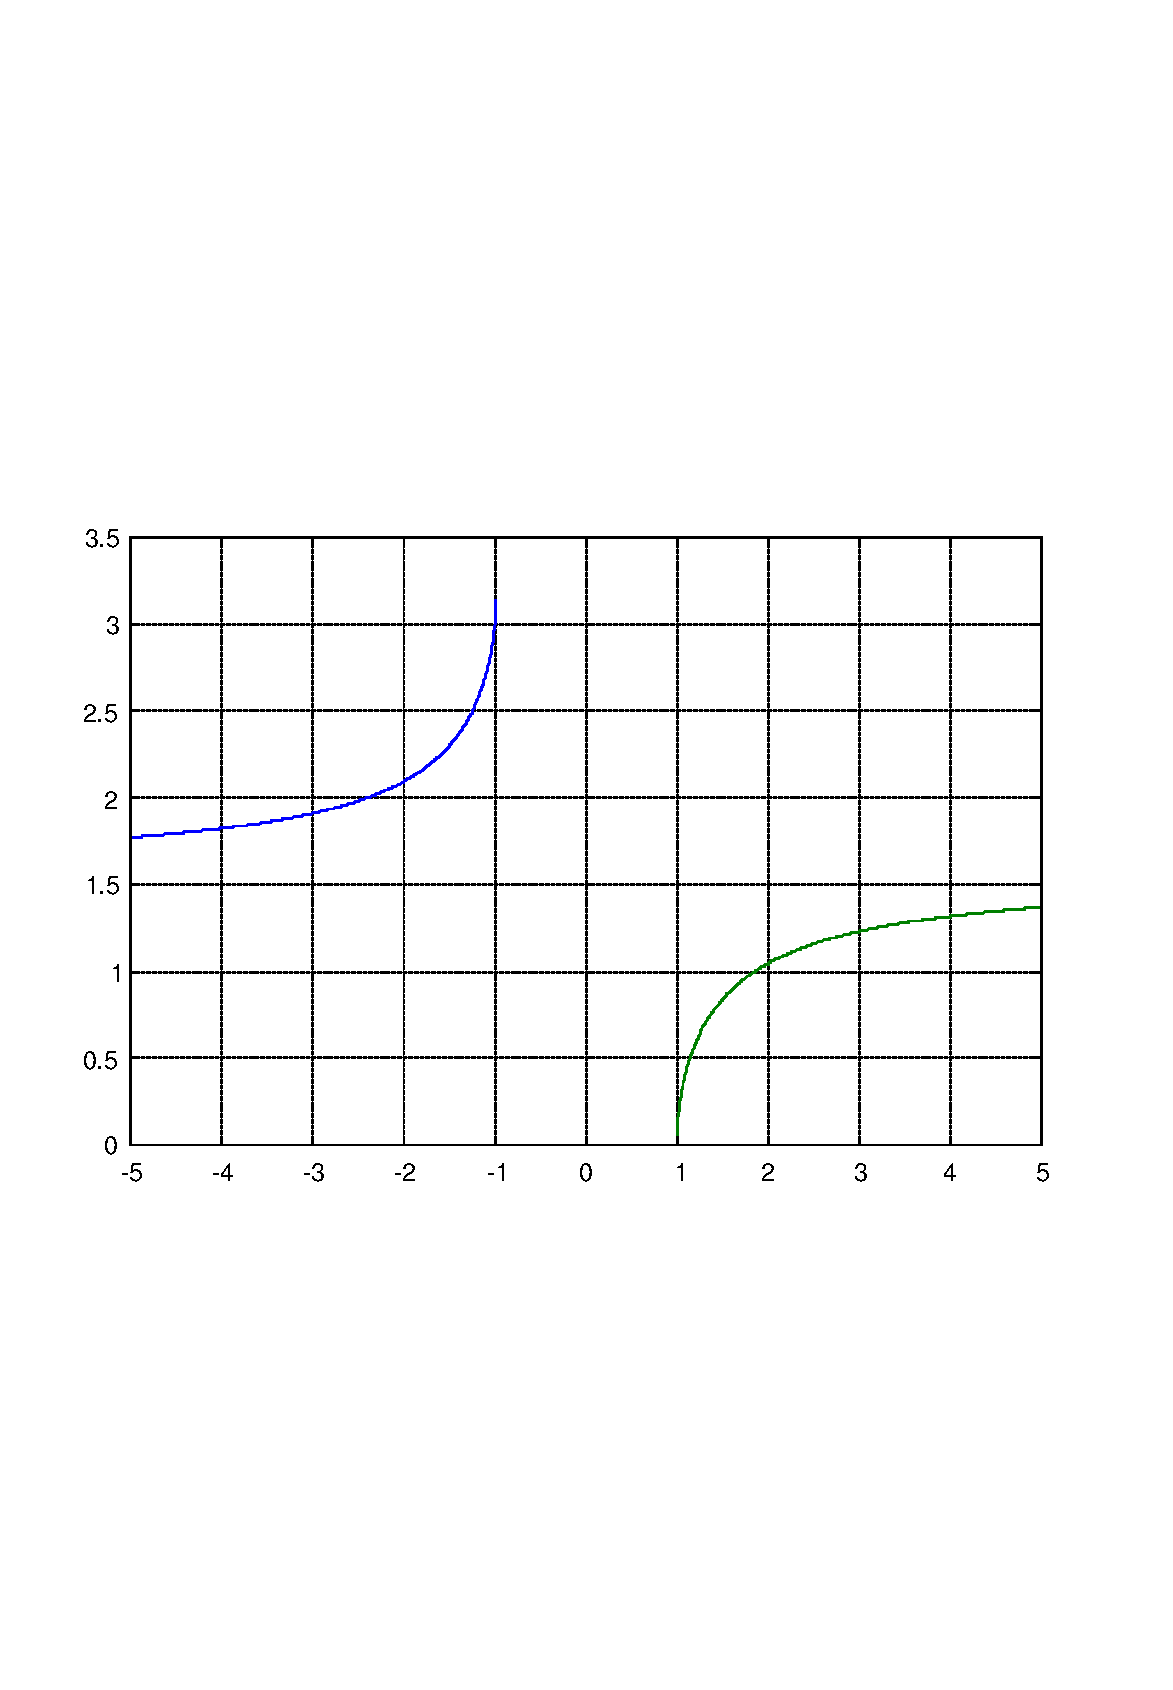
\includegraphics[width=12cm]{asecplot}
\caption{asecplot}
\end{DoxyImage}
 \hypertarget{mathfunctions_asecd}{}\section{A\-S\-E\-C\-D Inverse Secant Degrees Function}\label{mathfunctions_asecd}
Section\-: \hyperlink{sec_mathfunctions}{Mathematical Functions} \hypertarget{vtkwidgets_vtkxyplotwidget_Usage}{}\subsection{Usage}\label{vtkwidgets_vtkxyplotwidget_Usage}
Computes the inverse secant of the argument, but returns the argument in degrees instead of radians (as is the case for {\ttfamily asec}. The syntax for its use is \begin{DoxyVerb}   y = asecd(x)
\end{DoxyVerb}
 \hypertarget{variables_matrix_Examples}{}\subsection{Examples}\label{variables_matrix_Examples}
The inverse secant of {\ttfamily 2/sqrt(2)} should be 45 degrees\-:


\begin{DoxyVerbInclude}
--> asecd(2/sqrt(2))

ans = 
  45.0000 +  0.0000i 
\end{DoxyVerbInclude}


and the inverse secant of {\ttfamily 2} should be 60 degrees\-:


\begin{DoxyVerbInclude}
--> asecd(2)

ans = 
  60.0000 +  0.0000i 
\end{DoxyVerbInclude}
 \hypertarget{mathfunctions_asech}{}\section{A\-S\-E\-C\-H Inverse Hyperbolic Secant Function}\label{mathfunctions_asech}
Section\-: \hyperlink{sec_mathfunctions}{Mathematical Functions} \hypertarget{vtkwidgets_vtkxyplotwidget_Usage}{}\subsection{Usage}\label{vtkwidgets_vtkxyplotwidget_Usage}
Computes the inverse hyperbolic secant of its argument. The general syntax for its use is \begin{DoxyVerb}  y = asech(x)
\end{DoxyVerb}
 where {\ttfamily x} is an {\ttfamily n}-\/dimensional array of numerical type. \hypertarget{transforms_svd_Function}{}\subsection{Internals}\label{transforms_svd_Function}
The {\ttfamily asech} function is computed from the formula \[ \mathrm{sech}^{-1}(x) = \cosh^{-1}\left(\frac{1}{x}\right) \] \hypertarget{variables_matrix_Examples}{}\subsection{Examples}\label{variables_matrix_Examples}
Here is a simple plot of the inverse hyperbolic secant function


\begin{DoxyVerbInclude}
--> x1 = -20:.01:-1;
--> x2 = 1:.01:20;
--> plot(x1,imag(asech(x1)),x2,imag(asech(x2))); grid('on');
\end{DoxyVerbInclude}


 
\begin{DoxyImage}
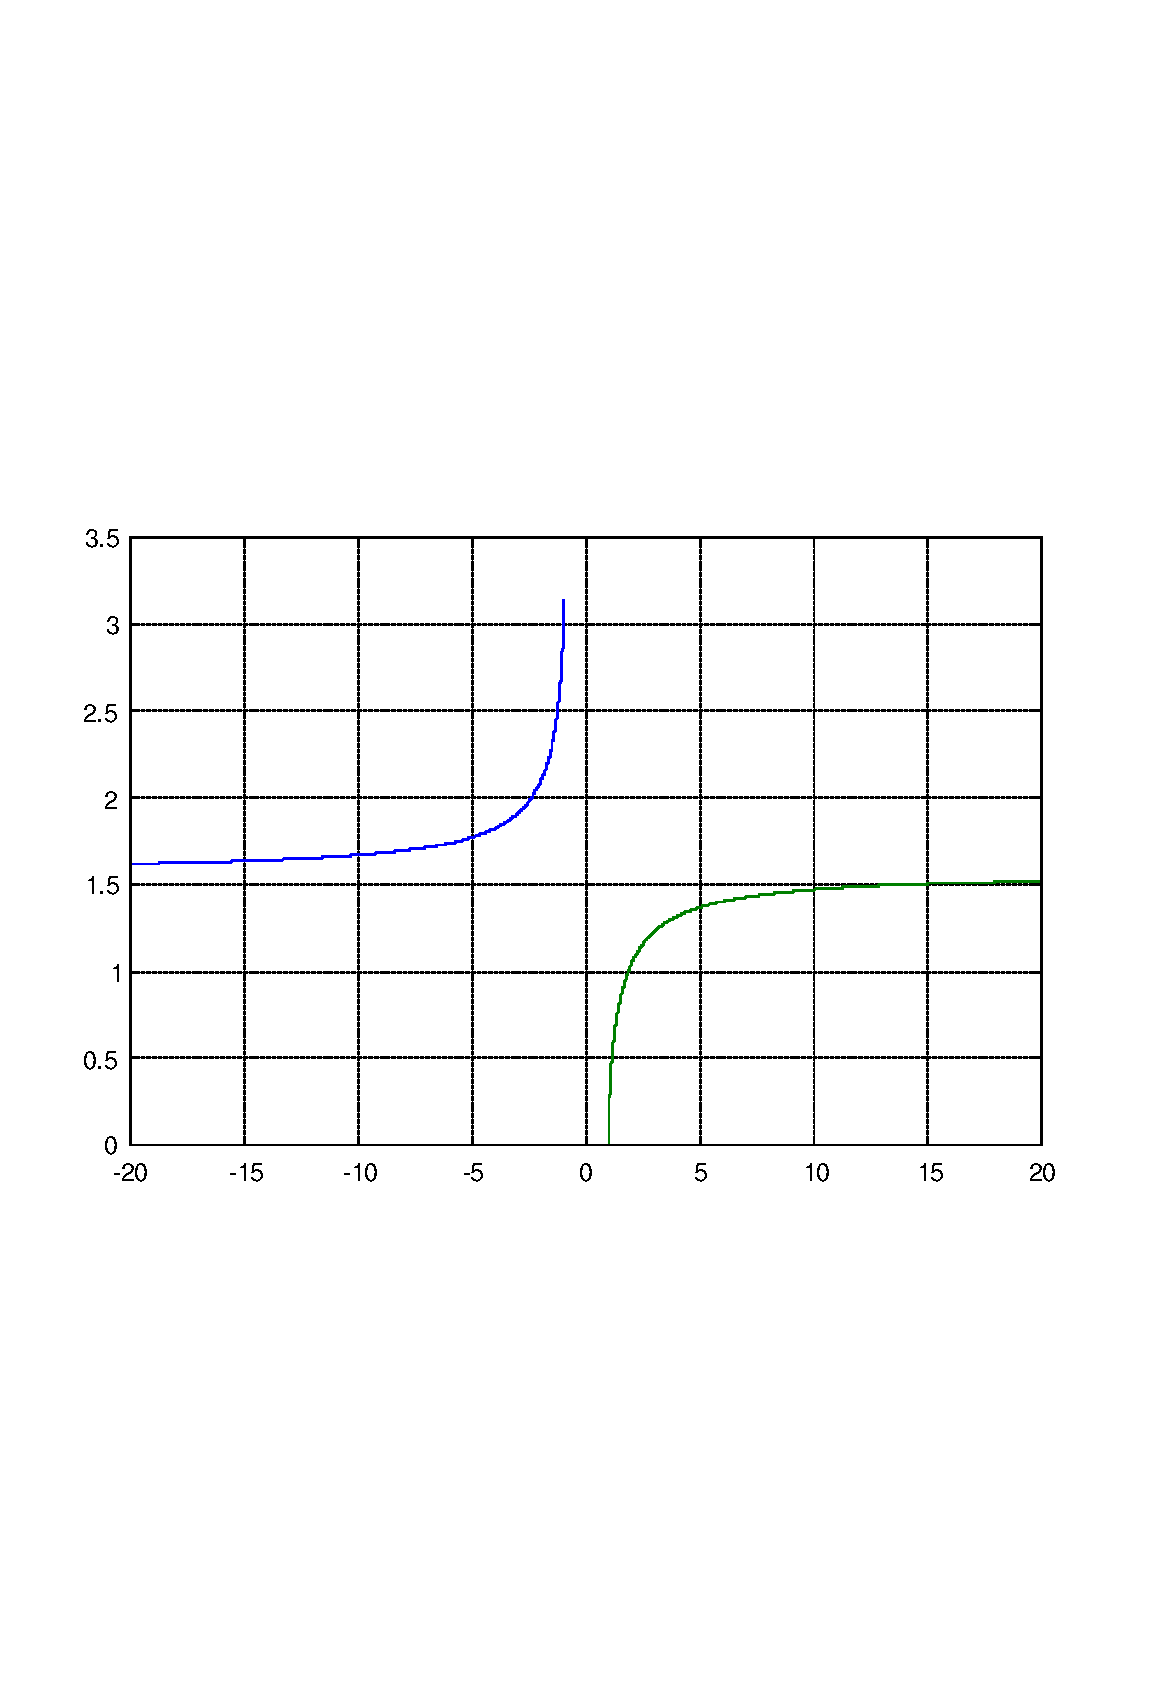
\includegraphics[width=12cm]{asechplot}
\caption{asechplot}
\end{DoxyImage}
 \hypertarget{mathfunctions_asin}{}\section{A\-S\-I\-N Inverse Trigonometric Arcsine Function}\label{mathfunctions_asin}
Section\-: \hyperlink{sec_mathfunctions}{Mathematical Functions} \hypertarget{vtkwidgets_vtkxyplotwidget_Usage}{}\subsection{Usage}\label{vtkwidgets_vtkxyplotwidget_Usage}
Computes the {\ttfamily asin} function for its argument. The general syntax for its use is \begin{DoxyVerb}  y = asin(x)
\end{DoxyVerb}
 where {\ttfamily x} is an {\ttfamily n}-\/dimensional array of numerical type. Integer types are promoted to the {\ttfamily double} type prior to calculation of the {\ttfamily asin} function. Output {\ttfamily y} is of the same size and type as the input {\ttfamily x}, (unless {\ttfamily x} is an integer, in which case {\ttfamily y} is a {\ttfamily double} type). \hypertarget{transforms_svd_Function}{}\subsection{Internals}\label{transforms_svd_Function}
Mathematically, the {\ttfamily asin} function is defined for all arguments {\ttfamily x} as \[ \mathrm{asin} x \equiv - i \log \left(i x + \sqrt{1-x^2}\right). \] For real valued variables {\ttfamily x} in the range {\ttfamily \mbox{[}-\/1,1\mbox{]}}, the function is computed directly using the standard C library's numerical {\ttfamily asin} function. For both real and complex arguments {\ttfamily x}, note that generally \[ \mathrm{asin}(\sin(x)) \neq x, \] due to the periodicity of {\ttfamily sin(x)}. \hypertarget{variables_struct_Example}{}\subsection{Example}\label{variables_struct_Example}
The following code demonstates the {\ttfamily asin} function over the range {\ttfamily \mbox{[}-\/1,1\mbox{]}}.


\begin{DoxyVerbInclude}
--> t = linspace(-1,1);
--> plot(t,asin(t))
\end{DoxyVerbInclude}


 
\begin{DoxyImage}
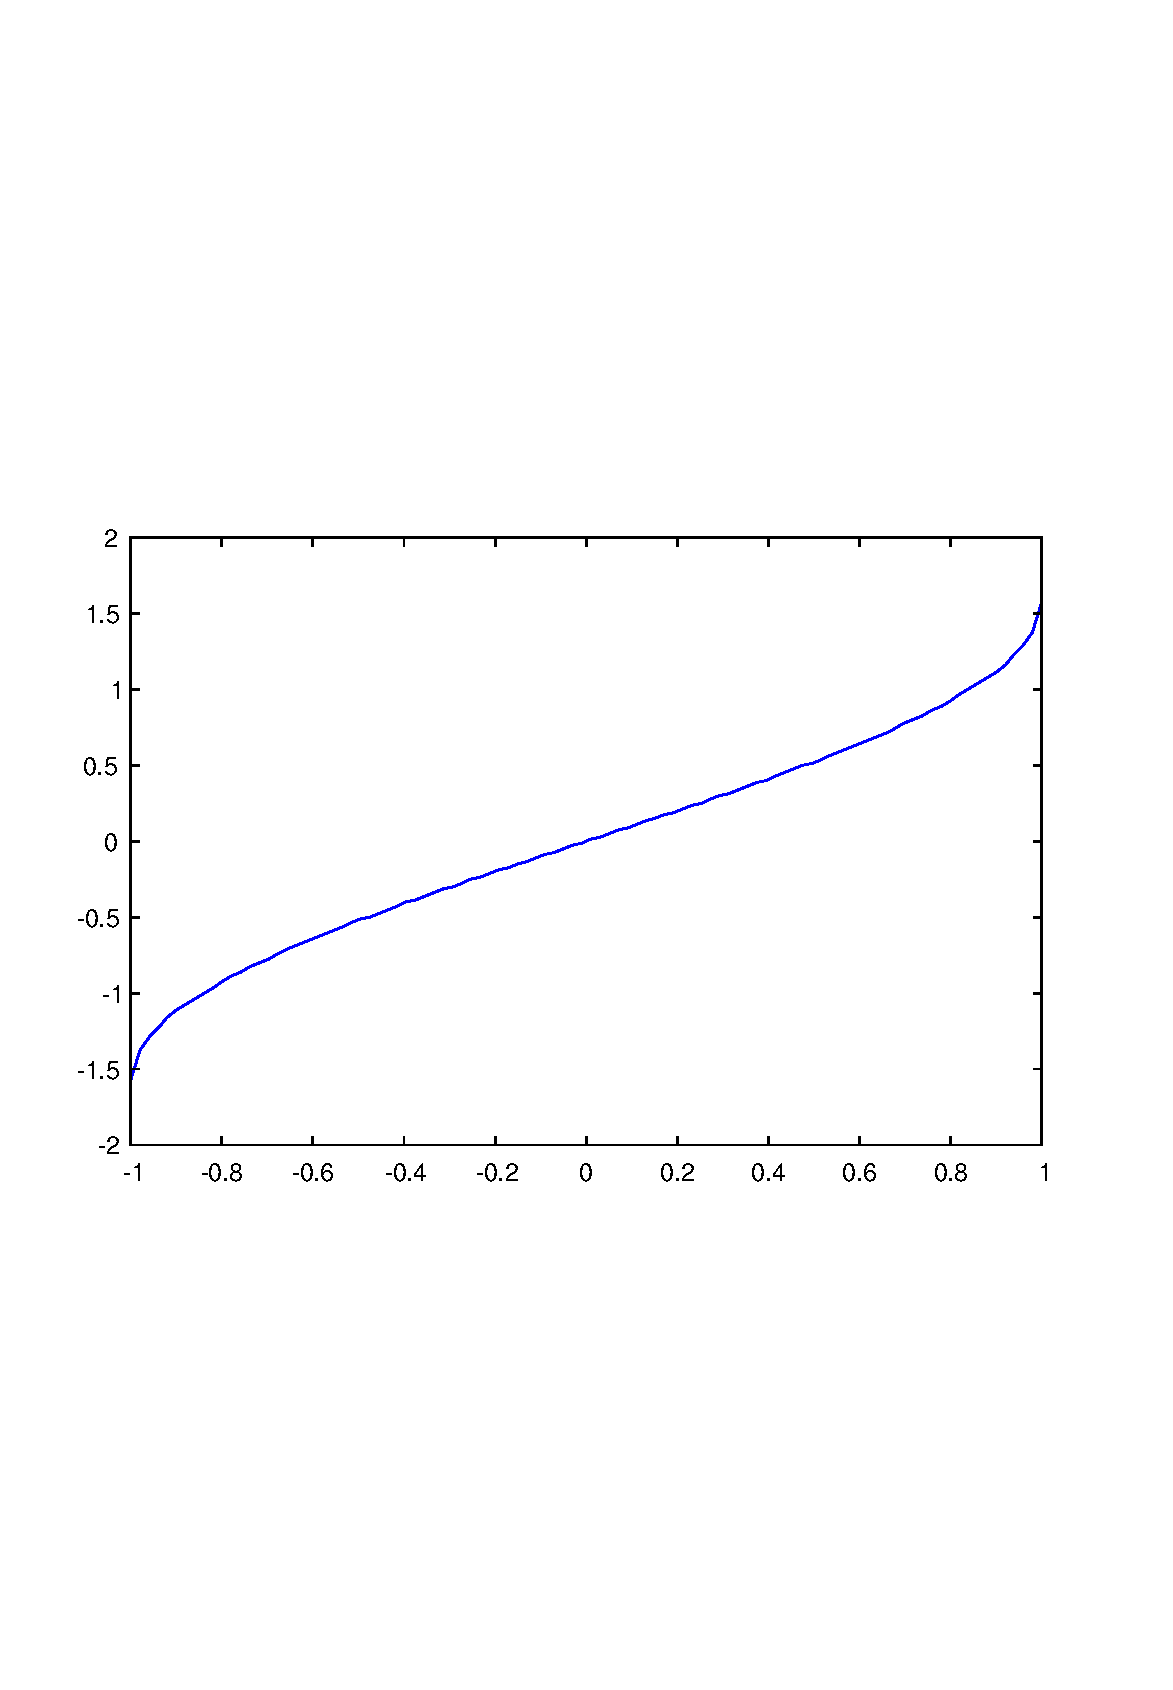
\includegraphics[width=12cm]{asinplot}
\caption{asinplot}
\end{DoxyImage}
 \hypertarget{mathfunctions_asind}{}\section{A\-S\-I\-N\-D Inverse Sine Degrees Function}\label{mathfunctions_asind}
Section\-: \hyperlink{sec_mathfunctions}{Mathematical Functions} \hypertarget{vtkwidgets_vtkxyplotwidget_Usage}{}\subsection{Usage}\label{vtkwidgets_vtkxyplotwidget_Usage}
Computes the inverse sine of the argument, but returns the argument in degrees instead of radians (as is the case for {\ttfamily asin}). The syntax for its use is \begin{DoxyVerb}   y = asind(x)
\end{DoxyVerb}
 \hypertarget{variables_matrix_Examples}{}\subsection{Examples}\label{variables_matrix_Examples}
The inverse sine of {\ttfamily sqrt(2)/2} should be 45 degrees\-:


\begin{DoxyVerbInclude}
--> asind(sqrt(2)/2)

ans = 
   45.0000 
\end{DoxyVerbInclude}


and the inverse sine of {\ttfamily 0.\-5} should be 30 degrees\-:


\begin{DoxyVerbInclude}
--> asind(0.5)

ans = 
   30.0000 
\end{DoxyVerbInclude}
 \hypertarget{mathfunctions_asinh}{}\section{A\-S\-I\-N\-H Inverse Hyperbolic Sine Function}\label{mathfunctions_asinh}
Section\-: \hyperlink{sec_mathfunctions}{Mathematical Functions} \hypertarget{vtkwidgets_vtkxyplotwidget_Usage}{}\subsection{Usage}\label{vtkwidgets_vtkxyplotwidget_Usage}
Computes the inverse hyperbolic sine of its argument. The general syntax for its use is \begin{DoxyVerb}  y = asinh(x)
\end{DoxyVerb}
 where {\ttfamily x} is an {\ttfamily n}-\/dimensional array of numerical type. \hypertarget{transforms_svd_Function}{}\subsection{Internals}\label{transforms_svd_Function}
The {\ttfamily asinh} function is computed from the formula \[ \sinh^{-1}(x) = \log\left(x + (x^2 + 1)^0.5\right) \] where the {\ttfamily log} (and square root) is taken in its most general sense. \hypertarget{variables_matrix_Examples}{}\subsection{Examples}\label{variables_matrix_Examples}
Here is a simple plot of the inverse hyperbolic sine function


\begin{DoxyVerbInclude}
--> x = -5:.01:5;
--> plot(x,asinh(x)); grid('on');
\end{DoxyVerbInclude}


 
\begin{DoxyImage}
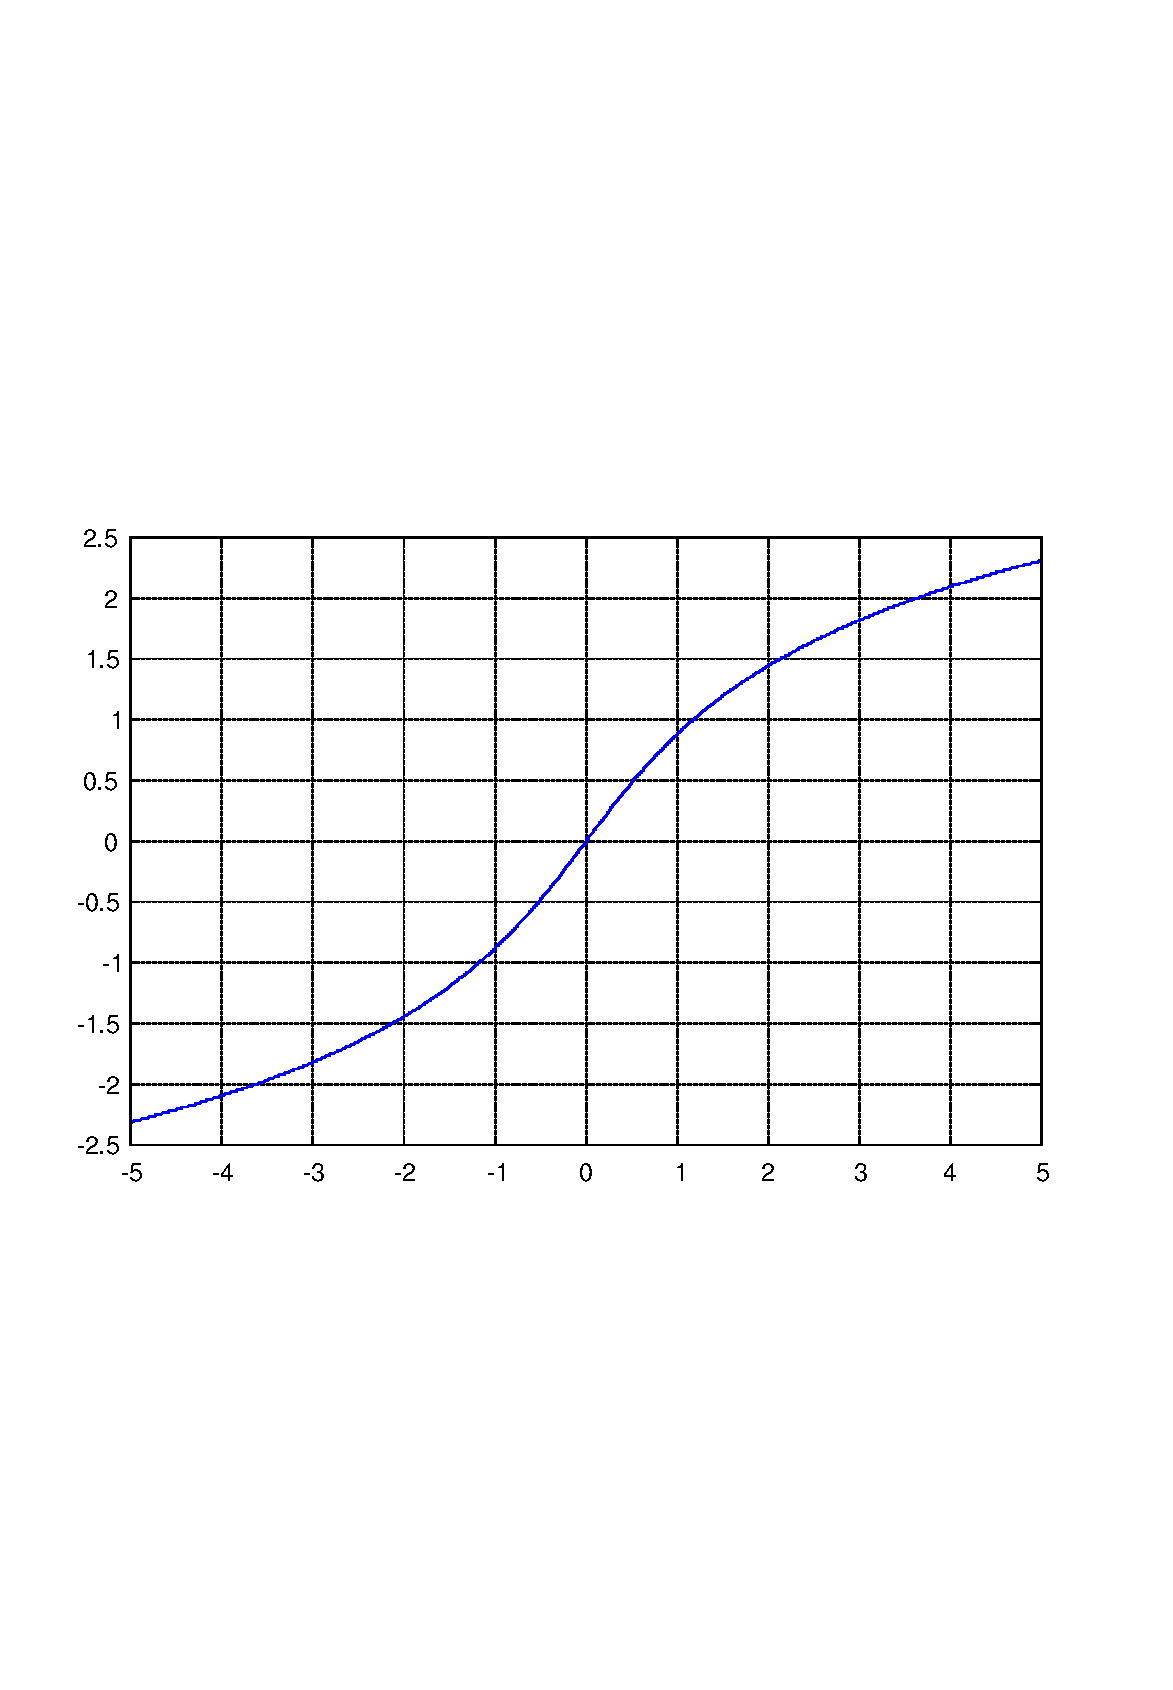
\includegraphics[width=12cm]{asinhplot}
\caption{asinhplot}
\end{DoxyImage}
 \hypertarget{mathfunctions_atan}{}\section{A\-T\-A\-N Inverse Trigonometric Arctangent Function}\label{mathfunctions_atan}
Section\-: \hyperlink{sec_mathfunctions}{Mathematical Functions} \hypertarget{vtkwidgets_vtkxyplotwidget_Usage}{}\subsection{Usage}\label{vtkwidgets_vtkxyplotwidget_Usage}
Computes the {\ttfamily atan} function for its argument. The general syntax for its use is \begin{DoxyVerb}  y = atan(x)
\end{DoxyVerb}
 where {\ttfamily x} is an {\ttfamily n}-\/dimensional array of numerical type. Integer types are promoted to the {\ttfamily double} type prior to calculation of the {\ttfamily atan} function. Output {\ttfamily y} is of the same size and type as the input {\ttfamily x}, (unless {\ttfamily x} is an integer, in which case {\ttfamily y} is a {\ttfamily double} type). \hypertarget{transforms_svd_Function}{}\subsection{Internals}\label{transforms_svd_Function}
Mathematically, the {\ttfamily atan} function is defined for all arguments {\ttfamily x} as \[ \mathrm{atan} x \equiv \frac{i}{2}\left(\log(1-i x) - \log(i x + 1)\right). \] For real valued variables {\ttfamily x}, the function is computed directly using the standard C library's numerical {\ttfamily atan} function. For both real and complex arguments {\ttfamily x}, note that generally

\[ \mathrm{atan}(\tan(x)) \neq x, \] due to the periodicity of {\ttfamily tan(x)}. \hypertarget{variables_struct_Example}{}\subsection{Example}\label{variables_struct_Example}
The following code demonstates the {\ttfamily atan} function over the range {\ttfamily \mbox{[}-\/1,1\mbox{]}}.


\begin{DoxyVerbInclude}
--> t = linspace(-1,1);
--> plot(t,atan(t))
\end{DoxyVerbInclude}


 
\begin{DoxyImage}
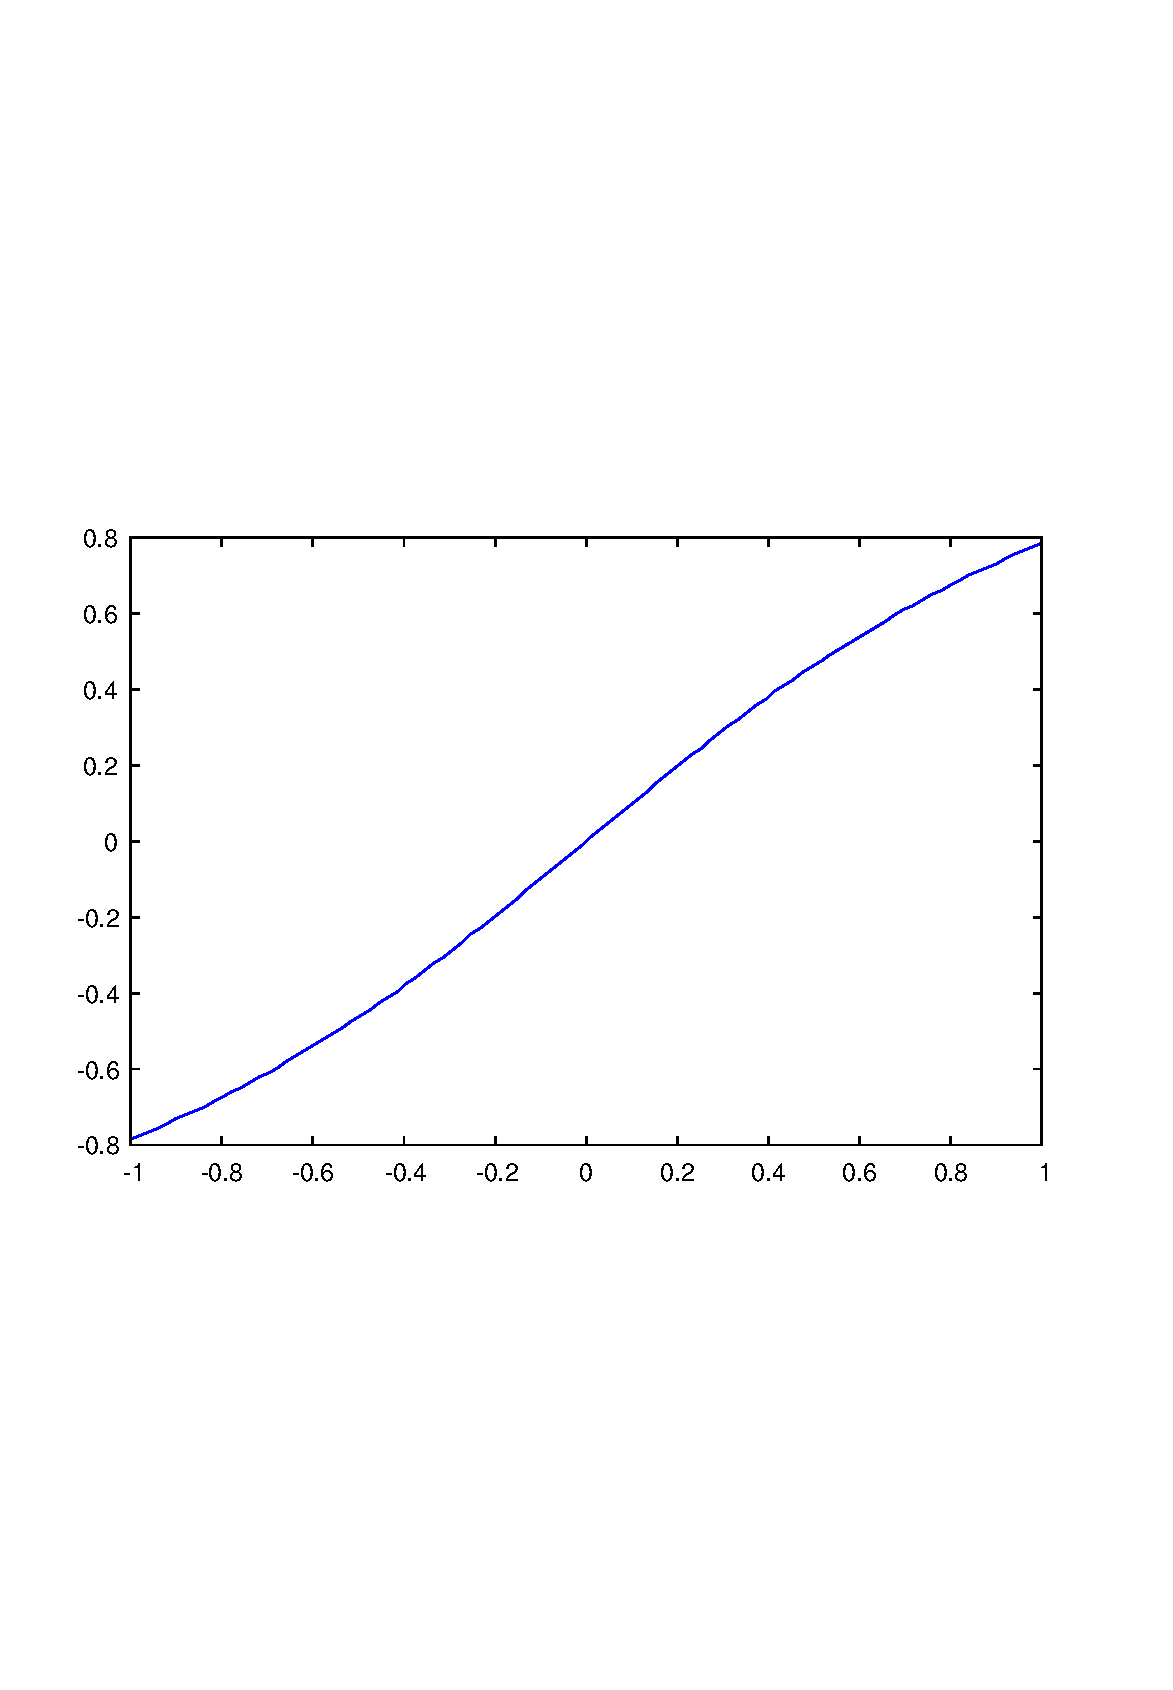
\includegraphics[width=12cm]{atanplot}
\caption{atanplot}
\end{DoxyImage}
 \hypertarget{mathfunctions_atan2}{}\section{A\-T\-A\-N2 Inverse Trigonometric 4-\/\-Quadrant Arctangent Function}\label{mathfunctions_atan2}
Section\-: \hyperlink{sec_mathfunctions}{Mathematical Functions} \hypertarget{vtkwidgets_vtkxyplotwidget_Usage}{}\subsection{Usage}\label{vtkwidgets_vtkxyplotwidget_Usage}
Computes the {\ttfamily atan2} function for its argument. The general syntax for its use is \begin{DoxyVerb}  z = atan2(y,x)
\end{DoxyVerb}
 where {\ttfamily x} and {\ttfamily y} are {\ttfamily n}-\/dimensional arrays of numerical type. Integer types are promoted to the {\ttfamily double} type prior to calculation of the {\ttfamily atan2} function. The size of the output depends on the size of {\ttfamily x} and {\ttfamily y}. If {\ttfamily x} is a scalar, then {\ttfamily z} is the same size as {\ttfamily y}, and if {\ttfamily y} is a scalar, then {\ttfamily z} is the same size as {\ttfamily x}. The type of the output is equal to the type of $|$y/x$|$. \hypertarget{transforms_svd_Function}{}\subsection{Internals}\label{transforms_svd_Function}
The function is defined (for real values) to return an angle between {\ttfamily -\/pi} and {\ttfamily pi}. The signs of {\ttfamily x} and {\ttfamily y} are used to find the correct quadrant for the solution. For complex arguments, the two-\/argument arctangent is computed via \[ \mathrm{atan2}(y,x) \equiv -i \log\left(\frac{x+i y}{\sqrt{x^2+y^2}} \right) \] For real valued arguments {\ttfamily x,y}, the function is computed directly using the standard C library's numerical {\ttfamily atan2} function. For both real and complex arguments {\ttfamily x}, note that generally \[ \mathrm{atan2}(\sin(x),\cos(x)) \neq x, \] due to the periodicities of {\ttfamily cos(x)} and {\ttfamily sin(x)}. \hypertarget{variables_struct_Example}{}\subsection{Example}\label{variables_struct_Example}
The following code demonstates the difference between the {\ttfamily atan2} function and the {\ttfamily atan} function over the range {\ttfamily \mbox{[}-\/pi,pi\mbox{]}}.


\begin{DoxyVerbInclude}
--> x = linspace(-pi,pi);
--> sx = sin(x); cx = cos(x);
--> plot(x,atan(sx./cx),x,atan2(sx,cx))
\end{DoxyVerbInclude}


 
\begin{DoxyImage}
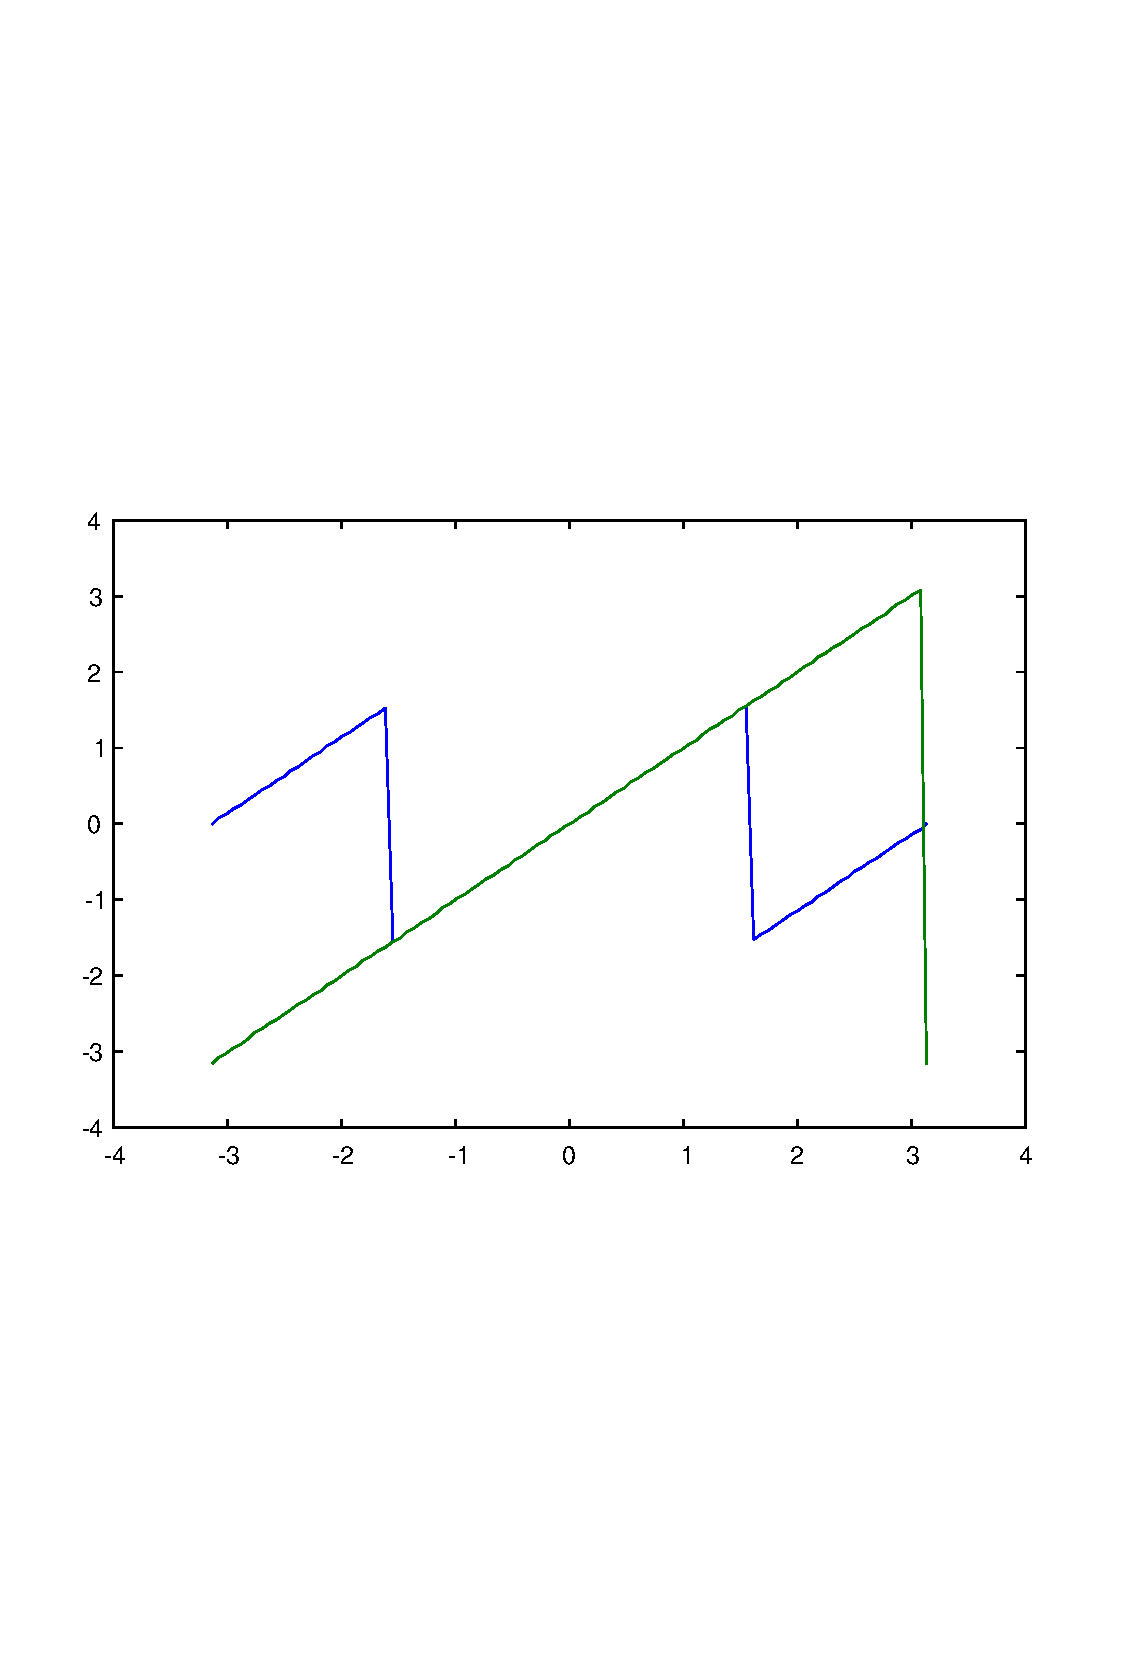
\includegraphics[width=12cm]{atan2plot}
\caption{atan2plot}
\end{DoxyImage}
 Note how the two-\/argument {\ttfamily atan2} function (green line) correctly ``unwraps'' the phase of the angle, while the {\ttfamily atan} function (red line) wraps the angle to the interval $[-\pi/2,\pi/2]$. \hypertarget{mathfunctions_atand}{}\section{A\-T\-A\-N\-D Inverse Tangent Degrees Function}\label{mathfunctions_atand}
Section\-: \hyperlink{sec_mathfunctions}{Mathematical Functions} \hypertarget{vtkwidgets_vtkxyplotwidget_Usage}{}\subsection{Usage}\label{vtkwidgets_vtkxyplotwidget_Usage}
Computes the inverse tangent of the argument, but returns the argument in degrees instead of radians (as is the case for {\ttfamily atan}. The syntax for its use is \begin{DoxyVerb}   y = atand(x)
\end{DoxyVerb}
 \hypertarget{variables_matrix_Examples}{}\subsection{Examples}\label{variables_matrix_Examples}
The inverse tangent of {\ttfamily 1} should be 45 degrees\-:


\begin{DoxyVerbInclude}
--> atand(1)

ans = 
 45 
\end{DoxyVerbInclude}
 \hypertarget{mathfunctions_atanh}{}\section{A\-T\-A\-N\-H Inverse Hyperbolic Tangent Function}\label{mathfunctions_atanh}
Section\-: \hyperlink{sec_mathfunctions}{Mathematical Functions} \hypertarget{vtkwidgets_vtkxyplotwidget_Usage}{}\subsection{Usage}\label{vtkwidgets_vtkxyplotwidget_Usage}
Computes the inverse hyperbolic tangent of its argument. The general syntax for its use is \begin{DoxyVerb}  y = atanh(x)
\end{DoxyVerb}
 where {\ttfamily x} is an {\ttfamily n}-\/dimensional array of numerical type. \hypertarget{transforms_svd_Function}{}\subsection{Internals}\label{transforms_svd_Function}
The {\ttfamily atanh} function is computed from the formula \[ \tanh^{-1}(x) = \frac{1}{2}\log\left(\frac{1+x}{1-x}\right) \] where the {\ttfamily log} (and square root) is taken in its most general sense. \hypertarget{variables_matrix_Examples}{}\subsection{Examples}\label{variables_matrix_Examples}
Here is a simple plot of the inverse hyperbolic tangent function


\begin{DoxyVerbInclude}
--> x = -0.99:.01:0.99;
--> plot(x,atanh(x)); grid('on');
\end{DoxyVerbInclude}


 
\begin{DoxyImage}
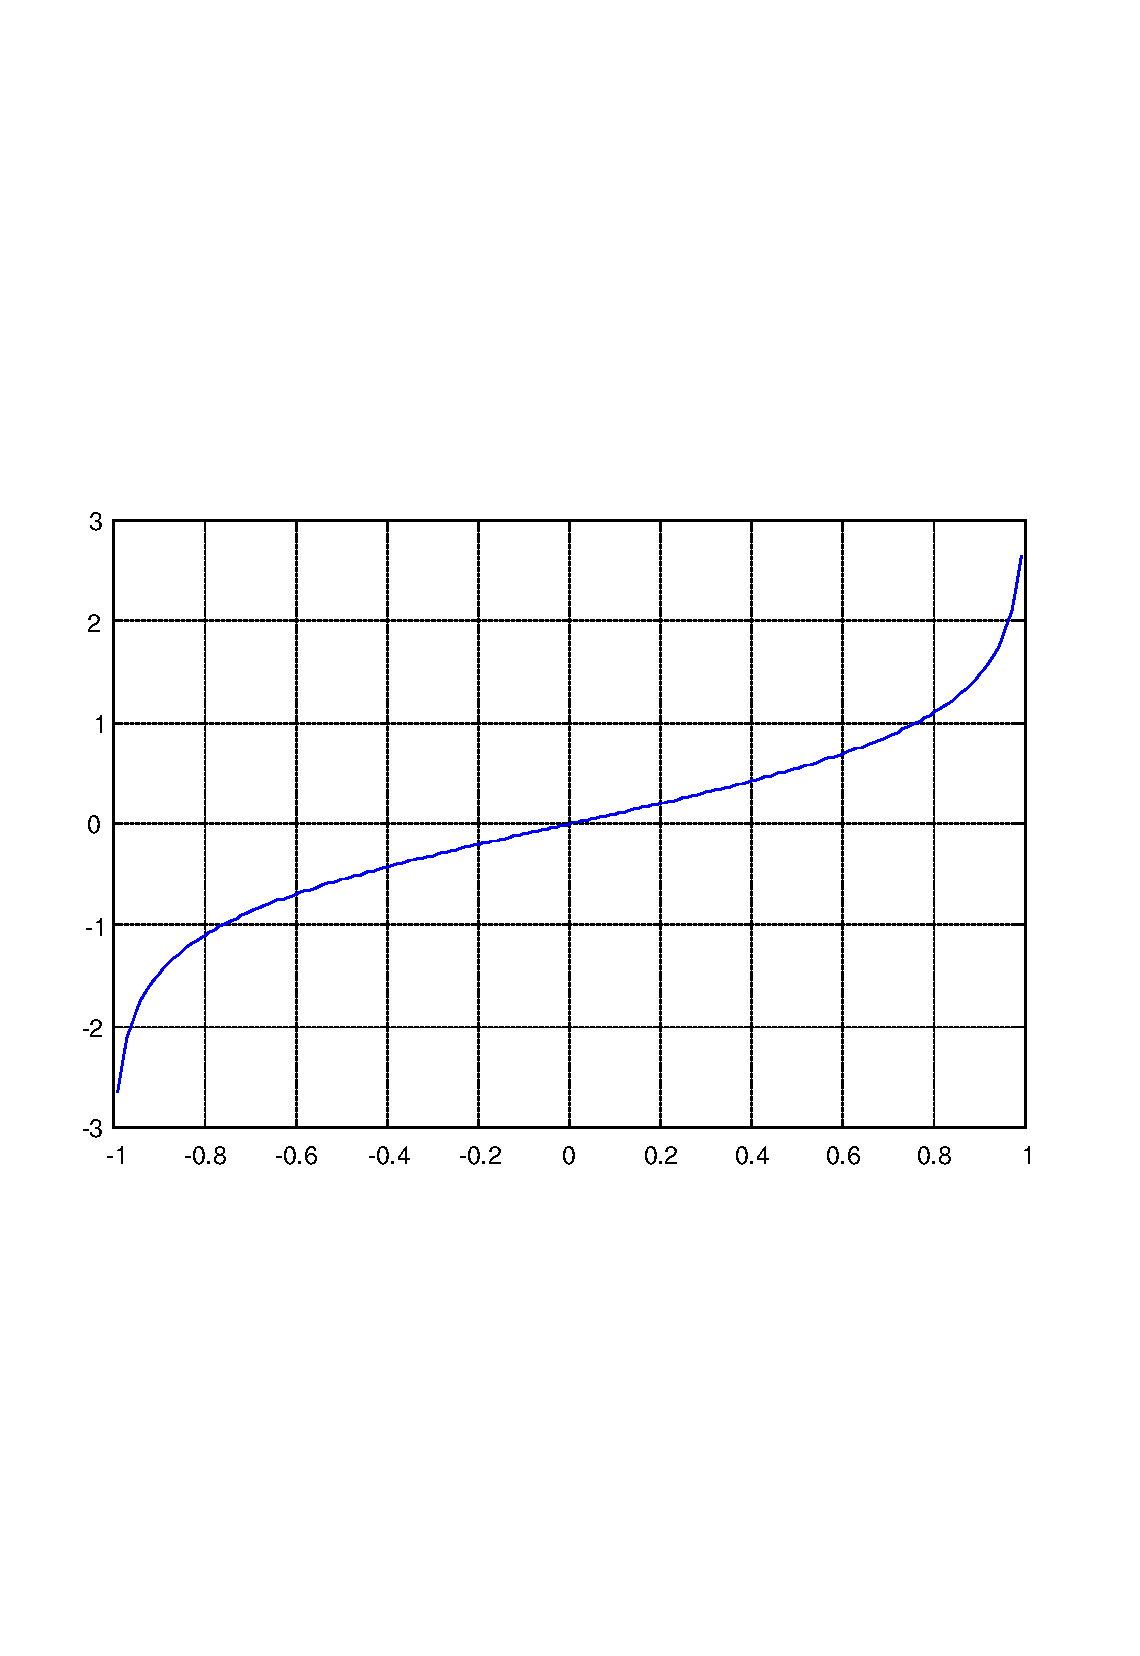
\includegraphics[width=12cm]{atanhplot}
\caption{atanhplot}
\end{DoxyImage}
 \hypertarget{mathfunctions_betainc}{}\section{B\-E\-T\-A\-I\-N\-C Incomplete Beta Function}\label{mathfunctions_betainc}
Section\-: \hyperlink{sec_mathfunctions}{Mathematical Functions} \hypertarget{vtkwidgets_vtkxyplotwidget_Usage}{}\subsection{Usage}\label{vtkwidgets_vtkxyplotwidget_Usage}
Computes the incomplete beta function. The {\ttfamily betainc} function takes 3 or 4 arguments \begin{DoxyVerb}  A = betainc(X,Y,Z)
\end{DoxyVerb}
 \begin{DoxyVerb}  A = betainc(X,Y,Z,tail)
\end{DoxyVerb}
 where {\ttfamily X} is either a {\ttfamily float} or {\ttfamily double} array with elements in \mbox{[}0,1\mbox{]} interval, {\ttfamily Y} and {\ttfamily Z} are real non-\/negative arrays. {\ttfamily tail} specifies the tail of the incomplete beta function. If {\ttfamily tail} is 'lower' (default) than the integral from 0 to x is computed. If {\ttfamily tail} is 'upper' than the integral from x to 1 is computed. All arrays must be the same size or be scalar. The output vector {\ttfamily A} is the same size (and type) as input arrays. \hypertarget{transforms_svd_Function}{}\subsection{Internals}\label{transforms_svd_Function}
The incomplete beta function is defined by the integral\-: \[ BetaI_x(a,b)=B_x(a,b)/B(a,b) where B_x(a,b) = \int_0^x t^{a-1} (1-t)^{b-1} dt for 0 <= x <= 1. For a > 0, b > 0 \] \hypertarget{variables_struct_Example}{}\subsection{Example}\label{variables_struct_Example}
Here is a plot of the betainc function over the range {\ttfamily \mbox{[}.2,.8\mbox{]}}.


\begin{DoxyVerbInclude}
--> x=.2:.01:.8;
--> y = betainc(x,5,3);
--> plot(x,y); xlabel('x'); ylabel('betainc(x,5,3)');
\end{DoxyVerbInclude}


which results in the following plot.  
\begin{DoxyImage}
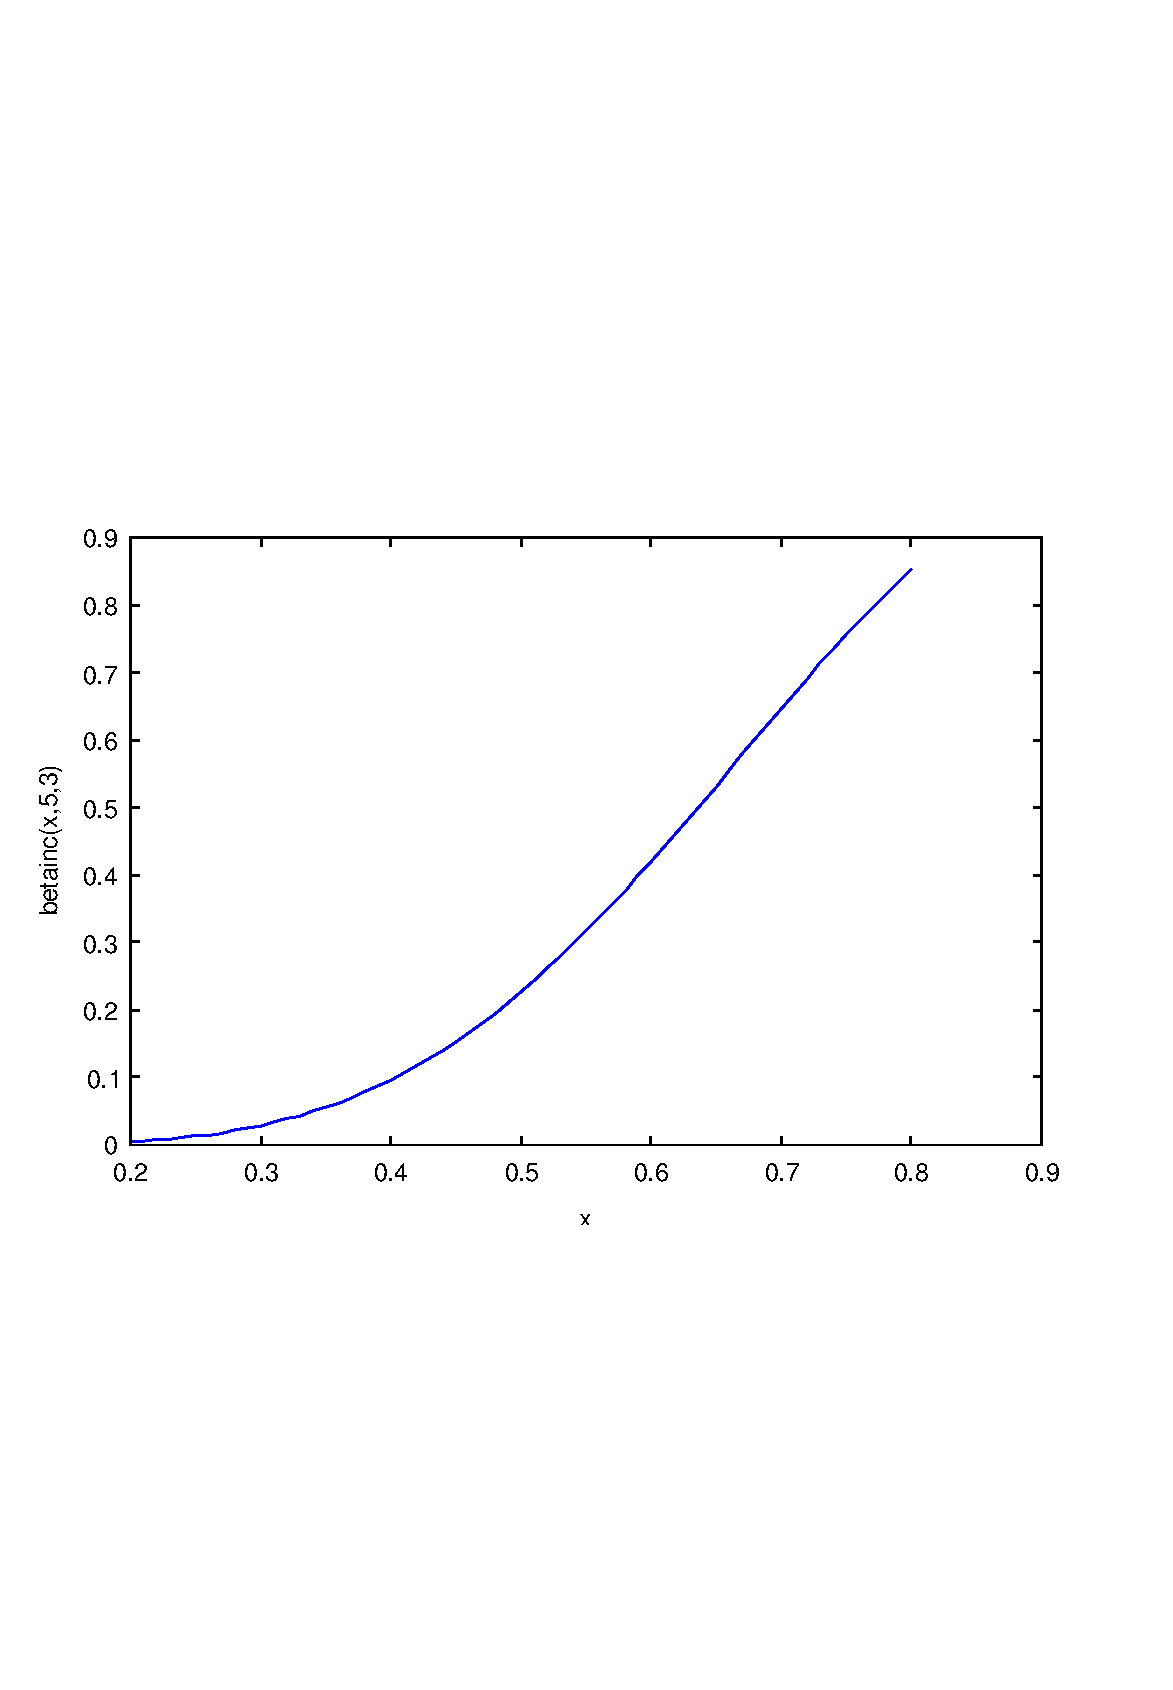
\includegraphics[width=12cm]{betainc1}
\caption{betainc1}
\end{DoxyImage}
 \hypertarget{mathfunctions_cos}{}\section{C\-O\-S Trigonometric Cosine Function}\label{mathfunctions_cos}
Section\-: \hyperlink{sec_mathfunctions}{Mathematical Functions} \hypertarget{vtkwidgets_vtkxyplotwidget_Usage}{}\subsection{Usage}\label{vtkwidgets_vtkxyplotwidget_Usage}
Computes the {\ttfamily cos} function for its argument. The general syntax for its use is \begin{DoxyVerb}  y = cos(x)
\end{DoxyVerb}
 where {\ttfamily x} is an {\ttfamily n}-\/dimensional array of numerical type. Integer types are promoted to the {\ttfamily double} type prior to calculation of the {\ttfamily cos} function. Output {\ttfamily y} is of the same size and type as the input {\ttfamily x}, (unless {\ttfamily x} is an integer, in which case {\ttfamily y} is a {\ttfamily double} type). \hypertarget{transforms_svd_Function}{}\subsection{Internals}\label{transforms_svd_Function}
Mathematically, the {\ttfamily cos} function is defined for all real valued arguments {\ttfamily x} by the infinite summation \[ \cos x \equiv \sum_{n=0}^{\infty} \frac{(-1)^n x^{2n}}{(2n)!}. \] For complex valued arguments {\ttfamily z}, the cosine is computed via \[ \cos z \equiv \cos \Re z \cosh \Im z - \sin \Re z \sinh \Im z. \] \hypertarget{variables_struct_Example}{}\subsection{Example}\label{variables_struct_Example}
The following piece of code plots the real-\/valued {\ttfamily cos(2 pi x)} function over one period of {\ttfamily \mbox{[}0,1\mbox{]}}\-:


\begin{DoxyVerbInclude}
--> x = linspace(0,1);
--> plot(x,cos(2*pi*x))
\end{DoxyVerbInclude}


 
\begin{DoxyImage}
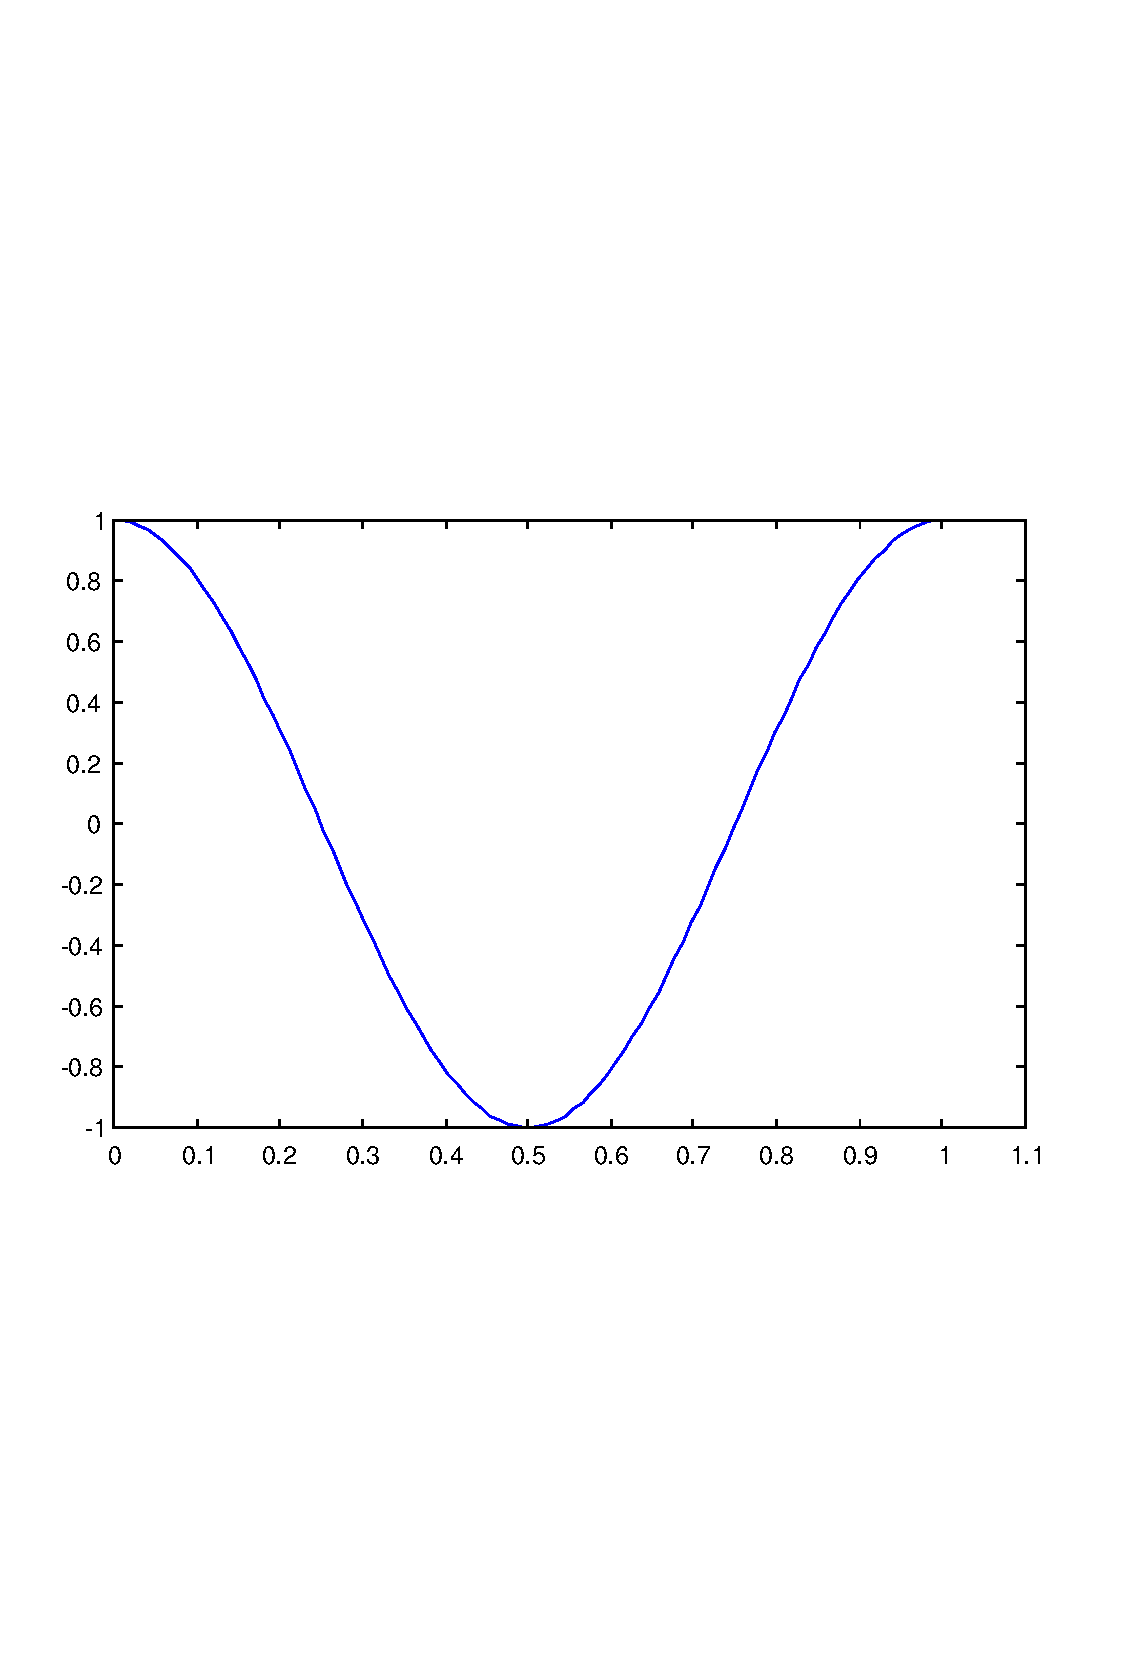
\includegraphics[width=12cm]{cosplot}
\caption{cosplot}
\end{DoxyImage}
 \hypertarget{mathfunctions_cosd}{}\section{C\-O\-S\-D Cosine Degrees Function}\label{mathfunctions_cosd}
Section\-: \hyperlink{sec_mathfunctions}{Mathematical Functions} \hypertarget{vtkwidgets_vtkxyplotwidget_Usage}{}\subsection{Usage}\label{vtkwidgets_vtkxyplotwidget_Usage}
Computes the cosine of the argument, but takes the argument in degrees instead of radians (as is the case for {\ttfamily cos}). The syntax for its use is \begin{DoxyVerb}   y = cosd(x)
\end{DoxyVerb}
 \hypertarget{variables_matrix_Examples}{}\subsection{Examples}\label{variables_matrix_Examples}
The cosine of 45 degrees should be {\ttfamily sqrt(2)/2}


\begin{DoxyVerbInclude}
--> cosd(45)

ans = 
    0.7071 
\end{DoxyVerbInclude}


and the cosine of {\ttfamily 60} degrees should be 0.\-5\-:


\begin{DoxyVerbInclude}
--> cosd(60)

ans = 
    0.5000 
\end{DoxyVerbInclude}
 \hypertarget{mathfunctions_cosh}{}\section{C\-O\-S\-H Hyperbolic Cosine Function}\label{mathfunctions_cosh}
Section\-: \hyperlink{sec_mathfunctions}{Mathematical Functions} \hypertarget{vtkwidgets_vtkxyplotwidget_Usage}{}\subsection{Usage}\label{vtkwidgets_vtkxyplotwidget_Usage}
Computes the hyperbolic cosine of the argument. The syntax for its use is \begin{DoxyVerb}   y = cosh(x)
\end{DoxyVerb}
 \hypertarget{transforms_svd_Function}{}\subsection{Internals}\label{transforms_svd_Function}
The {\ttfamily cosh} function is computed from the formula \[ \cosh(x) = \frac{e^x+e^{-x}}{2} \] For {\ttfamily x} complex, it follows that \[ \cosh(a+i*b) = \frac{e^a(\cos(b)+i*\sin(b)) + e^{-a}(\cos(-b)+i*\sin(-b))}{2} \] \hypertarget{variables_matrix_Examples}{}\subsection{Examples}\label{variables_matrix_Examples}
Here is a simple plot of the hyperbolic cosine function


\begin{DoxyVerbInclude}
--> x = linspace(-5,5);
--> plot(x,cosh(x)); grid('on');
\end{DoxyVerbInclude}


 
\begin{DoxyImage}
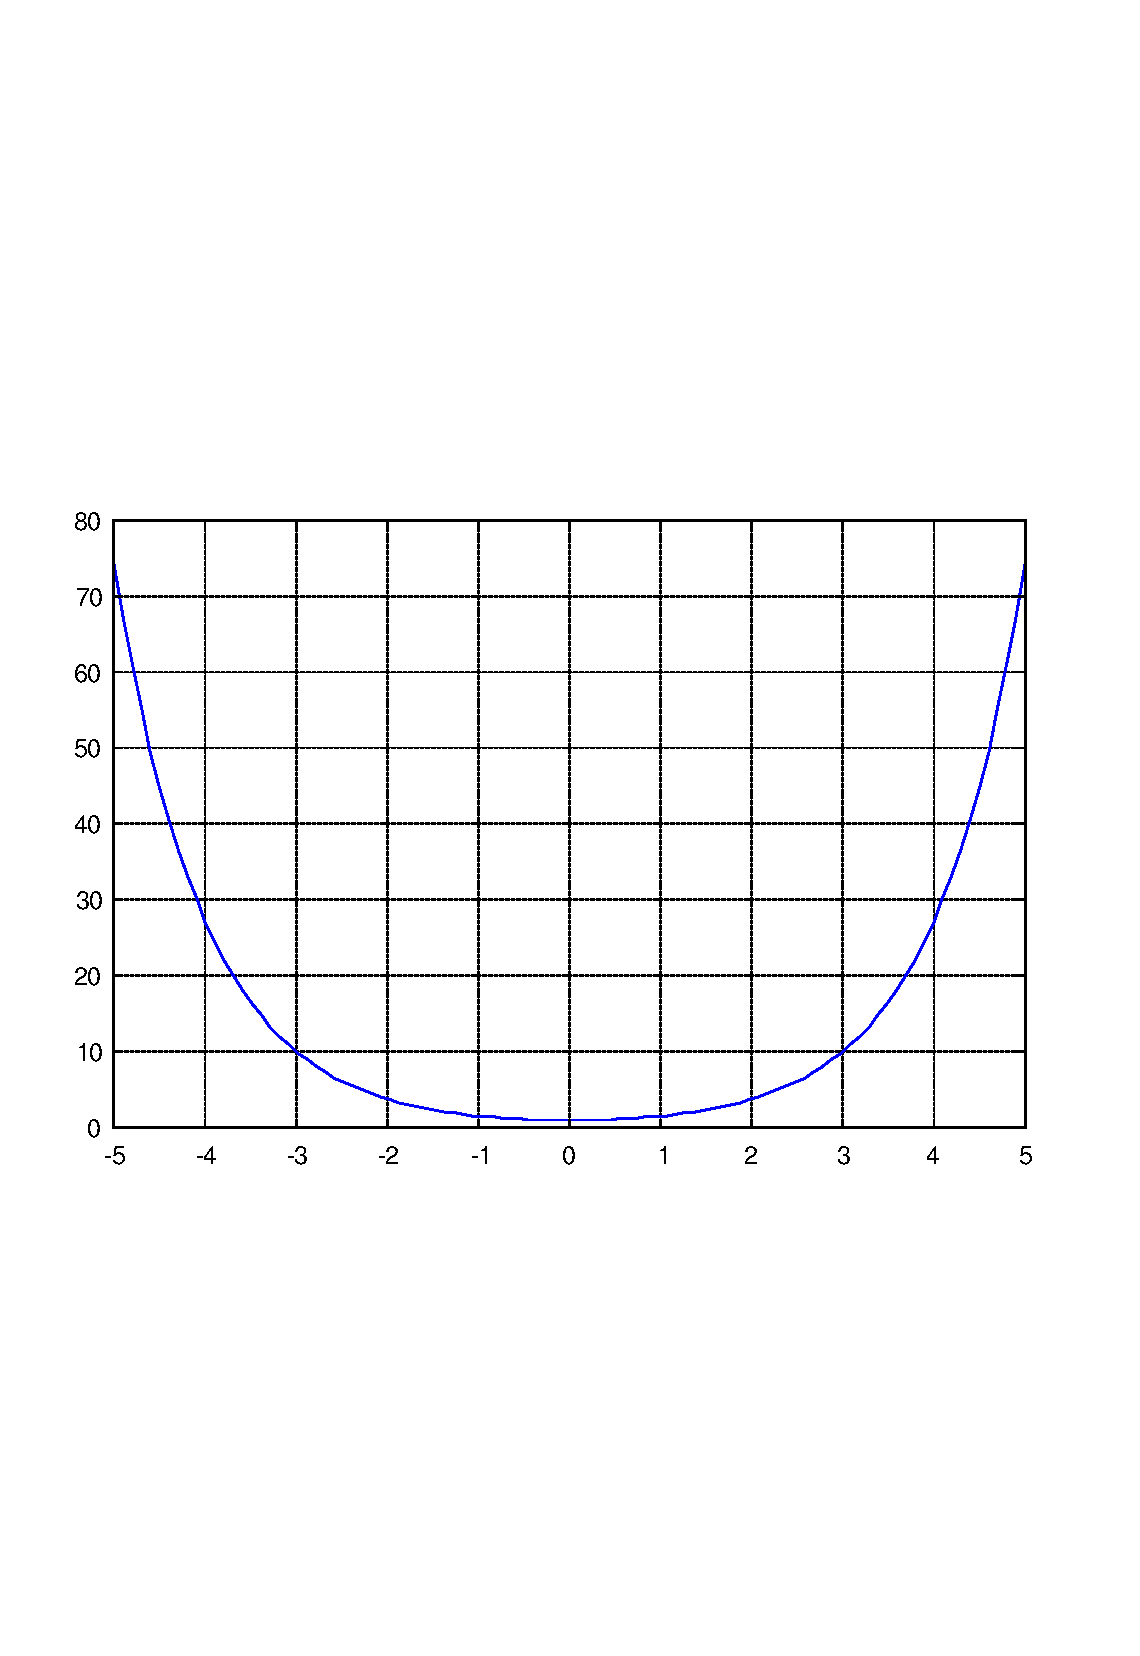
\includegraphics[width=12cm]{coshplot}
\caption{coshplot}
\end{DoxyImage}
 \hypertarget{mathfunctions_cot}{}\section{C\-O\-T Trigonometric Cotangent Function}\label{mathfunctions_cot}
Section\-: \hyperlink{sec_mathfunctions}{Mathematical Functions} \hypertarget{vtkwidgets_vtkxyplotwidget_Usage}{}\subsection{Usage}\label{vtkwidgets_vtkxyplotwidget_Usage}
Computes the {\ttfamily cot} function for its argument. The general syntax for its use is \begin{DoxyVerb}  y = cot(x)
\end{DoxyVerb}
 where {\ttfamily x} is an {\ttfamily n}-\/dimensional array of numerical type. Integer types are promoted to the {\ttfamily double} type prior to calculation of the {\ttfamily cot} function. Output {\ttfamily y} is of the same size and type as the input {\ttfamily x}, (unless {\ttfamily x} is an integer, in which case {\ttfamily y} is a {\ttfamily double} type). \hypertarget{transforms_svd_Function}{}\subsection{Internals}\label{transforms_svd_Function}
Mathematically, the {\ttfamily cot} function is defined for all arguments {\ttfamily x} as \[ \cot x \equiv \frac{\cos x}{\sin x} \] For complex valued arguments {\ttfamily z}, the cotangent is computed via \[ \cot z \equiv \frac{\cos 2 \Re z + \cosh 2 \Im z}{\sin 2 \Re z + i \sinh 2 \Im z}. \] \hypertarget{variables_struct_Example}{}\subsection{Example}\label{variables_struct_Example}
The following piece of code plots the real-\/valued {\ttfamily cot(x)} function over the interval {\ttfamily \mbox{[}-\/1,1\mbox{]}}\-:


\begin{DoxyVerbInclude}
--> t = linspace(-1,1);
--> plot(t,cot(t))
\end{DoxyVerbInclude}


 
\begin{DoxyImage}
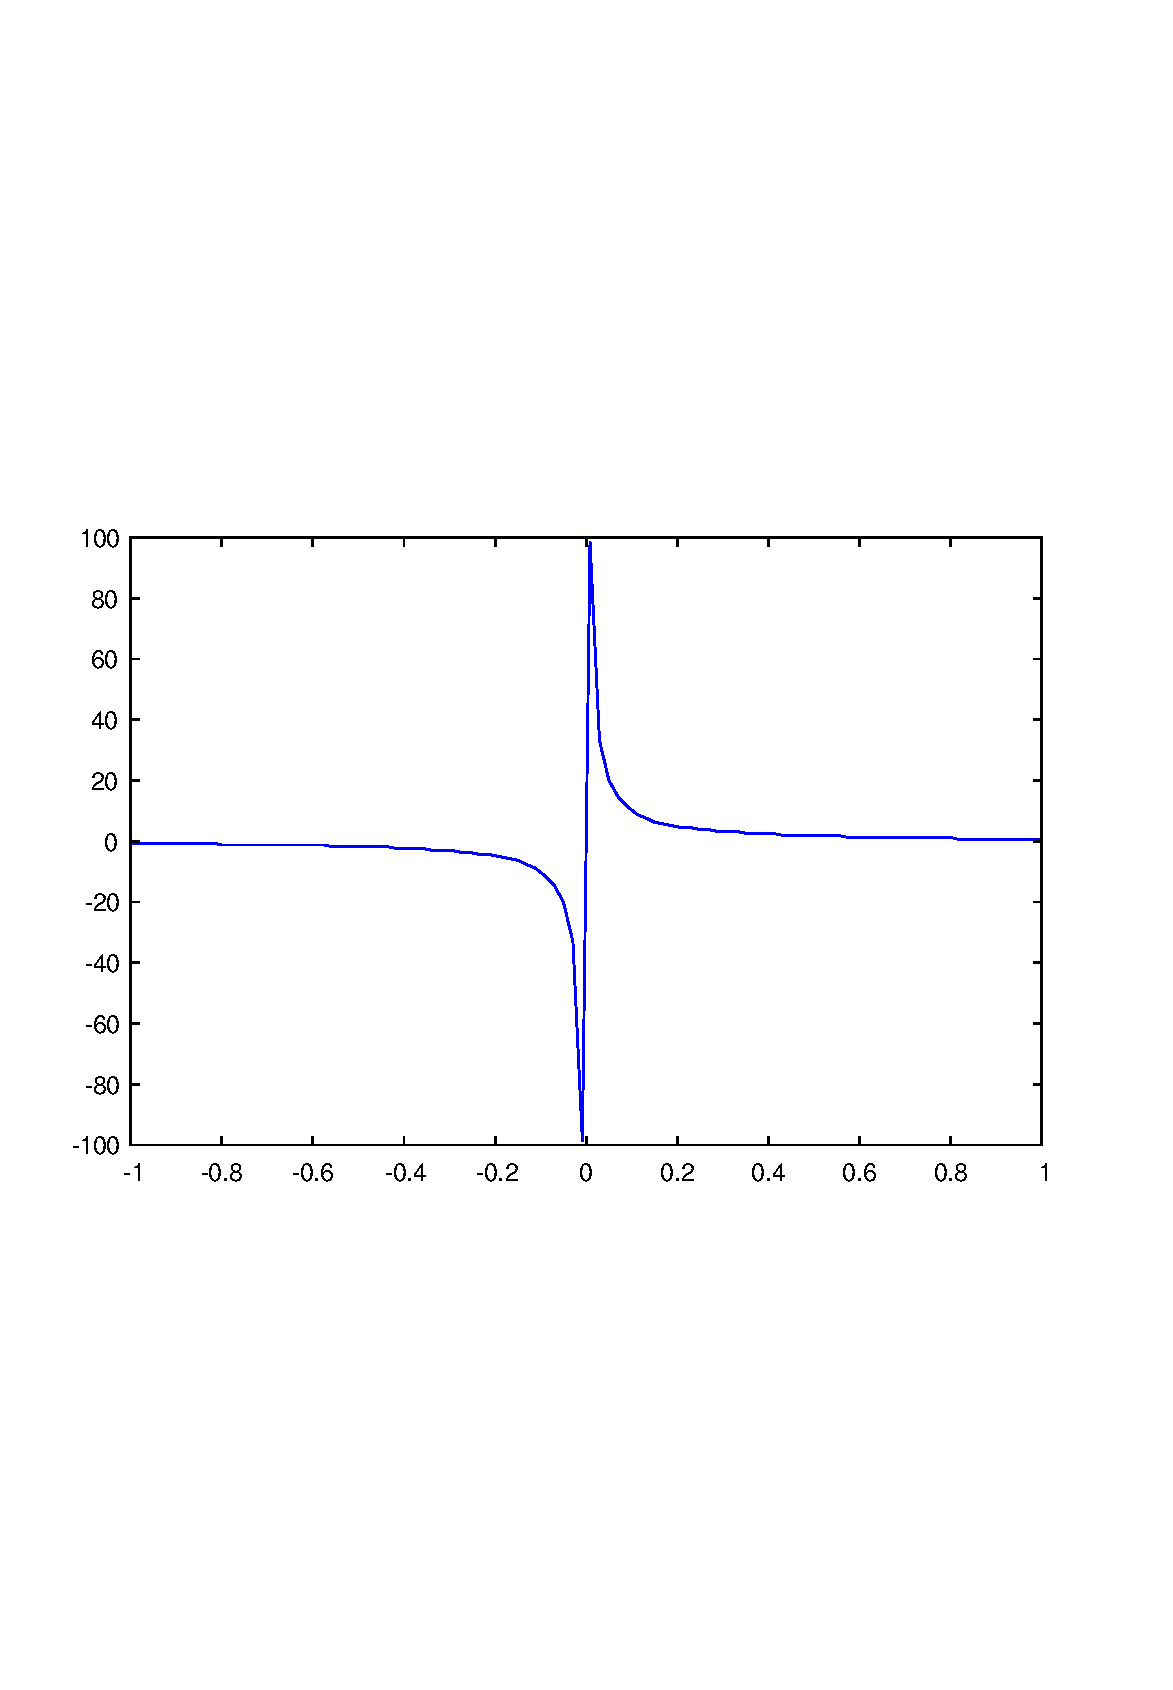
\includegraphics[width=12cm]{cotplot}
\caption{cotplot}
\end{DoxyImage}
 \hypertarget{mathfunctions_cotd}{}\section{C\-O\-T\-D Cotangent Degrees Function}\label{mathfunctions_cotd}
Section\-: \hyperlink{sec_mathfunctions}{Mathematical Functions} \hypertarget{vtkwidgets_vtkxyplotwidget_Usage}{}\subsection{Usage}\label{vtkwidgets_vtkxyplotwidget_Usage}
Computes the cotangent of the argument, but takes the argument in degrees instead of radians (as is the case for {\ttfamily cot}). The syntax for its use is \begin{DoxyVerb}   y = cotd(x)
\end{DoxyVerb}
 \hypertarget{variables_matrix_Examples}{}\subsection{Examples}\label{variables_matrix_Examples}
The cotangent of 45 degrees should be 1.


\begin{DoxyVerbInclude}
--> cotd(45)

ans = 
    1.0000 
\end{DoxyVerbInclude}
 \hypertarget{mathfunctions_coth}{}\section{C\-O\-T\-H Hyperbolic Cotangent Function}\label{mathfunctions_coth}
Section\-: \hyperlink{sec_mathfunctions}{Mathematical Functions} \hypertarget{vtkwidgets_vtkxyplotwidget_Usage}{}\subsection{Usage}\label{vtkwidgets_vtkxyplotwidget_Usage}
Computes the hyperbolic cotangent of the argument. The syntax for its use is \begin{DoxyVerb}   y = coth(x)
\end{DoxyVerb}
 \hypertarget{transforms_svd_Function}{}\subsection{Internals}\label{transforms_svd_Function}
The {\ttfamily coth} function is computed from the formula \[ \coth(x) = \frac{1}{\tanh(x)} \] \hypertarget{variables_matrix_Examples}{}\subsection{Examples}\label{variables_matrix_Examples}
Here is a simple plot of the hyperbolic cotangent function


\begin{DoxyVerbInclude}
--> x1 = -pi+.01:.01:-.01;
--> x2 = .01:.01:pi-.01;
--> plot(x1,coth(x1),x2,coth(x2)); grid('on');
\end{DoxyVerbInclude}


 
\begin{DoxyImage}
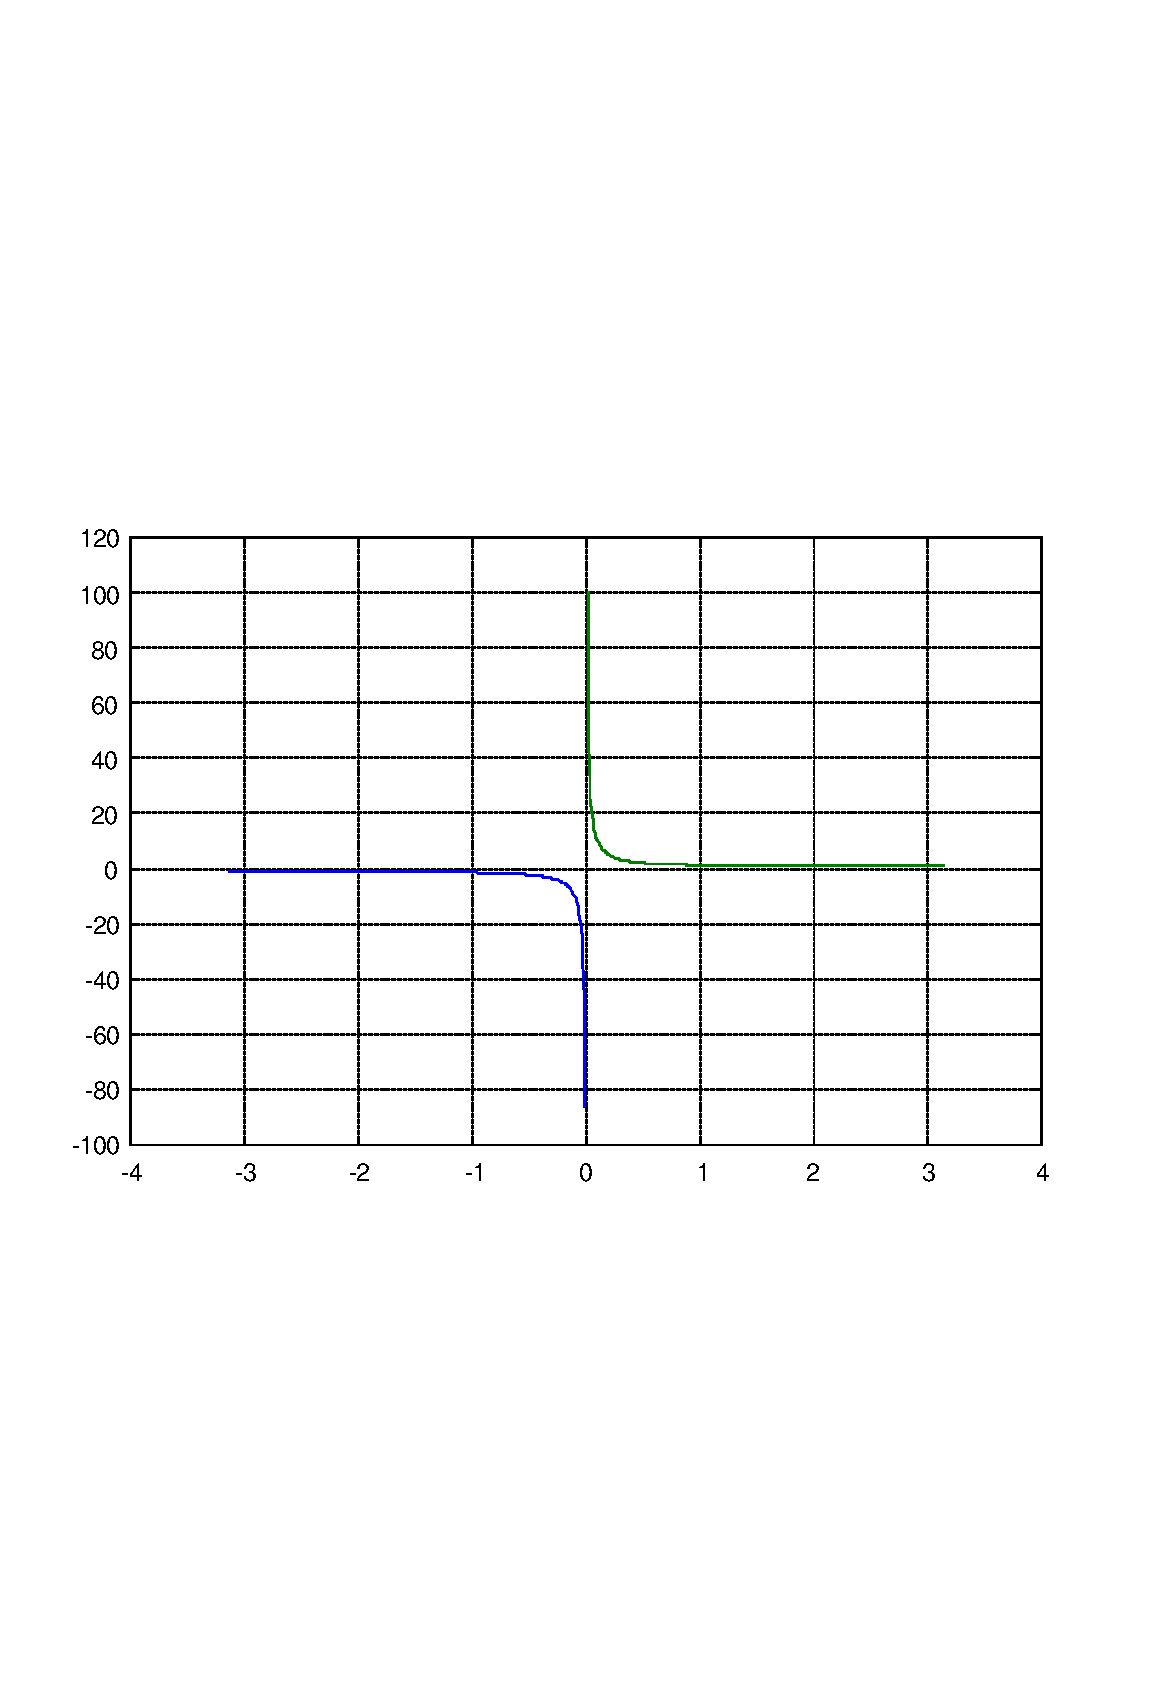
\includegraphics[width=12cm]{cothplot}
\caption{cothplot}
\end{DoxyImage}
 \hypertarget{mathfunctions_cross}{}\section{C\-R\-O\-S\-S Cross Product of Two Vectors}\label{mathfunctions_cross}
Section\-: \hyperlink{sec_mathfunctions}{Mathematical Functions} \hypertarget{vtkwidgets_vtkxyplotwidget_Usage}{}\subsection{Usage}\label{vtkwidgets_vtkxyplotwidget_Usage}
Computes the cross product of two vectors. The general syntax for its use is \begin{DoxyVerb}    c = cross(a,b)
\end{DoxyVerb}
 where {\ttfamily a} and {\ttfamily b} are 3-\/element vectors. \hypertarget{mathfunctions_csc}{}\section{C\-S\-C Trigonometric Cosecant Function}\label{mathfunctions_csc}
Section\-: \hyperlink{sec_mathfunctions}{Mathematical Functions} \hypertarget{vtkwidgets_vtkxyplotwidget_Usage}{}\subsection{Usage}\label{vtkwidgets_vtkxyplotwidget_Usage}
Computes the {\ttfamily csc} function for its argument. The general syntax for its use is \begin{DoxyVerb}  y = csc(x)
\end{DoxyVerb}
 where {\ttfamily x} is an {\ttfamily n}-\/dimensional array of numerical type. Integer types are promoted to the {\ttfamily double} type prior to calculation of the {\ttfamily csc} function. Output {\ttfamily y} is of the same size and type as the input {\ttfamily x}, (unless {\ttfamily x} is an integer, in which case {\ttfamily y} is a {\ttfamily double} type). \hypertarget{transforms_svd_Function}{}\subsection{Internals}\label{transforms_svd_Function}
Mathematically, the {\ttfamily csc} function is defined for all arguments as \[ \csc x \equiv \frac{1}{\sin x}. \] \hypertarget{variables_struct_Example}{}\subsection{Example}\label{variables_struct_Example}
The following piece of code plots the real-\/valued {\ttfamily csc(2 pi x)} function over the interval of {\ttfamily \mbox{[}-\/1,1\mbox{]}}\-:


\begin{DoxyVerbInclude}
--> t = linspace(-1,1,1000);
--> plot(t,csc(2*pi*t))
--> axis([-1,1,-10,10]);
\end{DoxyVerbInclude}


 
\begin{DoxyImage}
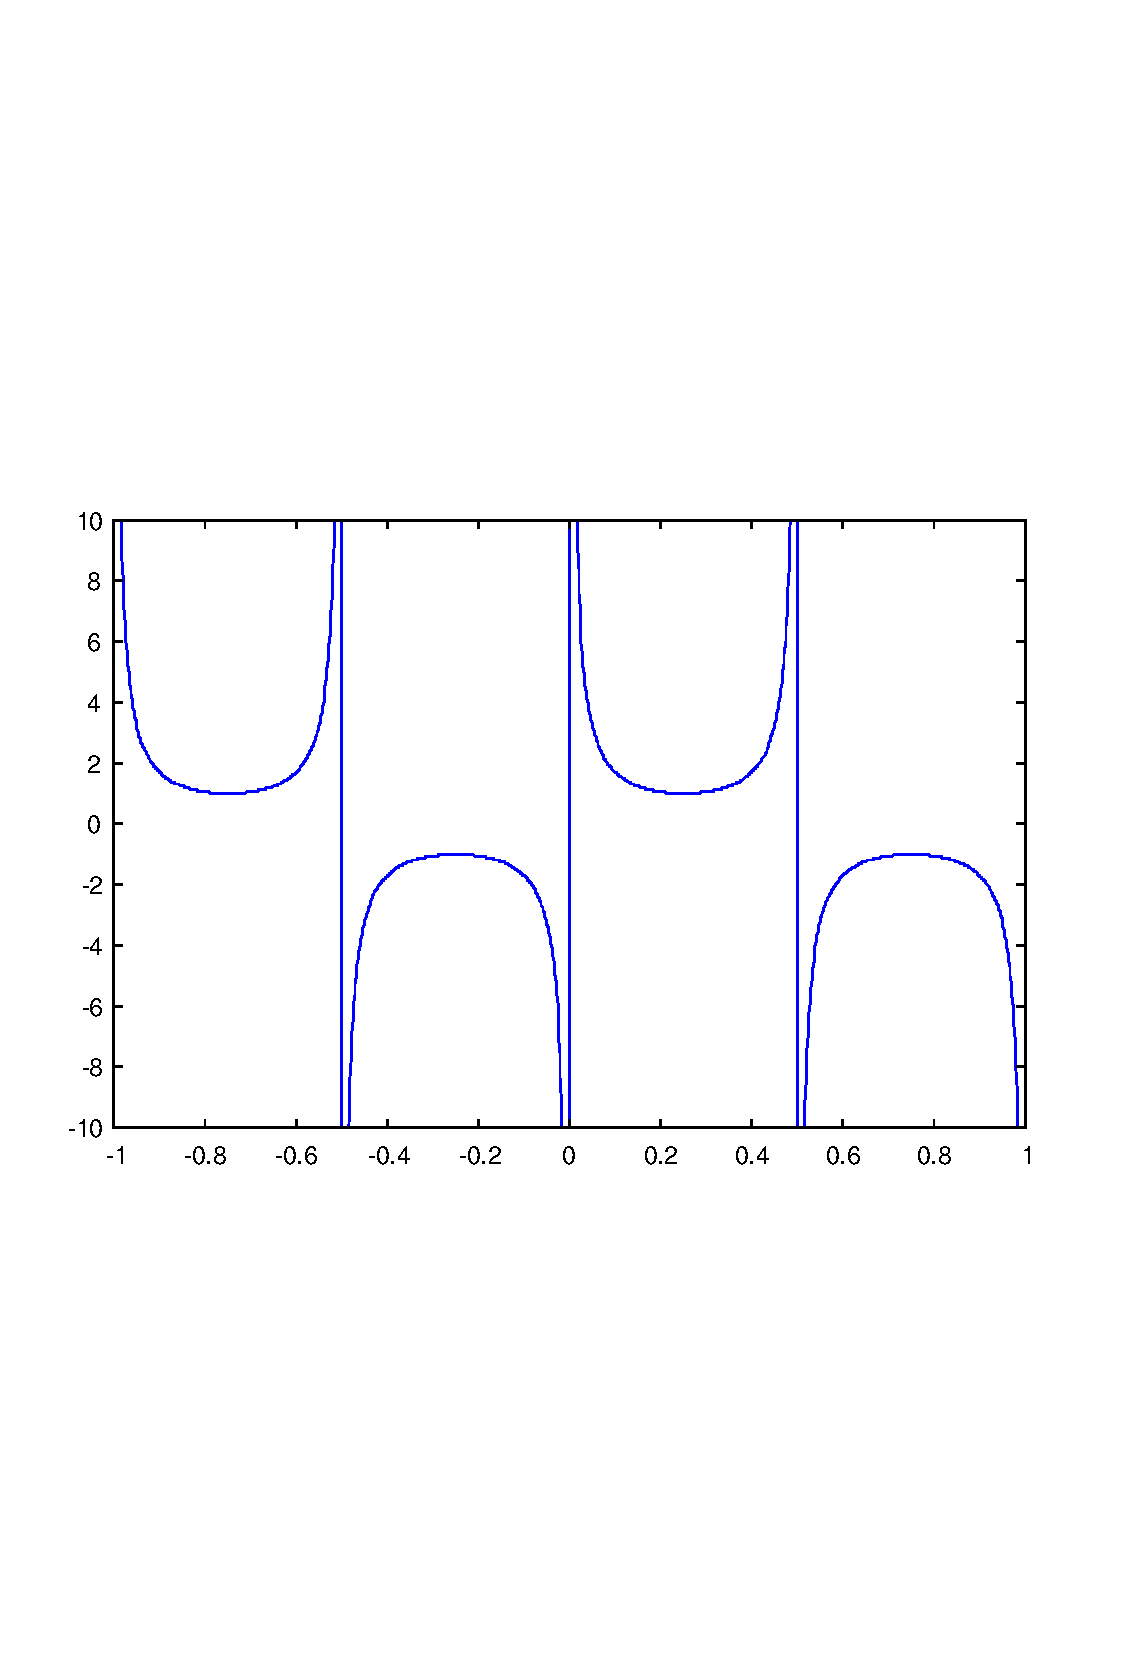
\includegraphics[width=12cm]{cscplot}
\caption{cscplot}
\end{DoxyImage}
 \hypertarget{mathfunctions_cscd}{}\section{C\-S\-C\-D Cosecant Degrees Function}\label{mathfunctions_cscd}
Section\-: \hyperlink{sec_mathfunctions}{Mathematical Functions} \hypertarget{vtkwidgets_vtkxyplotwidget_Usage}{}\subsection{Usage}\label{vtkwidgets_vtkxyplotwidget_Usage}
Computes the cosecant of the argument, but takes the argument in degrees instead of radians (as is the case for {\ttfamily csc}). The syntax for its use is \begin{DoxyVerb}   y = cscd(x)
\end{DoxyVerb}
 \hypertarget{mathfunctions_csch}{}\section{C\-S\-C\-H Hyperbolic Cosecant Function}\label{mathfunctions_csch}
Section\-: \hyperlink{sec_mathfunctions}{Mathematical Functions} \hypertarget{vtkwidgets_vtkxyplotwidget_Usage}{}\subsection{Usage}\label{vtkwidgets_vtkxyplotwidget_Usage}
Computes the hyperbolic cosecant of the argument. The syntax for its use is \begin{DoxyVerb}   y = csch(x)
\end{DoxyVerb}
 \hypertarget{transforms_svd_Function}{}\subsection{Internals}\label{transforms_svd_Function}
The {\ttfamily csch} function is computed from the formula \[ \mathrm{csch}(x) = \frac{1}{\sinh(x)} \] \hypertarget{variables_matrix_Examples}{}\subsection{Examples}\label{variables_matrix_Examples}
Here is a simple plot of the hyperbolic cosecant function


\begin{DoxyVerbInclude}
--> x1 = -pi+.01:.01:-.01;
--> x2 = .01:.01:pi-.01;
--> plot(x1,csch(x1),x2,csch(x2)); grid('on');
\end{DoxyVerbInclude}


 
\begin{DoxyImage}
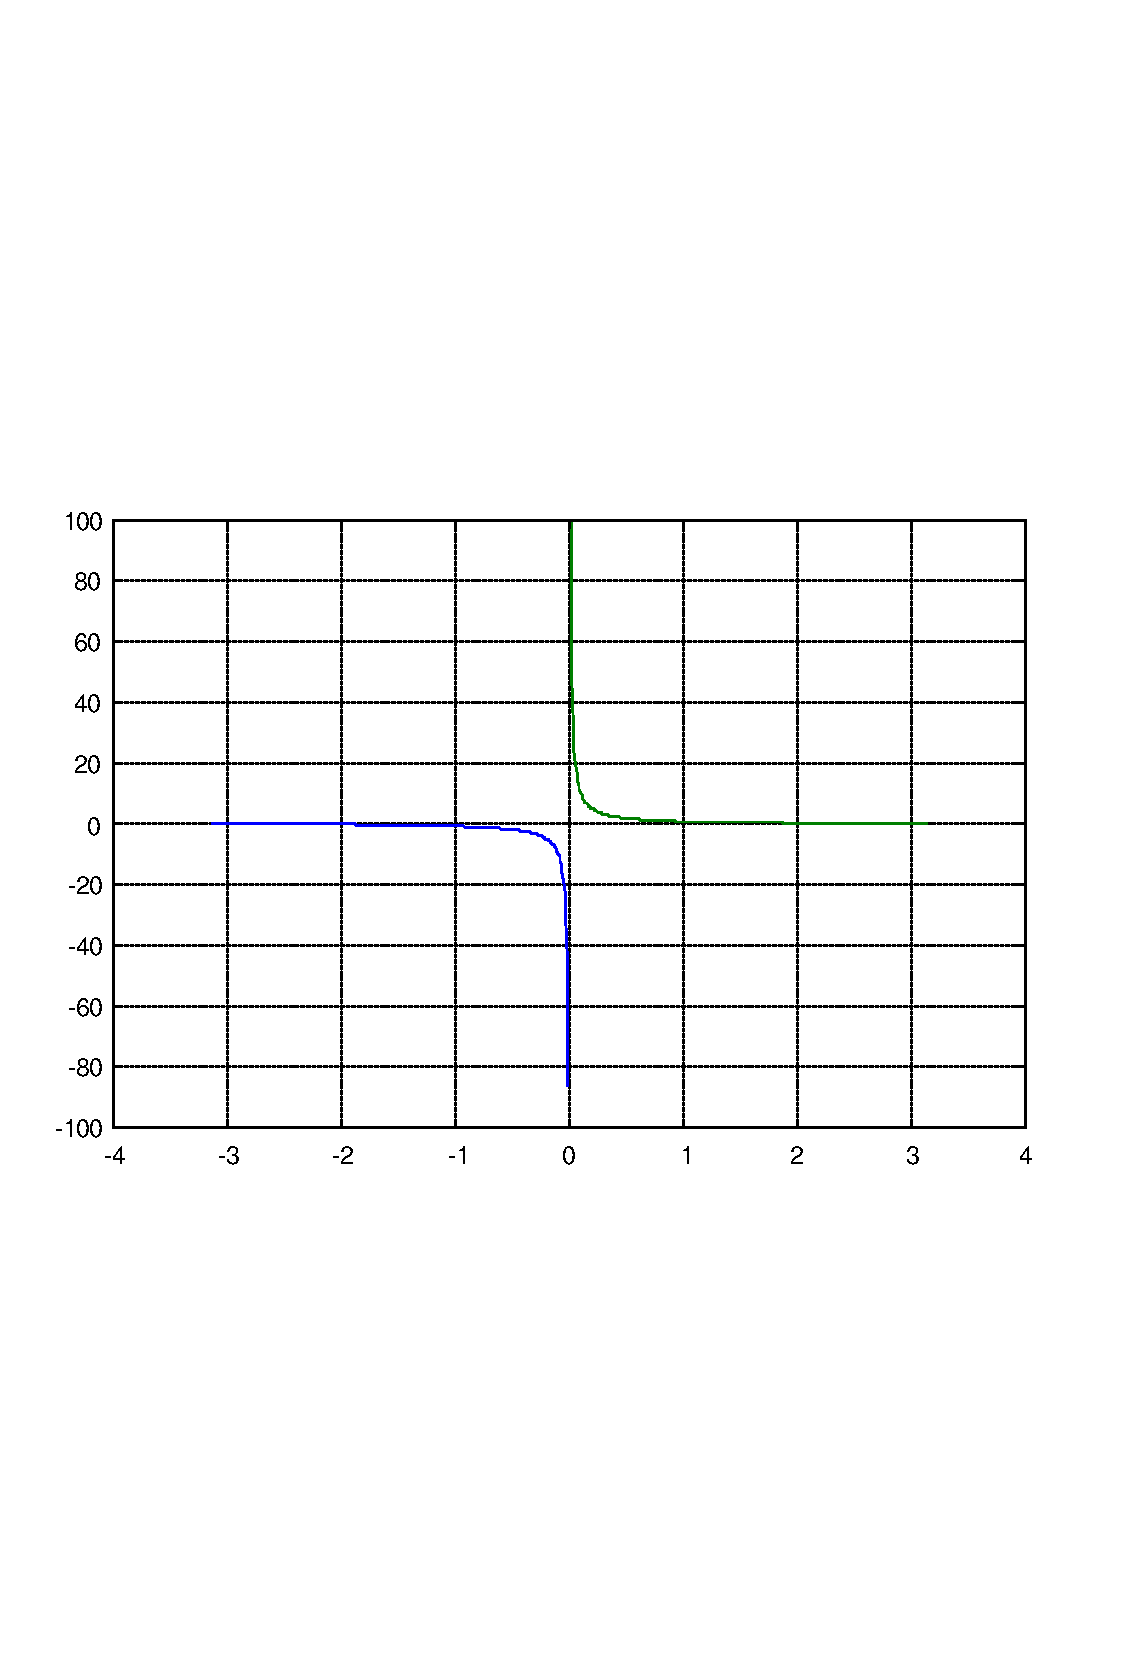
\includegraphics[width=12cm]{cschplot}
\caption{cschplot}
\end{DoxyImage}
 \hypertarget{mathfunctions_deg2rad}{}\section{D\-E\-G2\-R\-A\-D Convert From Degrees To Radians}\label{mathfunctions_deg2rad}
Section\-: \hyperlink{sec_mathfunctions}{Mathematical Functions} \hypertarget{vtkwidgets_vtkxyplotwidget_Usage}{}\subsection{Usage}\label{vtkwidgets_vtkxyplotwidget_Usage}
Converts the argument from degrees to radians. The syntax for its use is \begin{DoxyVerb}   y = deg2rad(x)
\end{DoxyVerb}
 where {\ttfamily x} is a numeric array. Conversion is done by simply multiplying {\ttfamily x} by {\ttfamily pi/180}. \hypertarget{variables_struct_Example}{}\subsection{Example}\label{variables_struct_Example}
How many radians in a circle\-:


\begin{DoxyVerbInclude}
--> deg2rad(360) - 2*pi

ans = 
 0 
\end{DoxyVerbInclude}
 \hypertarget{mathfunctions_erf}{}\section{E\-R\-F Error Function}\label{mathfunctions_erf}
Section\-: \hyperlink{sec_mathfunctions}{Mathematical Functions} \hypertarget{vtkwidgets_vtkxyplotwidget_Usage}{}\subsection{Usage}\label{vtkwidgets_vtkxyplotwidget_Usage}
Computes the error function for real arguments. The {\ttfamily erf} function takes only a single argument \begin{DoxyVerb}  y = erf(x)
\end{DoxyVerb}
 where {\ttfamily x} is either a {\ttfamily float} or {\ttfamily double} array. The output vector {\ttfamily y} is the same size (and type) as {\ttfamily x}. \hypertarget{transforms_svd_Function}{}\subsection{Internals}\label{transforms_svd_Function}
The erf function is defined by the integral\-: \[ \mathrm{erf}(x) = \frac{2}{\sqrt{\pi}}\int_{0}^{x} e^{-t^2} \, dt, \] and is the integral of the normal distribution. \hypertarget{variables_struct_Example}{}\subsection{Example}\label{variables_struct_Example}
Here is a plot of the erf function over the range {\ttfamily \mbox{[}-\/5,5\mbox{]}}.


\begin{DoxyVerbInclude}
--> x = linspace(-5,5);
--> y = erf(x);
--> plot(x,y); xlabel('x'); ylabel('erf(x)');
\end{DoxyVerbInclude}


which results in the following plot.  
\begin{DoxyImage}
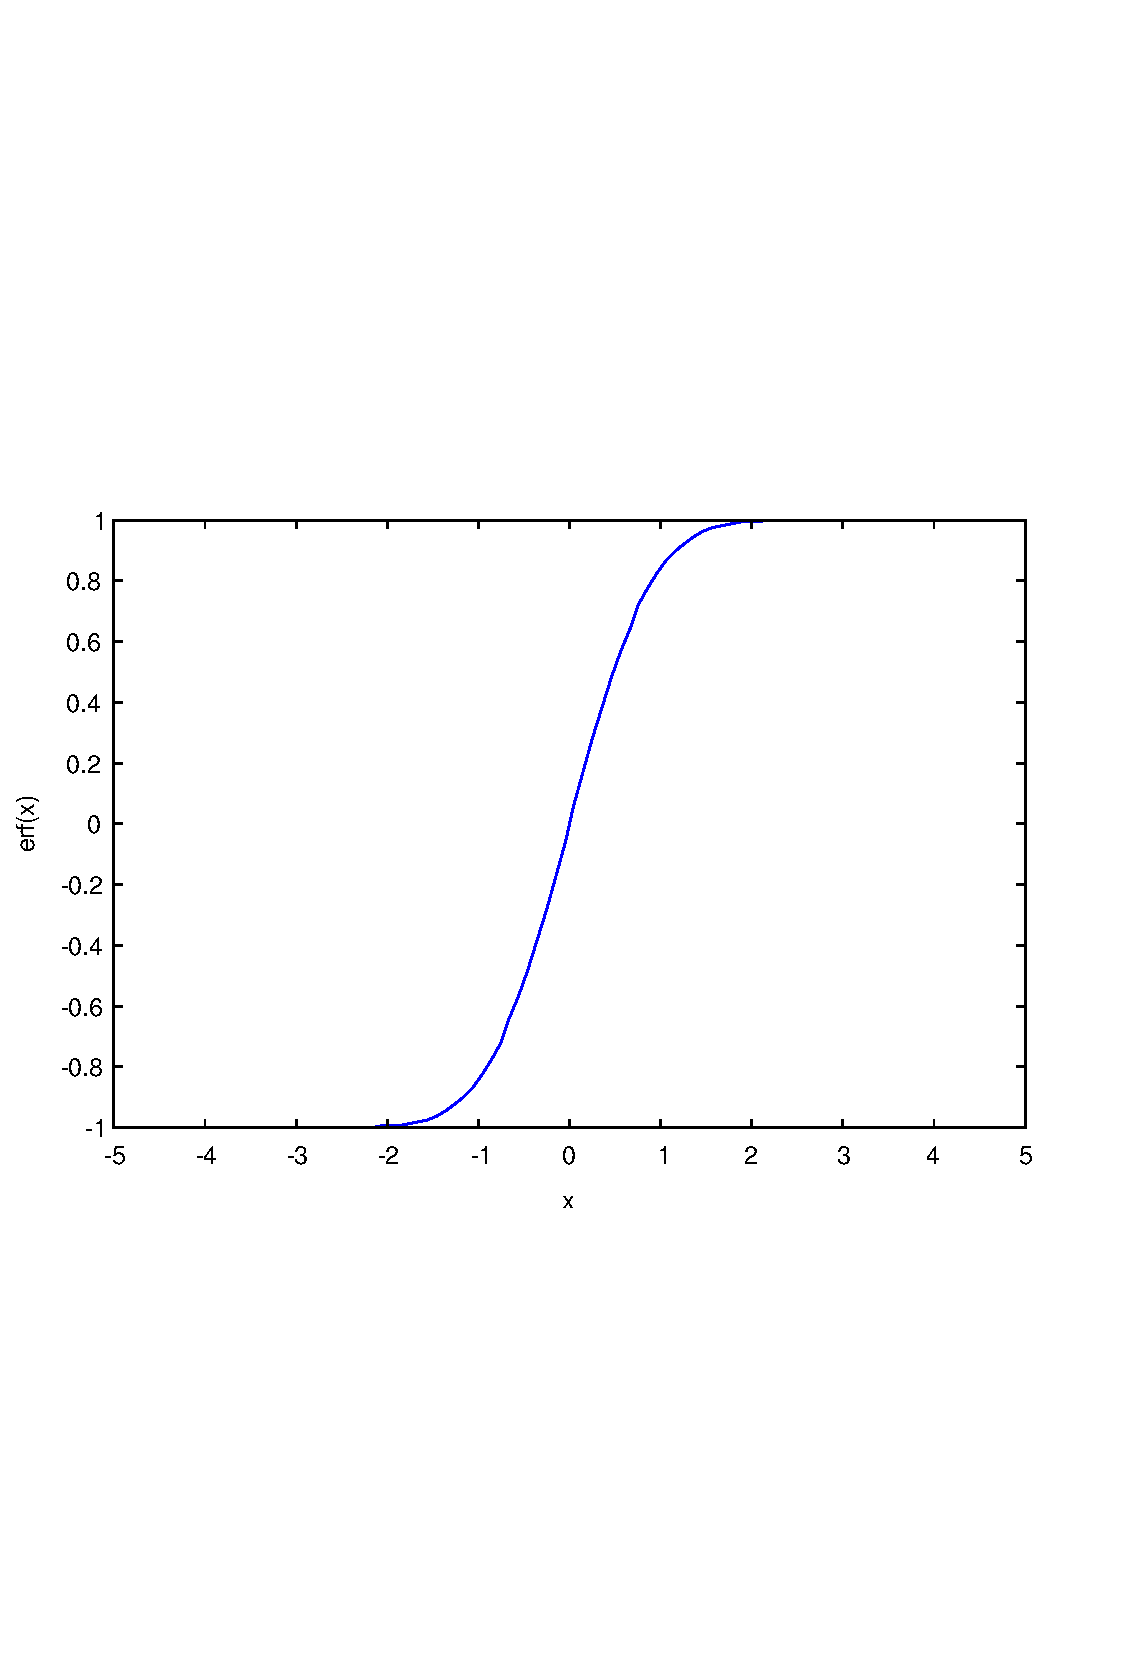
\includegraphics[width=12cm]{erf1}
\caption{erf1}
\end{DoxyImage}
 \hypertarget{mathfunctions_erfc}{}\section{E\-R\-F\-C Complimentary Error Function}\label{mathfunctions_erfc}
Section\-: \hyperlink{sec_mathfunctions}{Mathematical Functions} \hypertarget{vtkwidgets_vtkxyplotwidget_Usage}{}\subsection{Usage}\label{vtkwidgets_vtkxyplotwidget_Usage}
Computes the complimentary error function for real arguments. The {\ttfamily erfc} function takes only a single argument \begin{DoxyVerb}  y = erfc(x)
\end{DoxyVerb}
 where {\ttfamily x} is either a {\ttfamily float} or {\ttfamily double} array. The output vector {\ttfamily y} is the same size (and type) as {\ttfamily x}. \hypertarget{transforms_svd_Function}{}\subsection{Internals}\label{transforms_svd_Function}
The erfc function is defined by the integral\-: \[ \mathrm{erfc}(x) = \frac{2}{\sqrt{\pi}}\int_{x}^{\infty} e^{-t^2} \, dt, \] and is the integral of the normal distribution. \hypertarget{variables_struct_Example}{}\subsection{Example}\label{variables_struct_Example}
Here is a plot of the {\ttfamily erfc} function over the range {\ttfamily \mbox{[}-\/5,5\mbox{]}}.


\begin{DoxyVerbInclude}
--> x = linspace(-5,5);
--> y = erfc(x);
--> plot(x,y); xlabel('x'); ylabel('erfc(x)');
\end{DoxyVerbInclude}


which results in the following plot.  
\begin{DoxyImage}
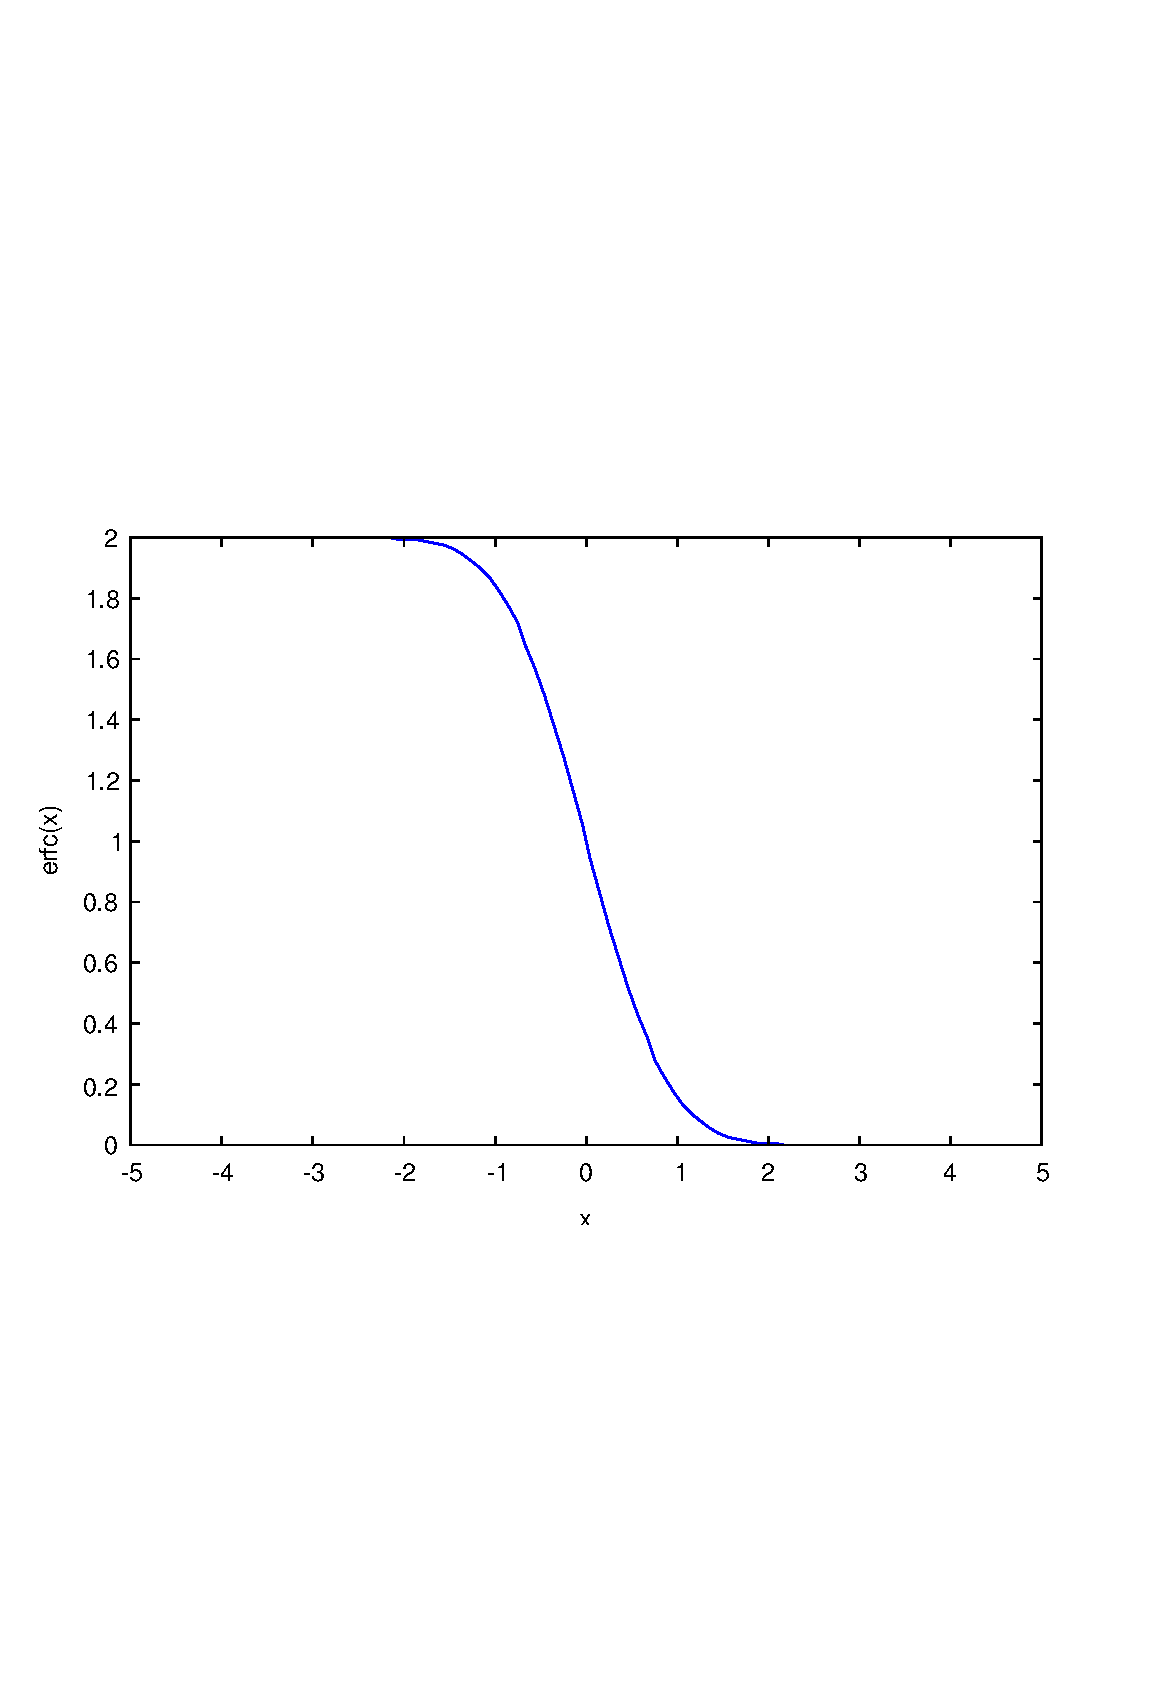
\includegraphics[width=12cm]{erfc1}
\caption{erfc1}
\end{DoxyImage}
 \hypertarget{mathfunctions_erfinv}{}\section{E\-R\-F\-I\-N\-V Inverse Error Function}\label{mathfunctions_erfinv}
Section\-: \hyperlink{sec_mathfunctions}{Mathematical Functions} \hypertarget{vtkwidgets_vtkxyplotwidget_Usage}{}\subsection{Usage}\label{vtkwidgets_vtkxyplotwidget_Usage}
Computes the inverse error function for each element of x. The {\ttfamily erf} function takes only a single argument \begin{DoxyVerb}  y = erfinv(x)
\end{DoxyVerb}
 where {\ttfamily x} is either a {\ttfamily float} or {\ttfamily double} array. The output vector {\ttfamily y} is the same size (and type) as {\ttfamily x}. For values outside the interval \mbox{[}-\/1, 1\mbox{]} function returns Na\-N. \hypertarget{variables_struct_Example}{}\subsection{Example}\label{variables_struct_Example}
Here is a plot of the erf function over the range {\ttfamily \mbox{[}-\/.\-9,.9\mbox{]}}.


\begin{DoxyVerbInclude}
--> x = linspace(-.9,.9,100);
--> y = erfinv(x);
--> plot(x,y); xlabel('x'); ylabel('erfinv(x)');
\end{DoxyVerbInclude}


which results in the following plot.  
\begin{DoxyImage}
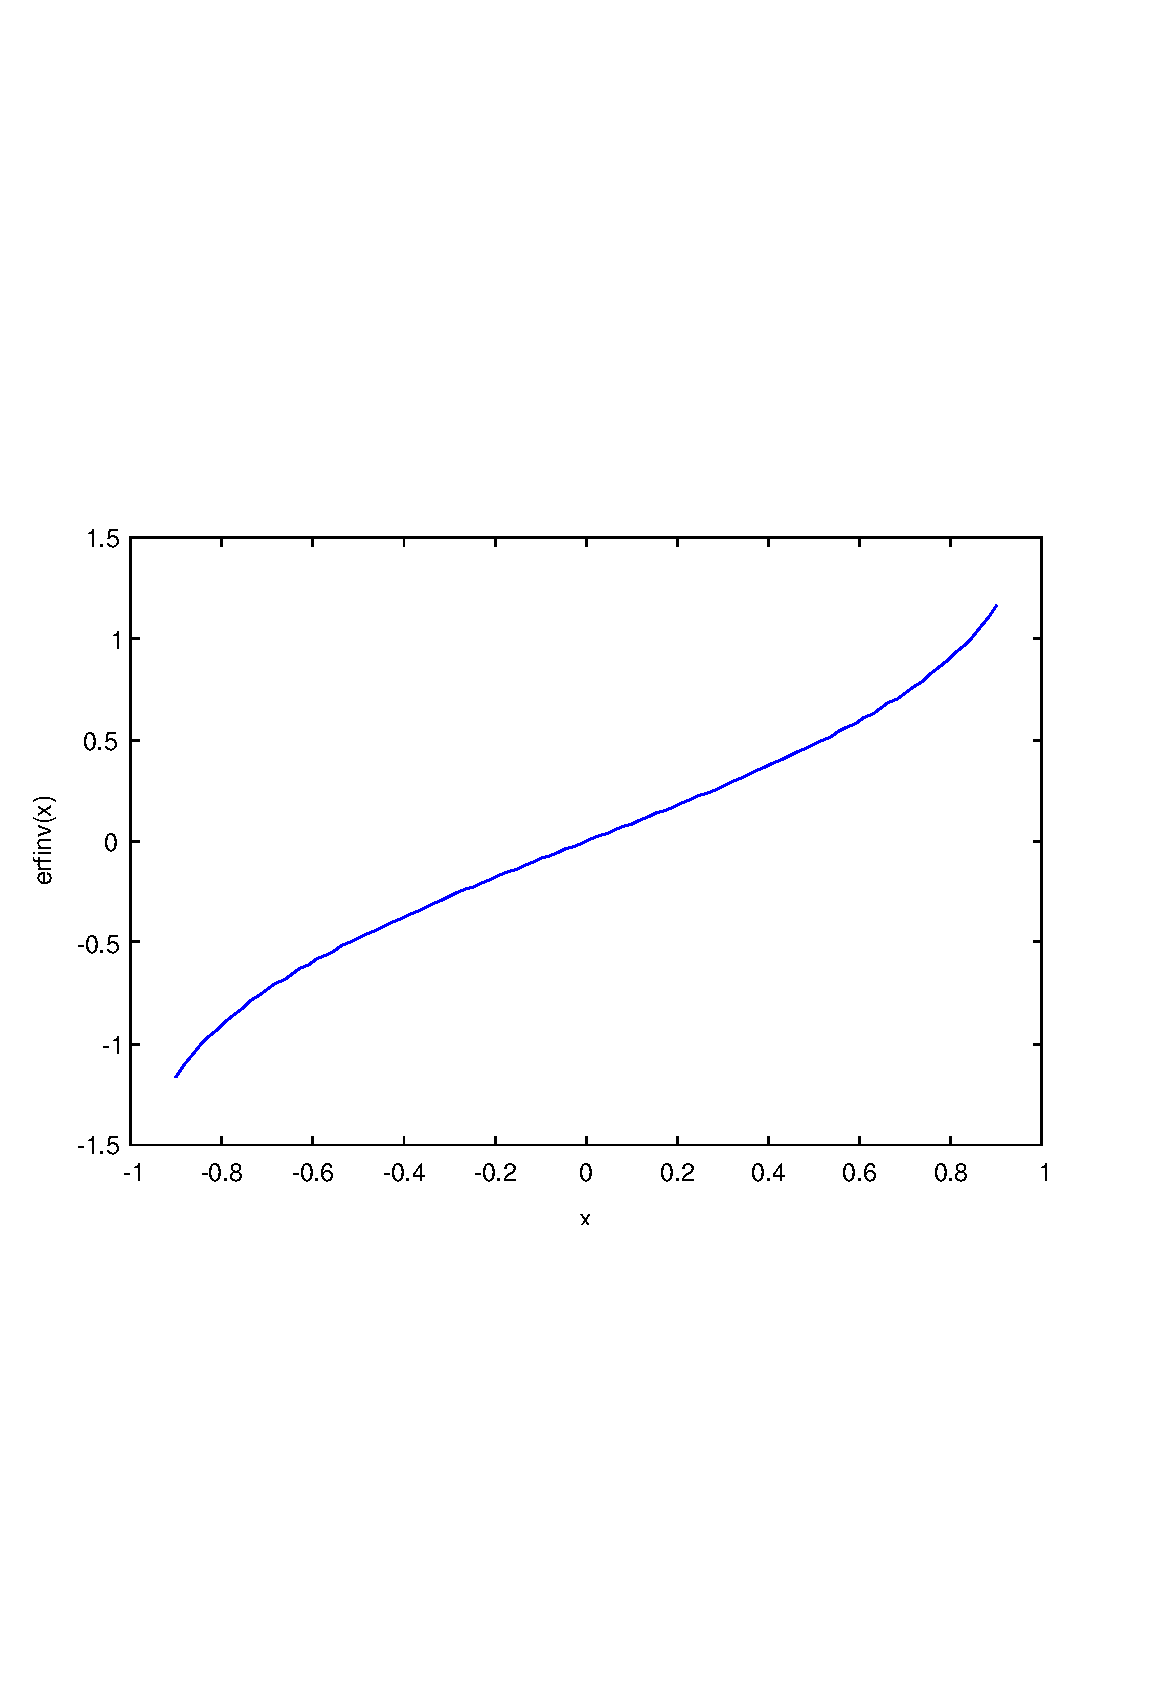
\includegraphics[width=12cm]{erfinv1}
\caption{erfinv1}
\end{DoxyImage}
 \hypertarget{mathfunctions_exp}{}\section{E\-X\-P Exponential Function}\label{mathfunctions_exp}
Section\-: \hyperlink{sec_mathfunctions}{Mathematical Functions} \hypertarget{vtkwidgets_vtkxyplotwidget_Usage}{}\subsection{Usage}\label{vtkwidgets_vtkxyplotwidget_Usage}
Computes the {\ttfamily exp} function for its argument. The general syntax for its use is \begin{DoxyVerb}   y = exp(x)
\end{DoxyVerb}
 where {\ttfamily x} is an {\ttfamily n}-\/dimensional array of numerical type. Integer types are promoted to the {\ttfamily double} type prior to calculation of the {\ttfamily exp} function. Output {\ttfamily y} is of the same size and type as the input {\ttfamily x}, (unless {\ttfamily x} is an integer, in which case {\ttfamily y} is a {\ttfamily double} type). \hypertarget{transforms_svd_Function}{}\subsection{Internals}\label{transforms_svd_Function}
Mathematically, the {\ttfamily exp} function is defined for all real valued arguments {\ttfamily x} as \[ \exp x \equiv e^{x}, \] where \[ e = \sum_{0}^{\infty} \frac{1}{k!} \] and is approximately {\ttfamily 2.\-718281828459045} (returned by the function {\ttfamily e}). For complex values {\ttfamily z}, the famous Euler formula is used to calculate the exponential \[ e^{z} = e^{|z|} \left[ \cos \Re z + i \sin \Re z \right] \] \hypertarget{variables_struct_Example}{}\subsection{Example}\label{variables_struct_Example}
The following piece of code plots the real-\/valued {\ttfamily exp} function over the interval {\ttfamily \mbox{[}-\/1,1\mbox{]}}\-:


\begin{DoxyVerbInclude}
--> x = linspace(-1,1);
--> plot(x,exp(x))
\end{DoxyVerbInclude}


 
\begin{DoxyImage}
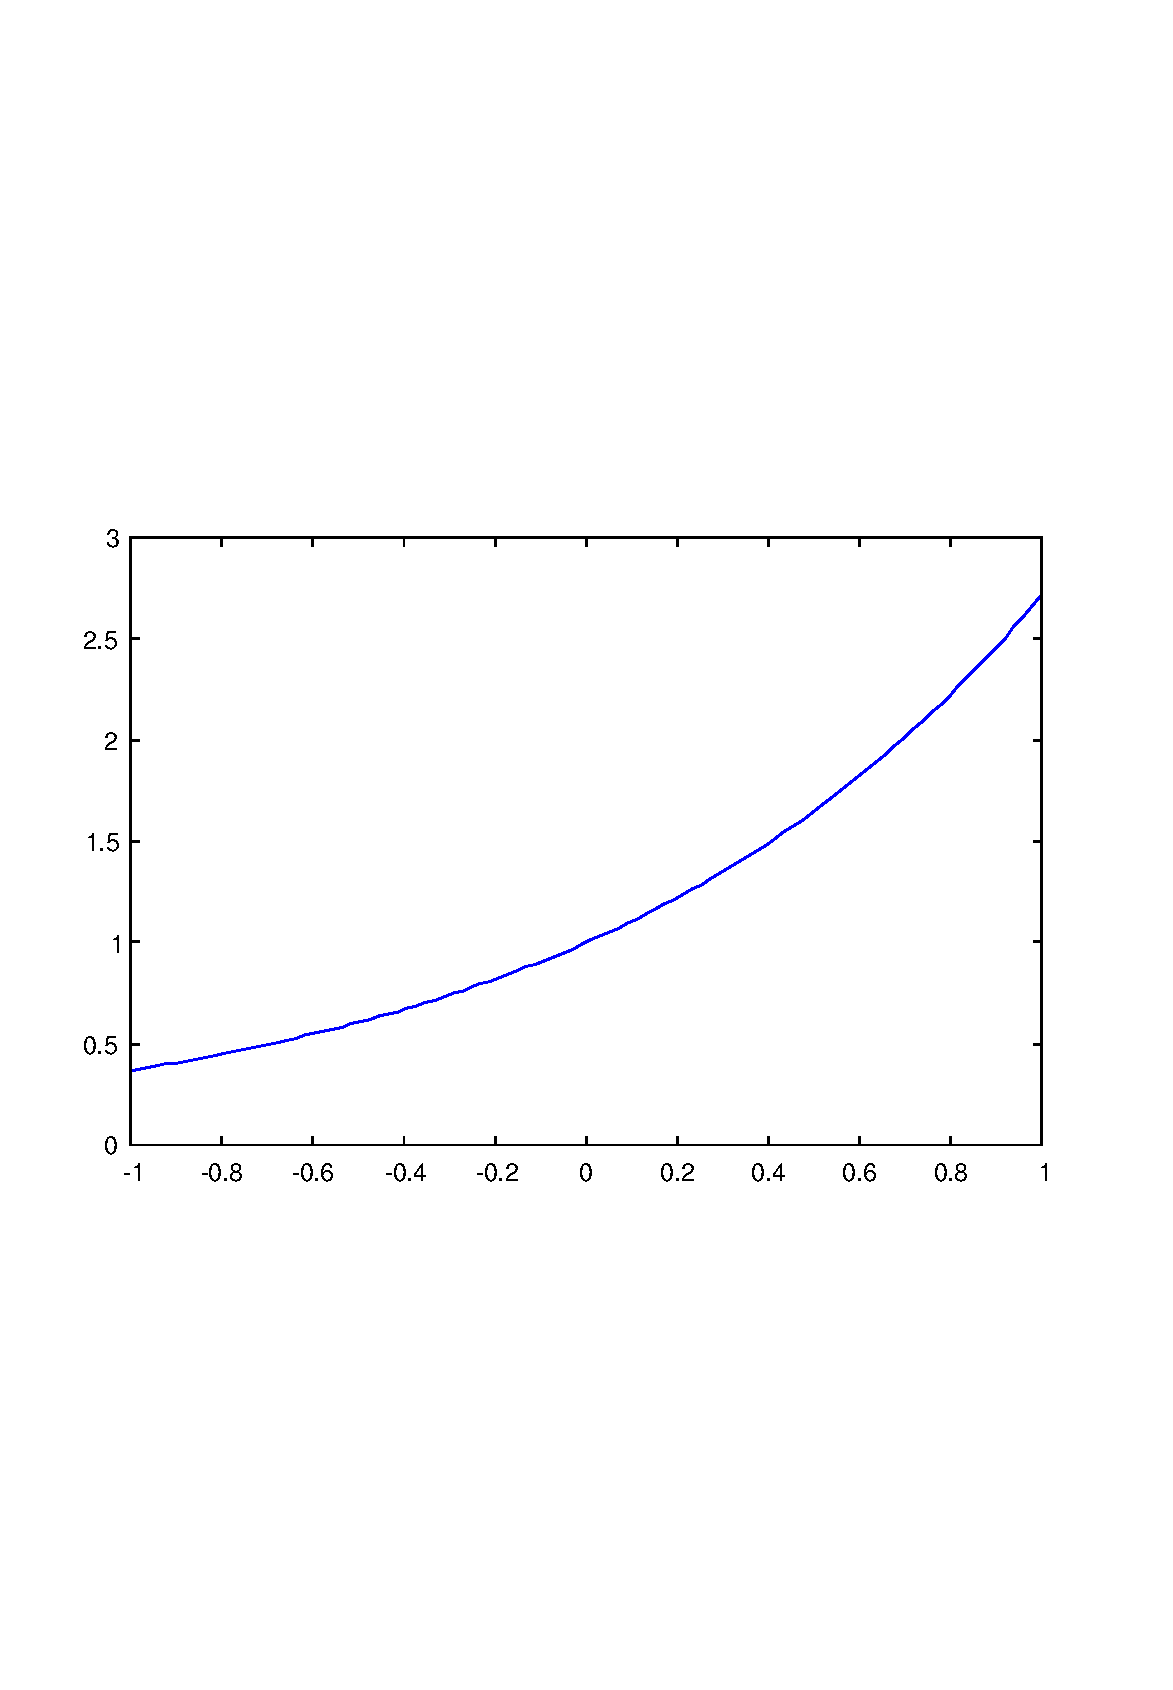
\includegraphics[width=12cm]{expplot1}
\caption{expplot1}
\end{DoxyImage}
 In the second example, we plot the unit circle in the complex plane {\ttfamily e$^\wedge$\{i 2 pi x\}} for {\ttfamily x in \mbox{[}-\/1,1\mbox{]}}.


\begin{DoxyVerbInclude}
--> x = linspace(-1,1);
--> plot(exp(-i*x*2*pi))
\end{DoxyVerbInclude}


 
\begin{DoxyImage}
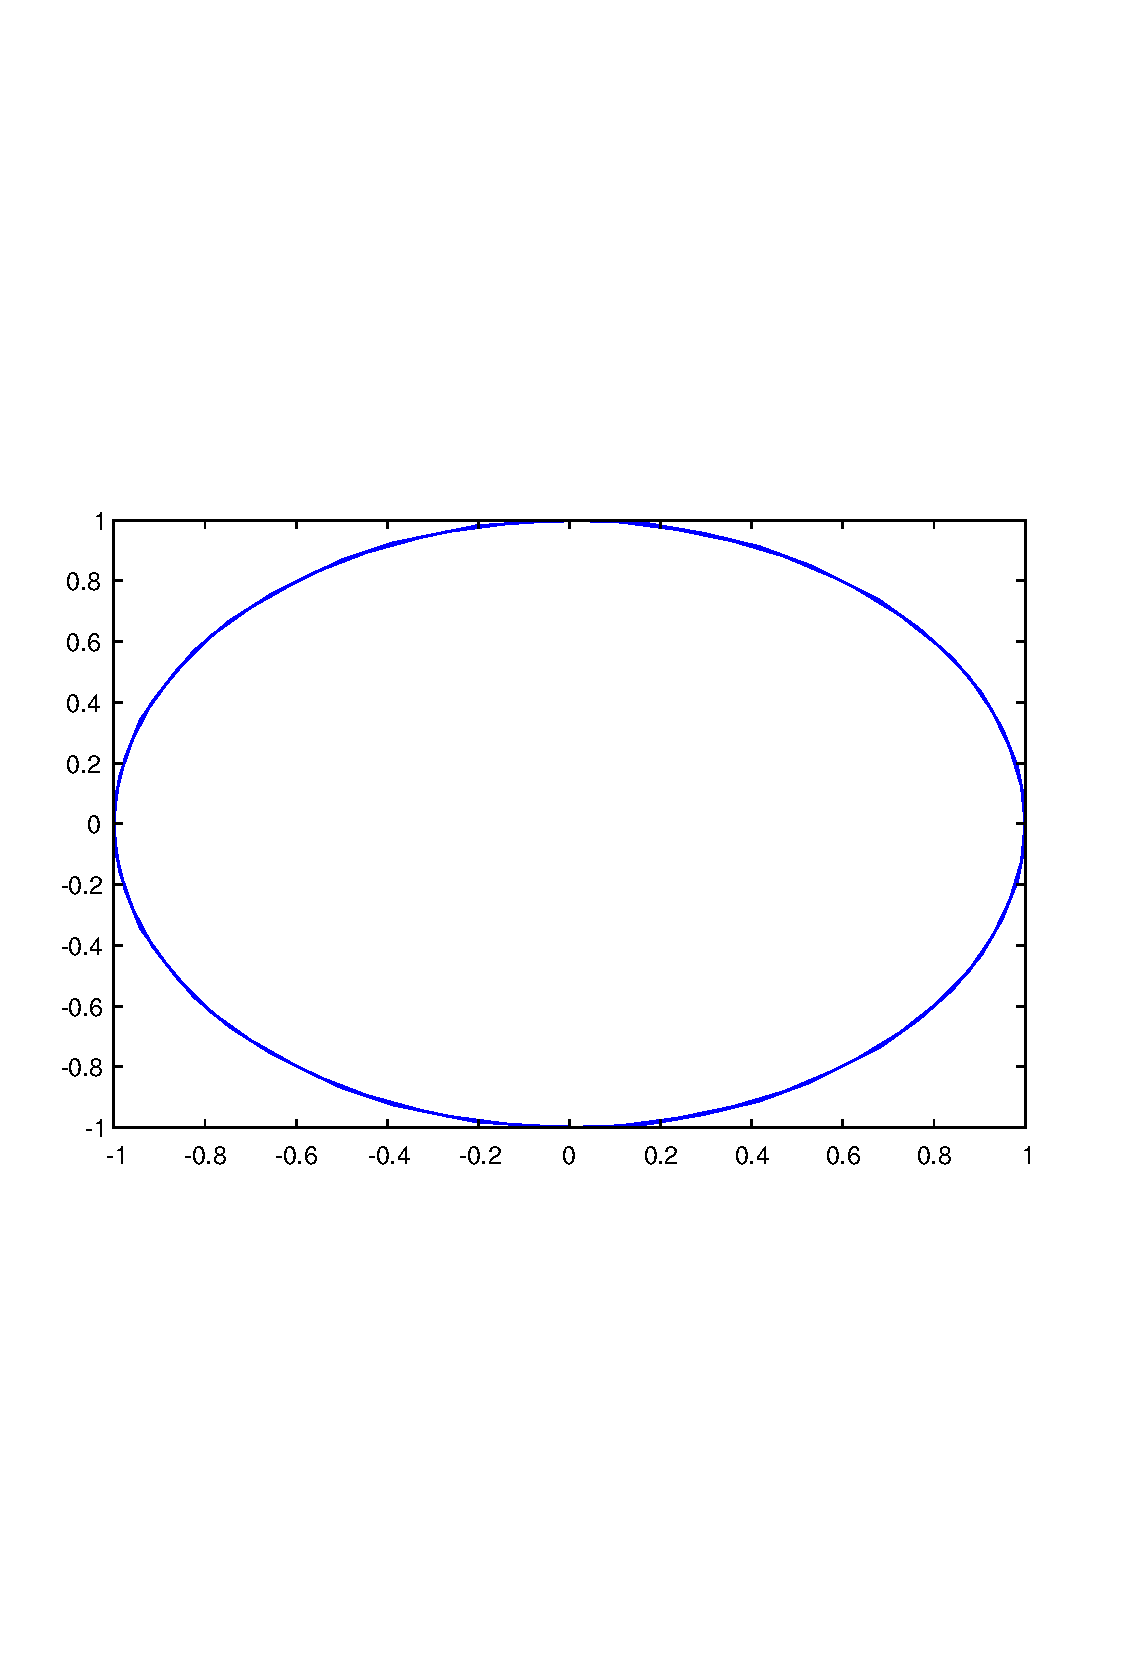
\includegraphics[width=12cm]{expplot2}
\caption{expplot2}
\end{DoxyImage}
 \hypertarget{mathfunctions_expm1}{}\section{E\-X\-P\-M1 Exponential Minus One Function}\label{mathfunctions_expm1}
Section\-: \hyperlink{sec_mathfunctions}{Mathematical Functions} \hypertarget{vtkwidgets_vtkxyplotwidget_Usage}{}\subsection{Usage}\label{vtkwidgets_vtkxyplotwidget_Usage}
Computes {\ttfamily exp(x)-\/1} function accurately for {\ttfamily x} small. The syntax for its use is \begin{DoxyVerb}   y = expm1(x)
\end{DoxyVerb}
 where {\ttfamily x} is an {\ttfamily n}-\/dimensional array of numerical type. \hypertarget{mathfunctions_fix}{}\section{F\-I\-X Round Towards Zero}\label{mathfunctions_fix}
Section\-: \hyperlink{sec_mathfunctions}{Mathematical Functions} \hypertarget{vtkwidgets_vtkxyplotwidget_Usage}{}\subsection{Usage}\label{vtkwidgets_vtkxyplotwidget_Usage}
Rounds the argument array towards zero. The syntax for its use is \begin{DoxyVerb}   y = fix(x)
\end{DoxyVerb}
 where {\ttfamily x} is a numeric array. For positive elements of {\ttfamily x}, the output is the largest integer smaller than {\ttfamily x}. For negative elements of {\ttfamily x} the output is the smallest integer larger than {\ttfamily x}. For complex {\ttfamily x}, the operation is applied seperately to the real and imaginary parts. \hypertarget{variables_struct_Example}{}\subsection{Example}\label{variables_struct_Example}
Here is a simple example of the {\ttfamily fix} operation on some values


\begin{DoxyVerbInclude}
--> a = [-1.8,pi,8,-pi,-0.001,2.3+0.3i]

a = 

 Columns 1 to 3

  -1.8000 +  0.0000i   3.1416 +  0.0000i   8.0000 +  0.0000i 

 Columns 4 to 6

  -3.1416 +  0.0000i  -0.0010 +  0.0000i   2.3000 +  0.3000i 

--> fix(a)

ans = 

 Columns 1 to 3

  -1.0000 +  0.0000i   3.0000 +  0.0000i   8.0000 +  0.0000i 

 Columns 4 to 6

  -3.0000 +  0.0000i        0             2.0000 +  0.0000i 
\end{DoxyVerbInclude}
 \hypertarget{mathfunctions_gamma}{}\section{G\-A\-M\-M\-A Gamma Function}\label{mathfunctions_gamma}
Section\-: \hyperlink{sec_mathfunctions}{Mathematical Functions} \hypertarget{vtkwidgets_vtkxyplotwidget_Usage}{}\subsection{Usage}\label{vtkwidgets_vtkxyplotwidget_Usage}
Computes the gamma function for real arguments. The {\ttfamily gamma} function takes only a single argument \begin{DoxyVerb}  y = gamma(x)
\end{DoxyVerb}
 where {\ttfamily x} is either a {\ttfamily float} or {\ttfamily double} array. The output vector {\ttfamily y} is the same size (and type) as {\ttfamily x}. \hypertarget{transforms_svd_Function}{}\subsection{Internals}\label{transforms_svd_Function}
The gamma function is defined by the integral\-: \[ \Gamma(x) = \int_{0}^{\infty} e^{-t} t^{x-1} \, dt \] The gamma function obeys the interesting relationship \[ \Gamma(x) = (x-1)\Gamma(x-1), \] and for integer arguments, is equivalent to the factorial function. \hypertarget{variables_struct_Example}{}\subsection{Example}\label{variables_struct_Example}
Here is a plot of the gamma function over the range {\ttfamily \mbox{[}-\/5,5\mbox{]}}.


\begin{DoxyVerbInclude}
--> x = linspace(-5,5);
--> y = gamma(x);
--> plot(x,y); xlabel('x'); ylabel('gamma(x)');
--> axis([-5,5,-5,5]);
\end{DoxyVerbInclude}


which results in the following plot.  
\begin{DoxyImage}
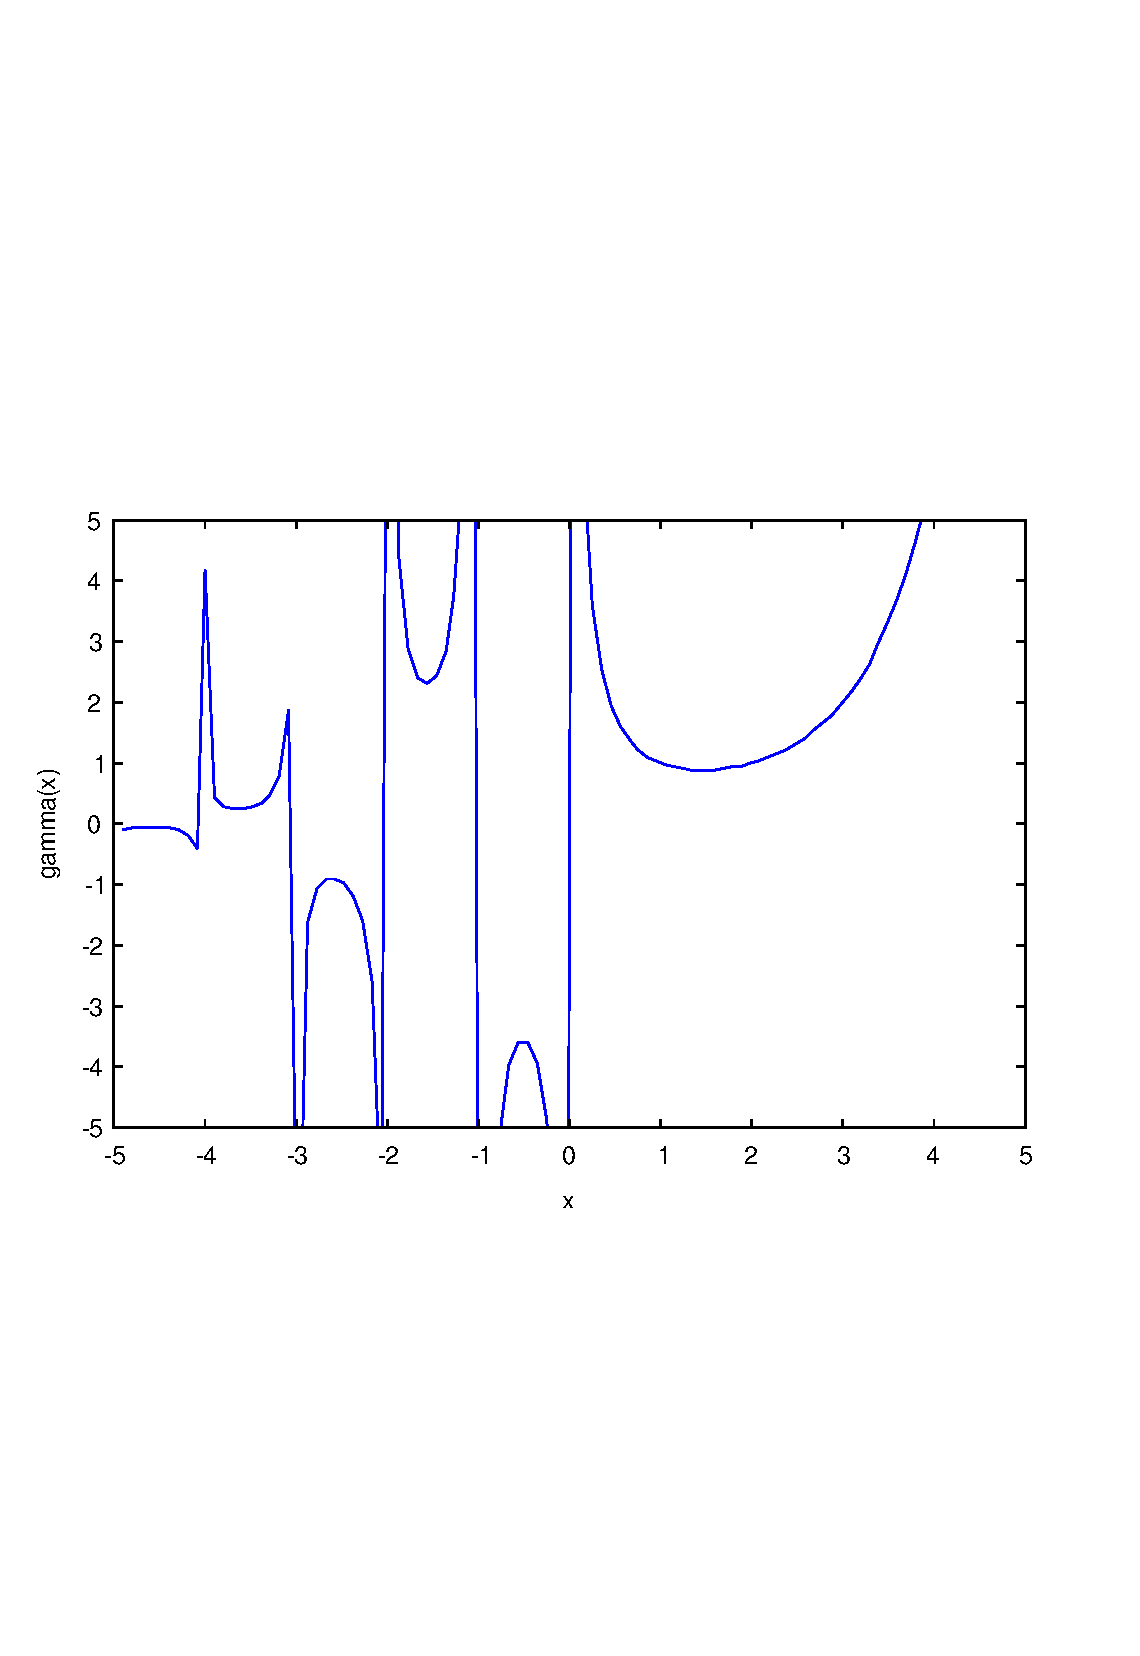
\includegraphics[width=12cm]{gamma1}
\caption{gamma1}
\end{DoxyImage}
 \hypertarget{mathfunctions_gammaln}{}\section{G\-A\-M\-M\-A\-L\-N Log Gamma Function}\label{mathfunctions_gammaln}
Section\-: \hyperlink{sec_mathfunctions}{Mathematical Functions} \hypertarget{vtkwidgets_vtkxyplotwidget_Usage}{}\subsection{Usage}\label{vtkwidgets_vtkxyplotwidget_Usage}
Computes the natural log of the gamma function for real arguments. The {\ttfamily gammaln} function takes only a single argument \begin{DoxyVerb}  y = gammaln(x)
\end{DoxyVerb}
 where {\ttfamily x} is either a {\ttfamily float} or {\ttfamily double} array. The output vector {\ttfamily y} is the same size (and type) as {\ttfamily x}. \hypertarget{variables_struct_Example}{}\subsection{Example}\label{variables_struct_Example}
Here is a plot of the {\ttfamily gammaln} function over the range {\ttfamily \mbox{[}-\/5,5\mbox{]}}.


\begin{DoxyVerbInclude}
--> x = linspace(0,10);
--> y = gammaln(x);
--> plot(x,y); xlabel('x'); ylabel('gammaln(x)');
\end{DoxyVerbInclude}


which results in the following plot.  
\begin{DoxyImage}
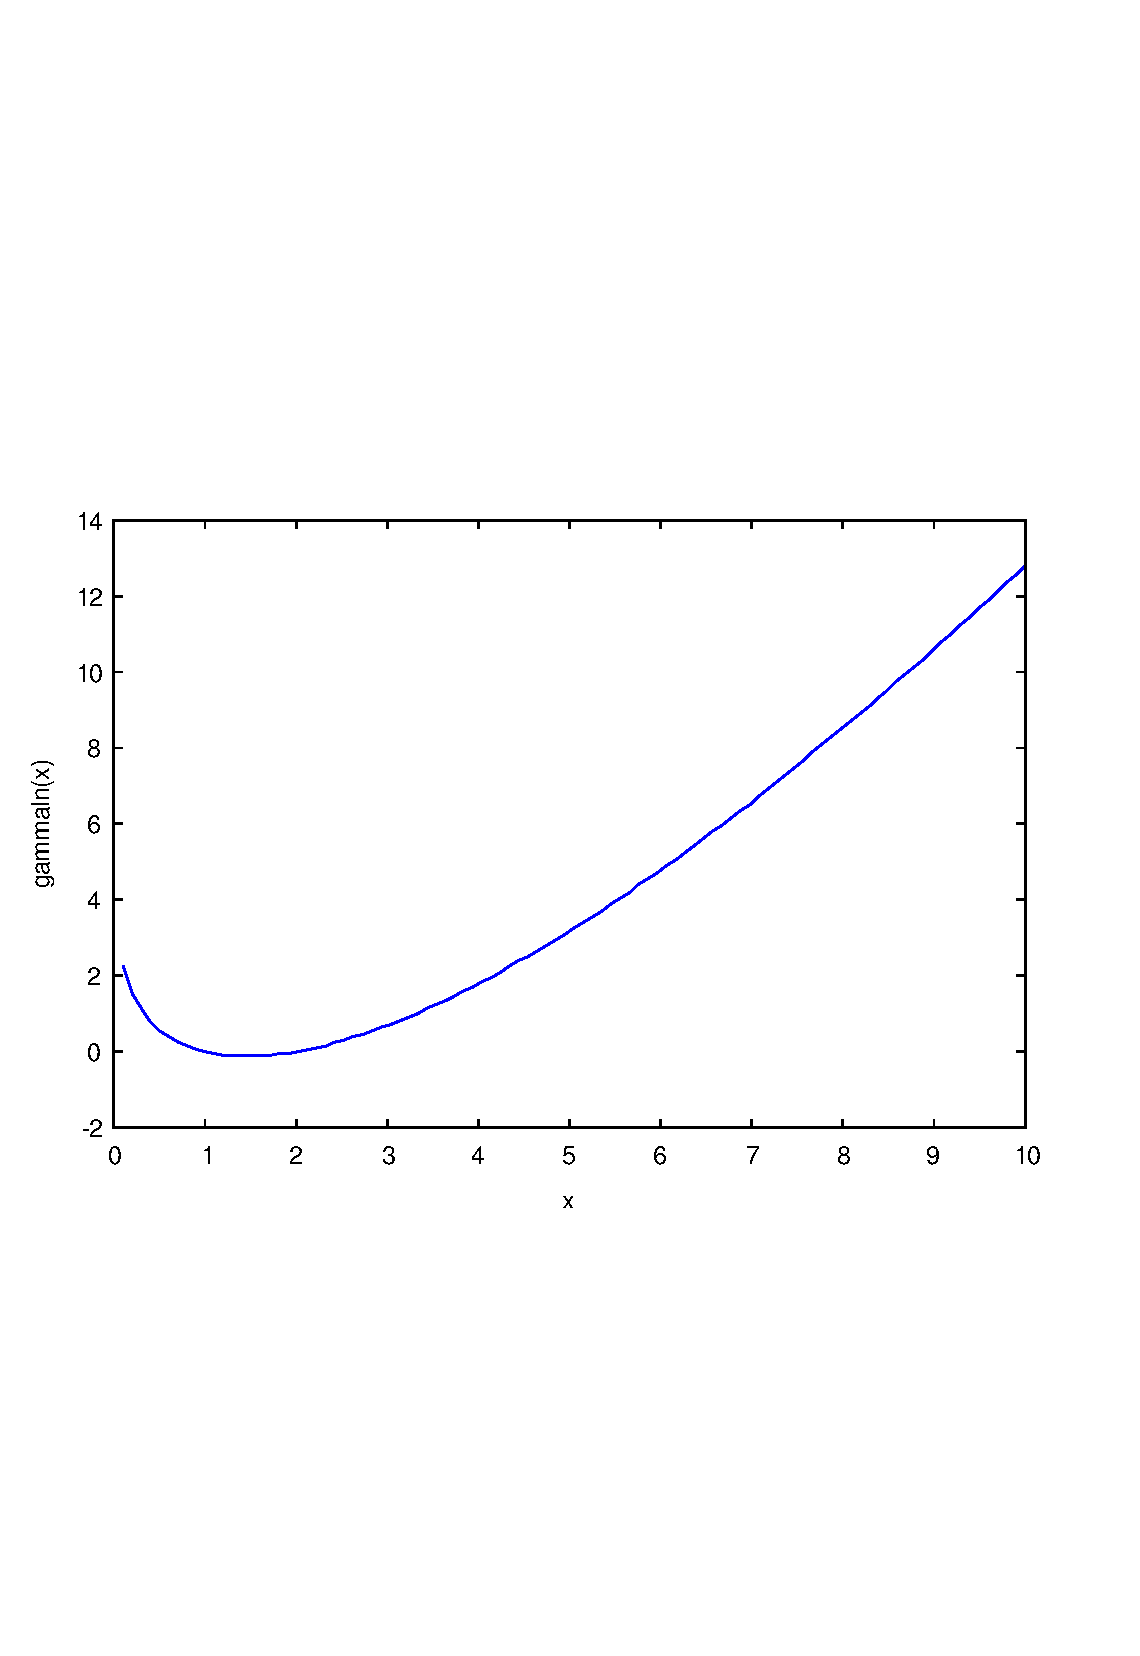
\includegraphics[width=12cm]{gammaln1}
\caption{gammaln1}
\end{DoxyImage}
 \hypertarget{mathfunctions_idiv}{}\section{I\-D\-I\-V Integer Division Operation}\label{mathfunctions_idiv}
Section\-: \hyperlink{sec_mathfunctions}{Mathematical Functions} \hypertarget{vtkwidgets_vtkxyplotwidget_Usage}{}\subsection{Usage}\label{vtkwidgets_vtkxyplotwidget_Usage}
Computes the integer division of two arrays. The syntax for its use is \begin{DoxyVerb}   y = idiv(a,b)
\end{DoxyVerb}
 where {\ttfamily a} and {\ttfamily b} are arrays or scalars. The effect of the {\ttfamily idiv} is to compute the integer division of {\ttfamily b} into {\ttfamily a}. \hypertarget{variables_struct_Example}{}\subsection{Example}\label{variables_struct_Example}
The following examples show some uses of {\ttfamily idiv} arrays.


\begin{DoxyVerbInclude}
--> idiv(27,6)

ans = 
 4 

--> idiv(4,-2)

ans = 
 -2 

--> idiv(15,3)

ans = 
 5 
\end{DoxyVerbInclude}
 \hypertarget{mathfunctions_legendre}{}\section{L\-E\-G\-E\-N\-D\-R\-E Associated Legendre Polynomial}\label{mathfunctions_legendre}
Section\-: \hyperlink{sec_mathfunctions}{Mathematical Functions} \hypertarget{vtkwidgets_vtkxyplotwidget_Usage}{}\subsection{Usage}\label{vtkwidgets_vtkxyplotwidget_Usage}
Computes the associated Legendre function of degree n. \begin{DoxyVerb}  y = legendre(n,x)
\end{DoxyVerb}
 where {\ttfamily x} is either a {\ttfamily float} or {\ttfamily double} array in range {\ttfamily \mbox{[}-\/1,1\mbox{]}}, {\ttfamily n} is integer scalar. The output vector {\ttfamily y} is the same size (and type) as {\ttfamily x}. \hypertarget{variables_struct_Example}{}\subsection{Example}\label{variables_struct_Example}
Here is a plot of the {\ttfamily legendre} function over the range {\ttfamily \mbox{[}-\/1,1\mbox{]}}.


\begin{DoxyVerbInclude}
--> x = linspace(-1,1,30);
--> y = legendre(4,x);
--> plot(x,y); xlabel('x'); ylabel('legendre(4,x)');
\end{DoxyVerbInclude}


which results in the following plot.  
\begin{DoxyImage}
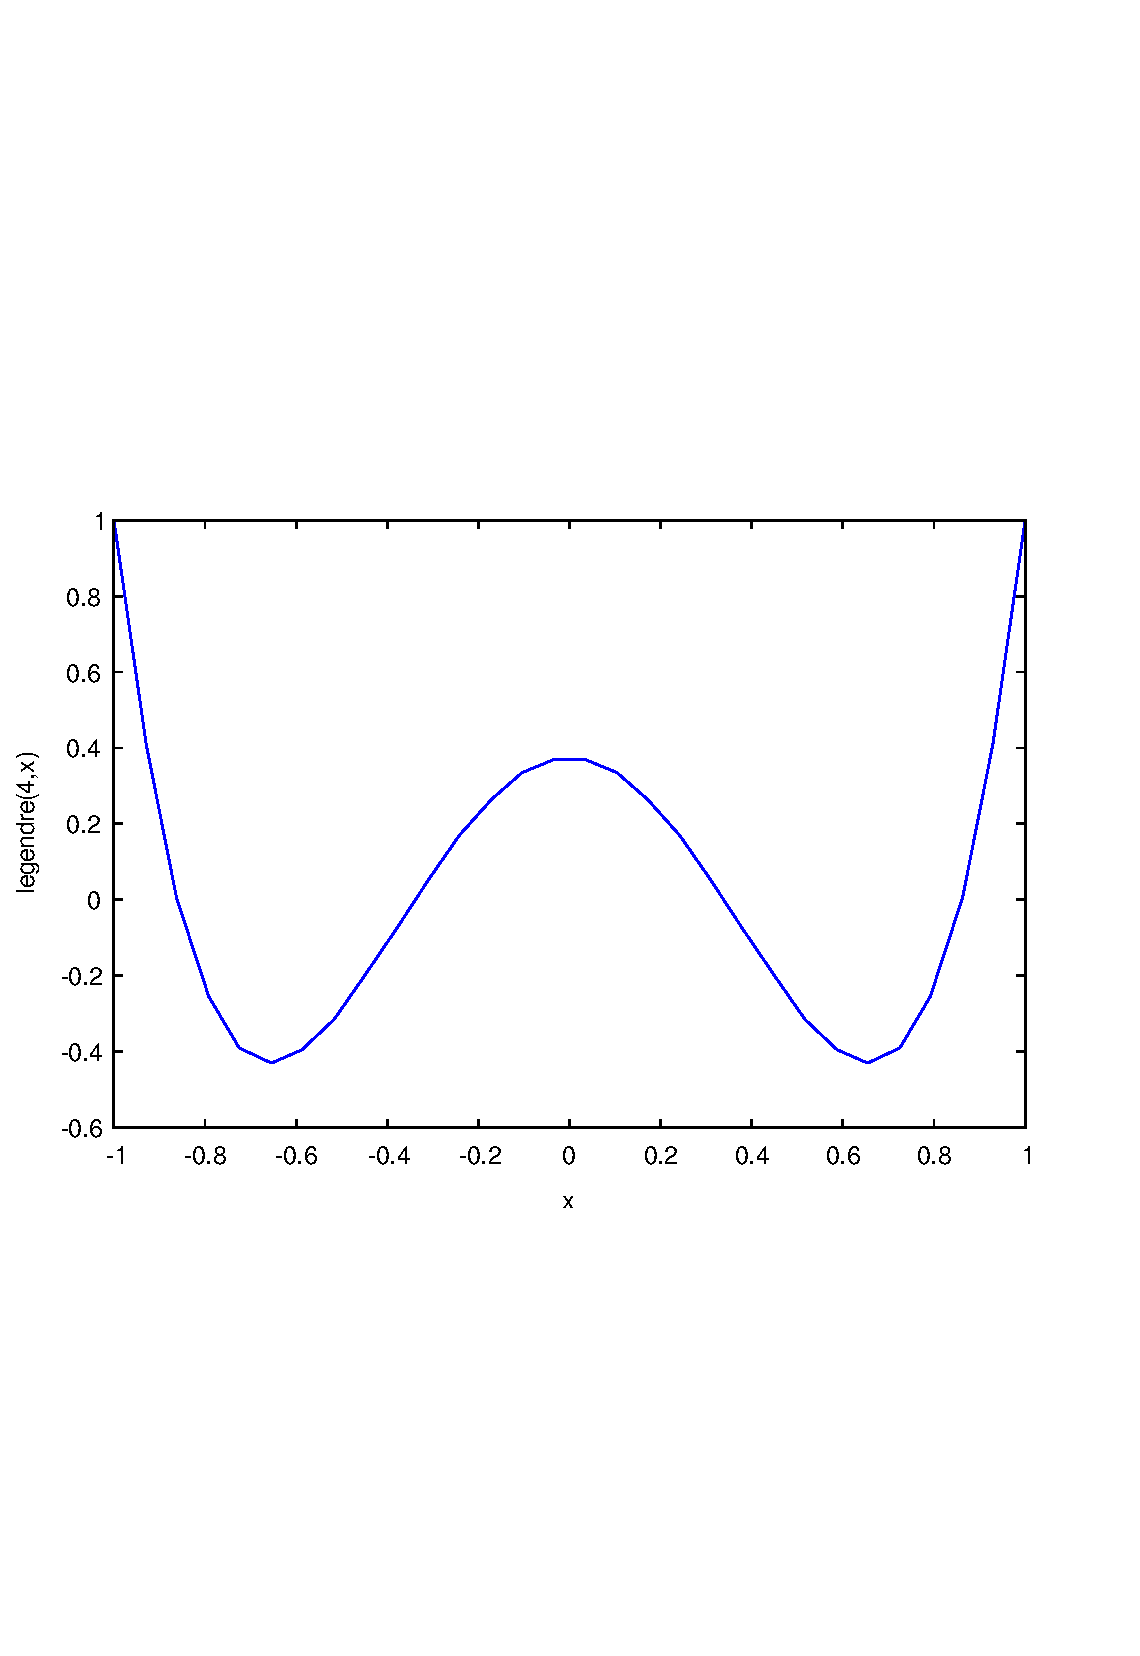
\includegraphics[width=12cm]{legendre}
\caption{legendre}
\end{DoxyImage}
 \hypertarget{mathfunctions_log}{}\section{L\-O\-G Natural Logarithm Function}\label{mathfunctions_log}
Section\-: \hyperlink{sec_mathfunctions}{Mathematical Functions} \hypertarget{vtkwidgets_vtkxyplotwidget_Usage}{}\subsection{Usage}\label{vtkwidgets_vtkxyplotwidget_Usage}
Computes the {\ttfamily log} function for its argument. The general syntax for its use is \begin{DoxyVerb}  y = log(x)
\end{DoxyVerb}
 where {\ttfamily x} is an {\ttfamily n}-\/dimensional array of numerical type. Integer types are promoted to the {\ttfamily double} type prior to calculation of the {\ttfamily log} function. Output {\ttfamily y} is of the same size as the input {\ttfamily x}. For strictly positive, real inputs, the output type is the same as the input. For negative and complex arguments, the output is complex. \hypertarget{transforms_svd_Function}{}\subsection{Internals}\label{transforms_svd_Function}
Mathematically, the {\ttfamily log} function is defined for all real valued arguments {\ttfamily x} by the integral \[ \log x \equiv \int_1^{x} \frac{d\,t}{t}. \] For complex-\/valued arguments, {\ttfamily z}, the complex logarithm is defined as \[ \log z \equiv \log |z| + i \arg z, \] where {\ttfamily arg} is the complex argument of {\ttfamily z}. \hypertarget{variables_struct_Example}{}\subsection{Example}\label{variables_struct_Example}
The following piece of code plots the real-\/valued {\ttfamily log} function over the interval {\ttfamily \mbox{[}1,100\mbox{]}}\-:


\begin{DoxyVerbInclude}
--> x = linspace(1,100);
--> plot(x,log(x))
--> xlabel('x');
--> ylabel('log(x)');
\end{DoxyVerbInclude}


 
\begin{DoxyImage}
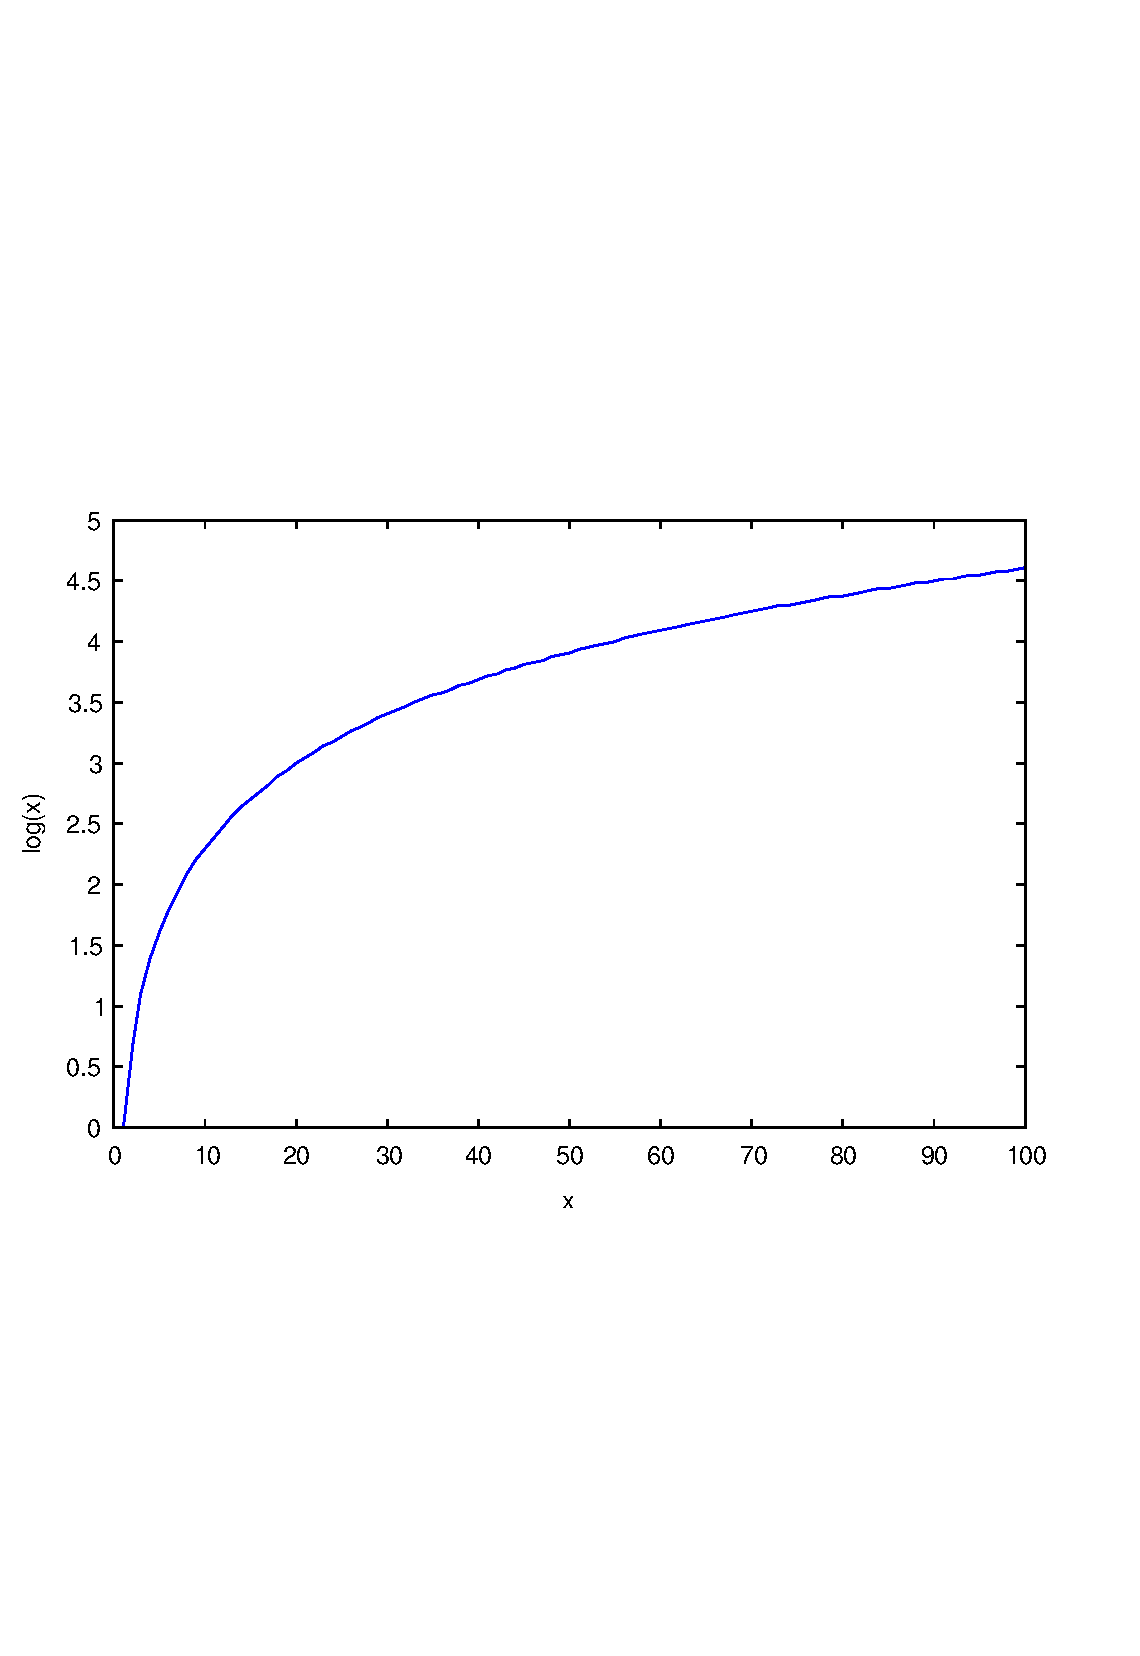
\includegraphics[width=12cm]{logplot}
\caption{logplot}
\end{DoxyImage}
 \hypertarget{mathfunctions_log10}{}\section{L\-O\-G10 Base-\/10 Logarithm Function}\label{mathfunctions_log10}
Section\-: \hyperlink{sec_mathfunctions}{Mathematical Functions} \hypertarget{vtkwidgets_vtkxyplotwidget_Usage}{}\subsection{Usage}\label{vtkwidgets_vtkxyplotwidget_Usage}
Computes the {\ttfamily log10} function for its argument. The general syntax for its use is \begin{DoxyVerb}  y = log10(x)
\end{DoxyVerb}
 where {\ttfamily x} is an {\ttfamily n}-\/dimensional array of numerical type. Integer types are promoted to the {\ttfamily double} type prior to calculation of the {\ttfamily log10} function. Output {\ttfamily y} is of the same size as the input {\ttfamily x}. For strictly positive, real inputs, the output type is the same as the input. For negative and complex arguments, the output is complex. \hypertarget{variables_struct_Example}{}\subsection{Example}\label{variables_struct_Example}
The following piece of code plots the real-\/valued {\ttfamily log10} function over the interval {\ttfamily \mbox{[}1,100\mbox{]}}\-:


\begin{DoxyVerbInclude}
--> x = linspace(1,100);
--> plot(x,log10(x))
--> xlabel('x');
--> ylabel('log10(x)');
\end{DoxyVerbInclude}


 
\begin{DoxyImage}
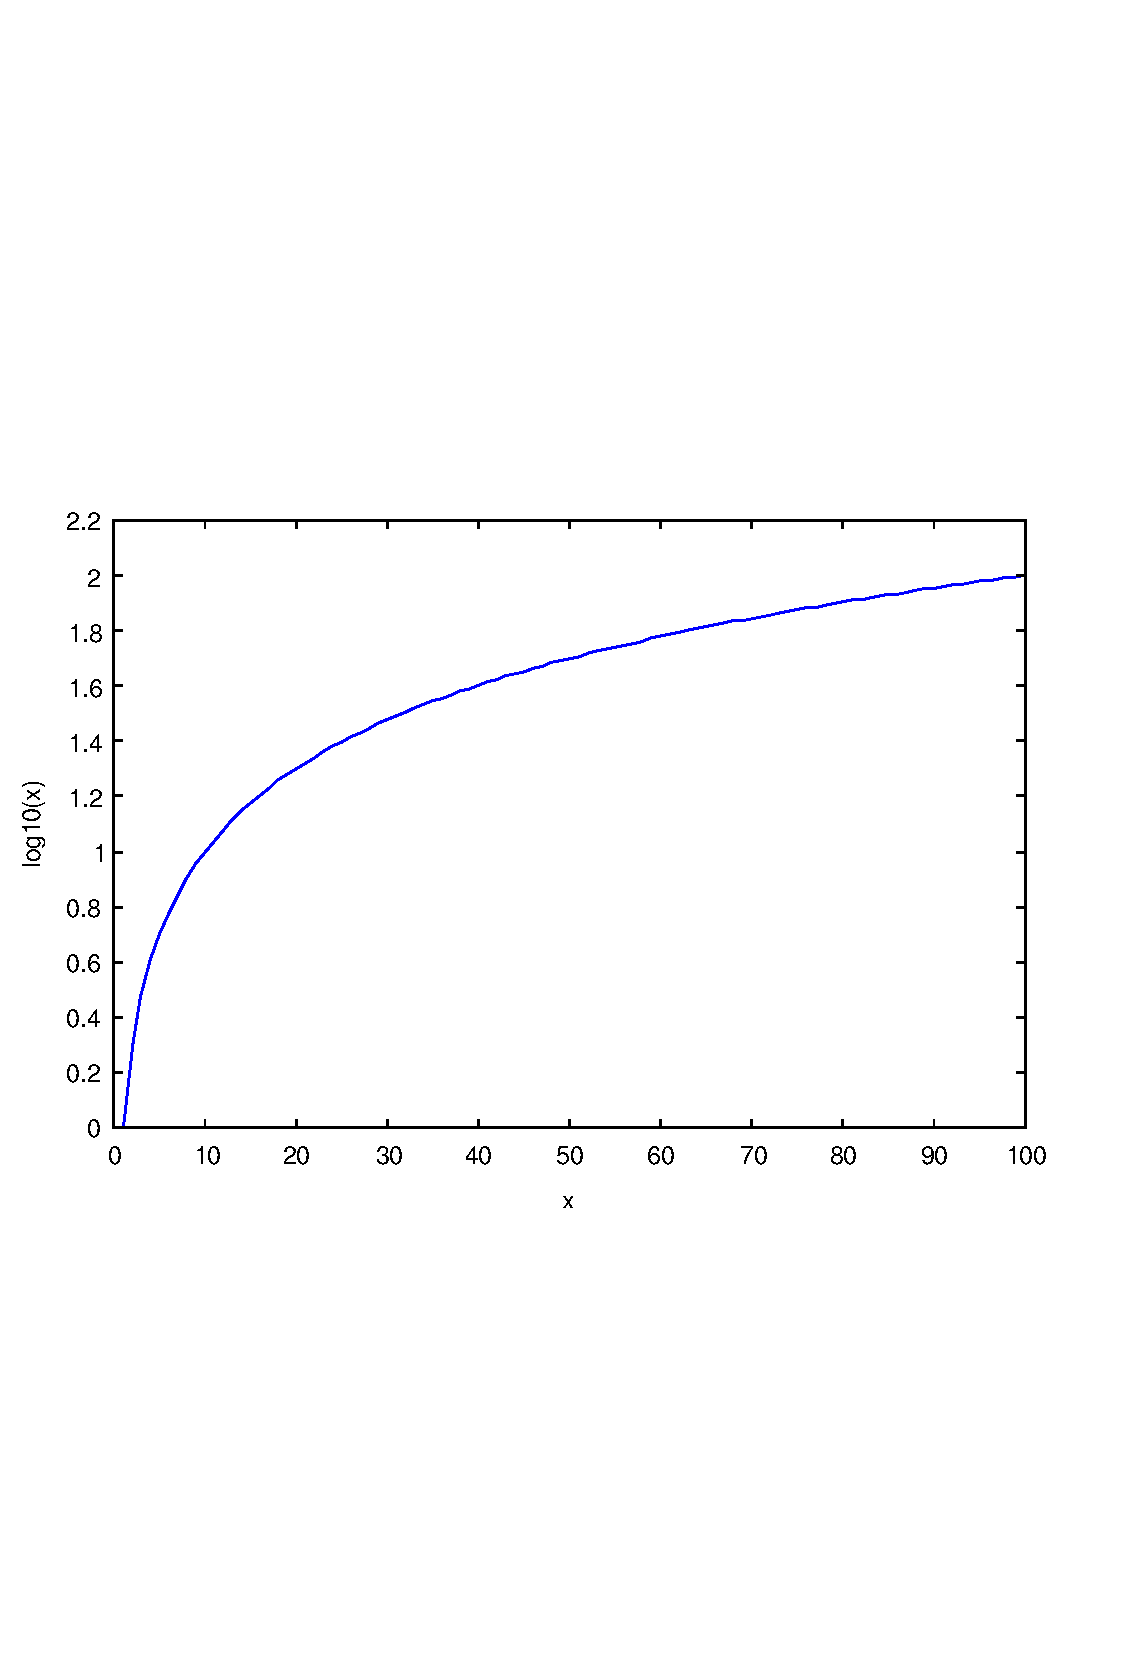
\includegraphics[width=12cm]{log10plot}
\caption{log10plot}
\end{DoxyImage}
 \hypertarget{mathfunctions_log1p}{}\section{L\-O\-G1\-P Natural Logarithm of 1+\-P Function}\label{mathfunctions_log1p}
Section\-: \hyperlink{sec_mathfunctions}{Mathematical Functions} \hypertarget{vtkwidgets_vtkxyplotwidget_Usage}{}\subsection{Usage}\label{vtkwidgets_vtkxyplotwidget_Usage}
Computes the {\ttfamily log} function for one plus its argument. The general syntax for its use is \begin{DoxyVerb}  y = log1p(x)
\end{DoxyVerb}
 where {\ttfamily x} is an {\ttfamily n}-\/dimensional array of numerical type. \hypertarget{mathfunctions_log2}{}\section{L\-O\-G2 Base-\/2 Logarithm Function}\label{mathfunctions_log2}
Section\-: \hyperlink{sec_mathfunctions}{Mathematical Functions} \hypertarget{vtkwidgets_vtkxyplotwidget_Usage}{}\subsection{Usage}\label{vtkwidgets_vtkxyplotwidget_Usage}
Computes the {\ttfamily log2} function for its argument. The general syntax for its use is \begin{DoxyVerb}  y = log2(x)
\end{DoxyVerb}
 where {\ttfamily x} is an {\ttfamily n}-\/dimensional array of numerical type. Integer types are promoted to the {\ttfamily double} type prior to calculation of the {\ttfamily log2} function. Output {\ttfamily y} is of the same size as the input {\ttfamily x}. For strictly positive, real inputs, the output type is the same as the input. For negative and complex arguments, the output is complex. \hypertarget{variables_struct_Example}{}\subsection{Example}\label{variables_struct_Example}
The following piece of code plots the real-\/valued {\ttfamily log2} function over the interval {\ttfamily \mbox{[}1,100\mbox{]}}\-:


\begin{DoxyVerbInclude}
--> x = linspace(1,100);
--> plot(x,log2(x))
--> xlabel('x');
--> ylabel('log2(x)');
\end{DoxyVerbInclude}


 
\begin{DoxyImage}
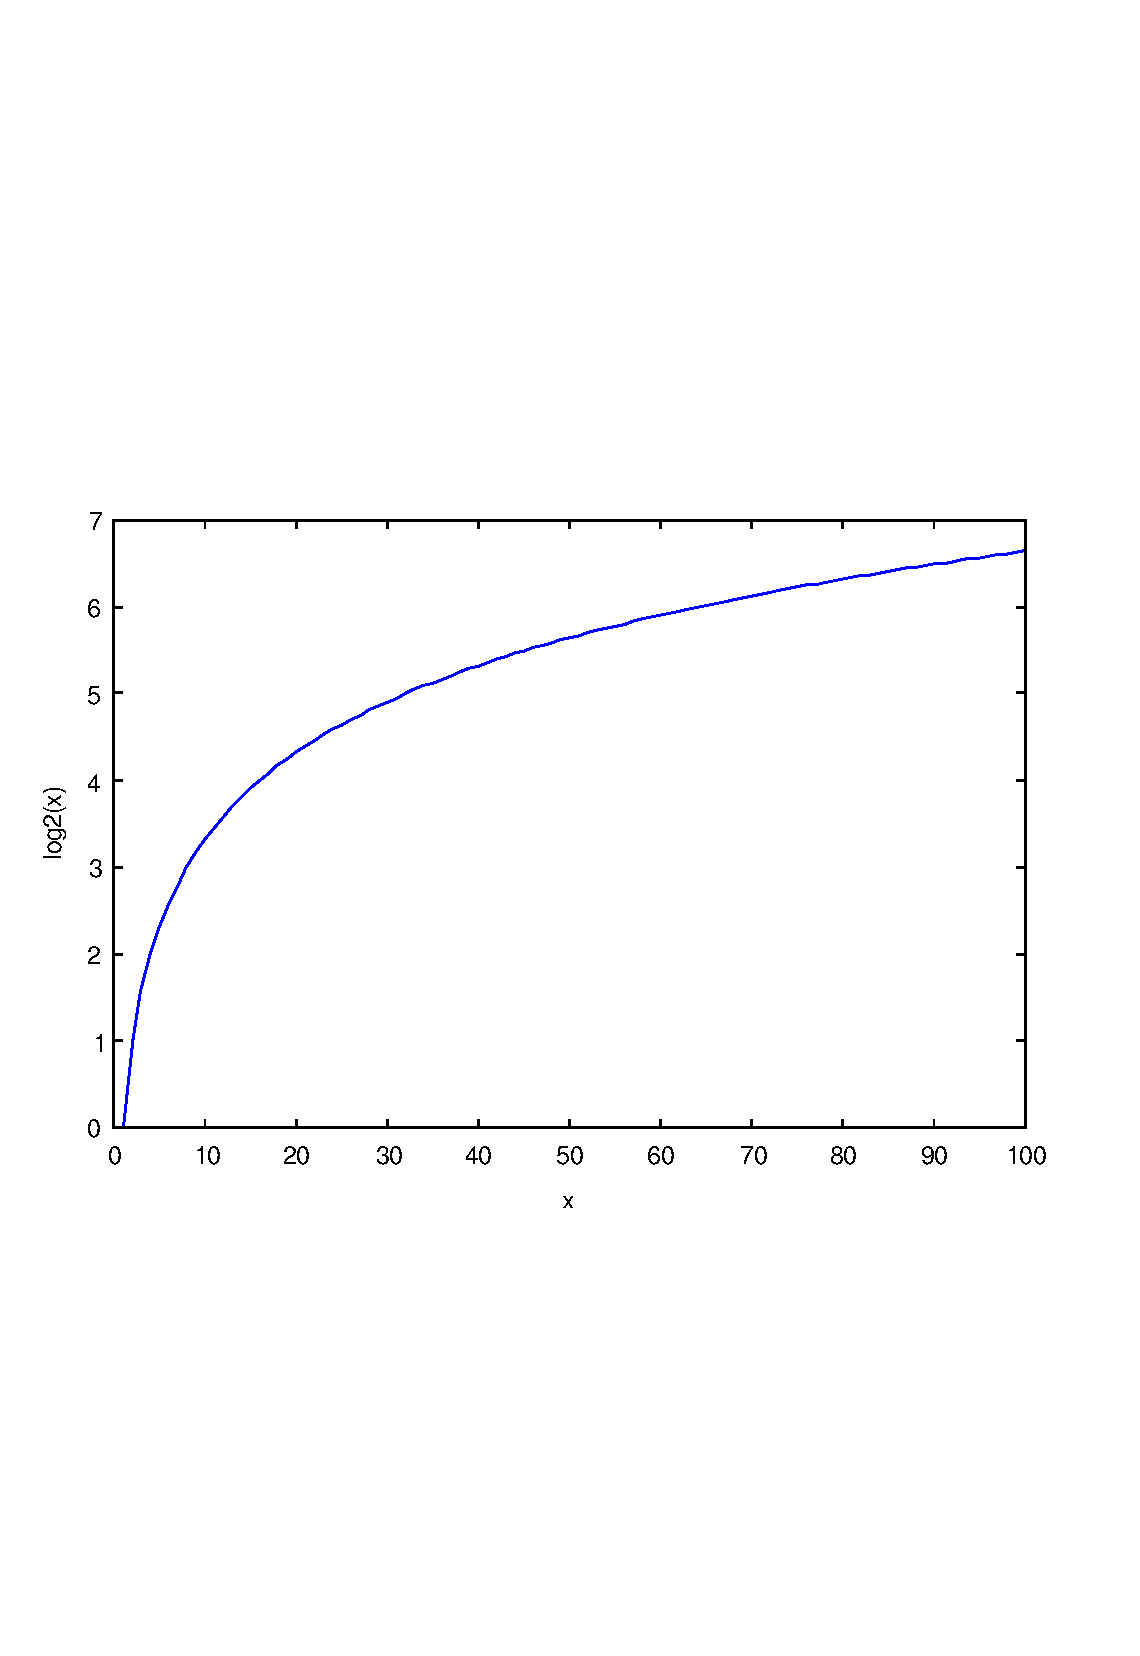
\includegraphics[width=12cm]{log2plot}
\caption{log2plot}
\end{DoxyImage}
 \hypertarget{mathfunctions_mod}{}\section{M\-O\-D Modulus Operation}\label{mathfunctions_mod}
Section\-: \hyperlink{sec_mathfunctions}{Mathematical Functions} \hypertarget{vtkwidgets_vtkxyplotwidget_Usage}{}\subsection{Usage}\label{vtkwidgets_vtkxyplotwidget_Usage}
Computes the modulus of an array. The syntax for its use is \begin{DoxyVerb}   y = mod(x,n)
\end{DoxyVerb}
 where {\ttfamily x} is matrix, and {\ttfamily n} is the base of the modulus. The effect of the {\ttfamily mod} operator is to add or subtract multiples of {\ttfamily n} to the vector {\ttfamily x} so that each element {\ttfamily x\-\_\-i} is between {\ttfamily 0} and {\ttfamily n} (strictly). Note that {\ttfamily n} does not have to be an integer. Also, {\ttfamily n} can either be a scalar (same base for all elements of {\ttfamily x}), or a vector (different base for each element of {\ttfamily x}).

Note that the following are defined behaviors\-: 
\begin{DoxyEnumerate}
\item {\ttfamily mod(x,0) = x}@  
\item {\ttfamily mod(x,x) = 0}@  
\item {\ttfamily mod(x,n)}@ has the same sign as {\ttfamily n} for all other cases.  
\end{DoxyEnumerate}\hypertarget{variables_struct_Example}{}\subsection{Example}\label{variables_struct_Example}
The following examples show some uses of {\ttfamily mod} arrays.


\begin{DoxyVerbInclude}
--> mod(18,12)

ans = 
 6 

--> mod(6,5)

ans = 
 1 

--> mod(2*pi,pi)

ans = 
 0 
\end{DoxyVerbInclude}


Here is an example of using {\ttfamily mod} to determine if integers are even or odd\-:


\begin{DoxyVerbInclude}
--> mod([1,3,5,2],2)

ans = 
 1 1 1 0 
\end{DoxyVerbInclude}


Here we use the second form of {\ttfamily mod}, with each element using a separate base.


\begin{DoxyVerbInclude}
--> mod([9 3 2 0],[1 0 2 2])

ans = 
 0 3 0 0 
\end{DoxyVerbInclude}
 \hypertarget{mathfunctions_mpower}{}\section{M\-P\-O\-W\-E\-R Matrix Power Function}\label{mathfunctions_mpower}
Section\-: \hyperlink{sec_mathfunctions}{Mathematical Functions} \hypertarget{vtkwidgets_vtkxyplotwidget_Usage}{}\subsection{Usage}\label{vtkwidgets_vtkxyplotwidget_Usage}
Computes the matrix power operator for two arrays. It is an M-\/file version of the {\ttfamily $^\wedge$} operator. The syntax for its use is \begin{DoxyVerb}   y = mpower(a,b)
\end{DoxyVerb}
 where {\ttfamily y=a$^\wedge$b}. See the {\ttfamily matrixpower} documentation for more details on what this function actually does. \hypertarget{mathfunctions_power}{}\section{P\-O\-W\-E\-R Element-\/wise Power Function}\label{mathfunctions_power}
Section\-: \hyperlink{sec_mathfunctions}{Mathematical Functions} \hypertarget{vtkwidgets_vtkxyplotwidget_Usage}{}\subsection{Usage}\label{vtkwidgets_vtkxyplotwidget_Usage}
Computes the element-\/wise power operator for two arrays. It is an M-\/file version of the {\ttfamily .$^\wedge$} operator. The syntax for its use is \begin{DoxyVerb}   y = power(a,b)
\end{DoxyVerb}
 where {\ttfamily y=a.$^\wedge$b}. See the {\ttfamily dotpower} documentation for more details on what this function actually does. \hypertarget{mathfunctions_rad2deg}{}\section{R\-A\-D2\-D\-E\-G Radians To Degrees Conversion Function}\label{mathfunctions_rad2deg}
Section\-: \hyperlink{sec_mathfunctions}{Mathematical Functions} \hypertarget{vtkwidgets_vtkxyplotwidget_Usage}{}\subsection{Usage}\label{vtkwidgets_vtkxyplotwidget_Usage}
Converts the argument array from radians to degrees. The general syntax for its use is \begin{DoxyVerb}   y = rad2deg(x)
\end{DoxyVerb}
 Note that the output type will be the same as the input type, and that complex arguments are allowed. The output is not wrapped to {\ttfamily \mbox{[}0,360)}. \hypertarget{variables_matrix_Examples}{}\subsection{Examples}\label{variables_matrix_Examples}
Some known conversion factors


\begin{DoxyVerbInclude}
--> rad2deg(1) % one radian is about 57 degrees

ans = 
   57.2958 

--> rad2deg(pi/4) % should be 45 degrees

ans = 
 45 

--> rad2deg(2*pi) % Note that this is 360 not 0 degrees

ans = 
 360 
\end{DoxyVerbInclude}
 \hypertarget{mathfunctions_rem}{}\section{R\-E\-M Remainder After Division}\label{mathfunctions_rem}
Section\-: \hyperlink{sec_mathfunctions}{Mathematical Functions} \hypertarget{vtkwidgets_vtkxyplotwidget_Usage}{}\subsection{Usage}\label{vtkwidgets_vtkxyplotwidget_Usage}
Computes the remainder after division of an array. The syntax for its use is \begin{DoxyVerb}   y = rem(x,n)
\end{DoxyVerb}
 where {\ttfamily x} is matrix, and {\ttfamily n} is the base of the modulus. The effect of the {\ttfamily rem} operator is to add or subtract multiples of {\ttfamily n} to the vector {\ttfamily x} so that each element {\ttfamily x\-\_\-i} is between {\ttfamily 0} and {\ttfamily n} (strictly). Note that {\ttfamily n} does not have to be an integer. Also, {\ttfamily n} can either be a scalar (same base for all elements of {\ttfamily x}), or a vector (different base for each element of {\ttfamily x}).

Note that the following are defined behaviors\-: 
\begin{DoxyEnumerate}
\item {\ttfamily rem(x,0) = nan}@  
\item {\ttfamily rem(x,x) = 0}@ for nonzero {\ttfamily x}  
\item {\ttfamily rem(x,n)}@ has the same sign as {\ttfamily x} for all other cases.  
\end{DoxyEnumerate}Note that {\ttfamily rem} and {\ttfamily mod} return the same value if {\ttfamily x} and {\ttfamily n} are of the same sign. But differ by {\ttfamily n} if {\ttfamily x} and {\ttfamily y} have different signs. \hypertarget{variables_struct_Example}{}\subsection{Example}\label{variables_struct_Example}
The following examples show some uses of {\ttfamily rem} arrays.


\begin{DoxyVerbInclude}
--> rem(18,12)

ans = 
 6 

--> rem(6,5)

ans = 
 1 

--> rem(2*pi,pi)

ans = 
 0 
\end{DoxyVerbInclude}


Here is an example of using {\ttfamily rem} to determine if integers are even or odd\-:


\begin{DoxyVerbInclude}
--> rem([1,3,5,2],2)

ans = 
 1 1 1 0 
\end{DoxyVerbInclude}


Here we use the second form of {\ttfamily rem}, with each element using a separate base.


\begin{DoxyVerbInclude}
--> rem([9 3 2 0],[1 0 2 2])

ans = 
         0 NaN         0         0 
\end{DoxyVerbInclude}
 \hypertarget{mathfunctions_sec}{}\section{S\-E\-C Trigonometric Secant Function}\label{mathfunctions_sec}
Section\-: \hyperlink{sec_mathfunctions}{Mathematical Functions} \hypertarget{vtkwidgets_vtkxyplotwidget_Usage}{}\subsection{Usage}\label{vtkwidgets_vtkxyplotwidget_Usage}
Computes the {\ttfamily sec} function for its argument. The general syntax for its use is \begin{DoxyVerb}  y = sec(x)
\end{DoxyVerb}
 where {\ttfamily x} is an {\ttfamily n}-\/dimensional array of numerical type. Integer types are promoted to the {\ttfamily double} type prior to calculation of the {\ttfamily sec} function. Output {\ttfamily y} is of the same size and type as the input {\ttfamily x}, (unless {\ttfamily x} is an integer, in which case {\ttfamily y} is a {\ttfamily double} type). \hypertarget{transforms_svd_Function}{}\subsection{Internals}\label{transforms_svd_Function}
Mathematically, the {\ttfamily sec} function is defined for all arguments as \[ \sec x \equiv \frac{1}{\cos x}. \] \hypertarget{variables_struct_Example}{}\subsection{Example}\label{variables_struct_Example}
The following piece of code plots the real-\/valued {\ttfamily sec(2 pi x)} function over the interval of {\ttfamily \mbox{[}-\/1,1\mbox{]}}\-:


\begin{DoxyVerbInclude}
--> t = linspace(-1,1,1000);
--> plot(t,sec(2*pi*t))
--> axis([-1,1,-10,10]);
\end{DoxyVerbInclude}


 
\begin{DoxyImage}
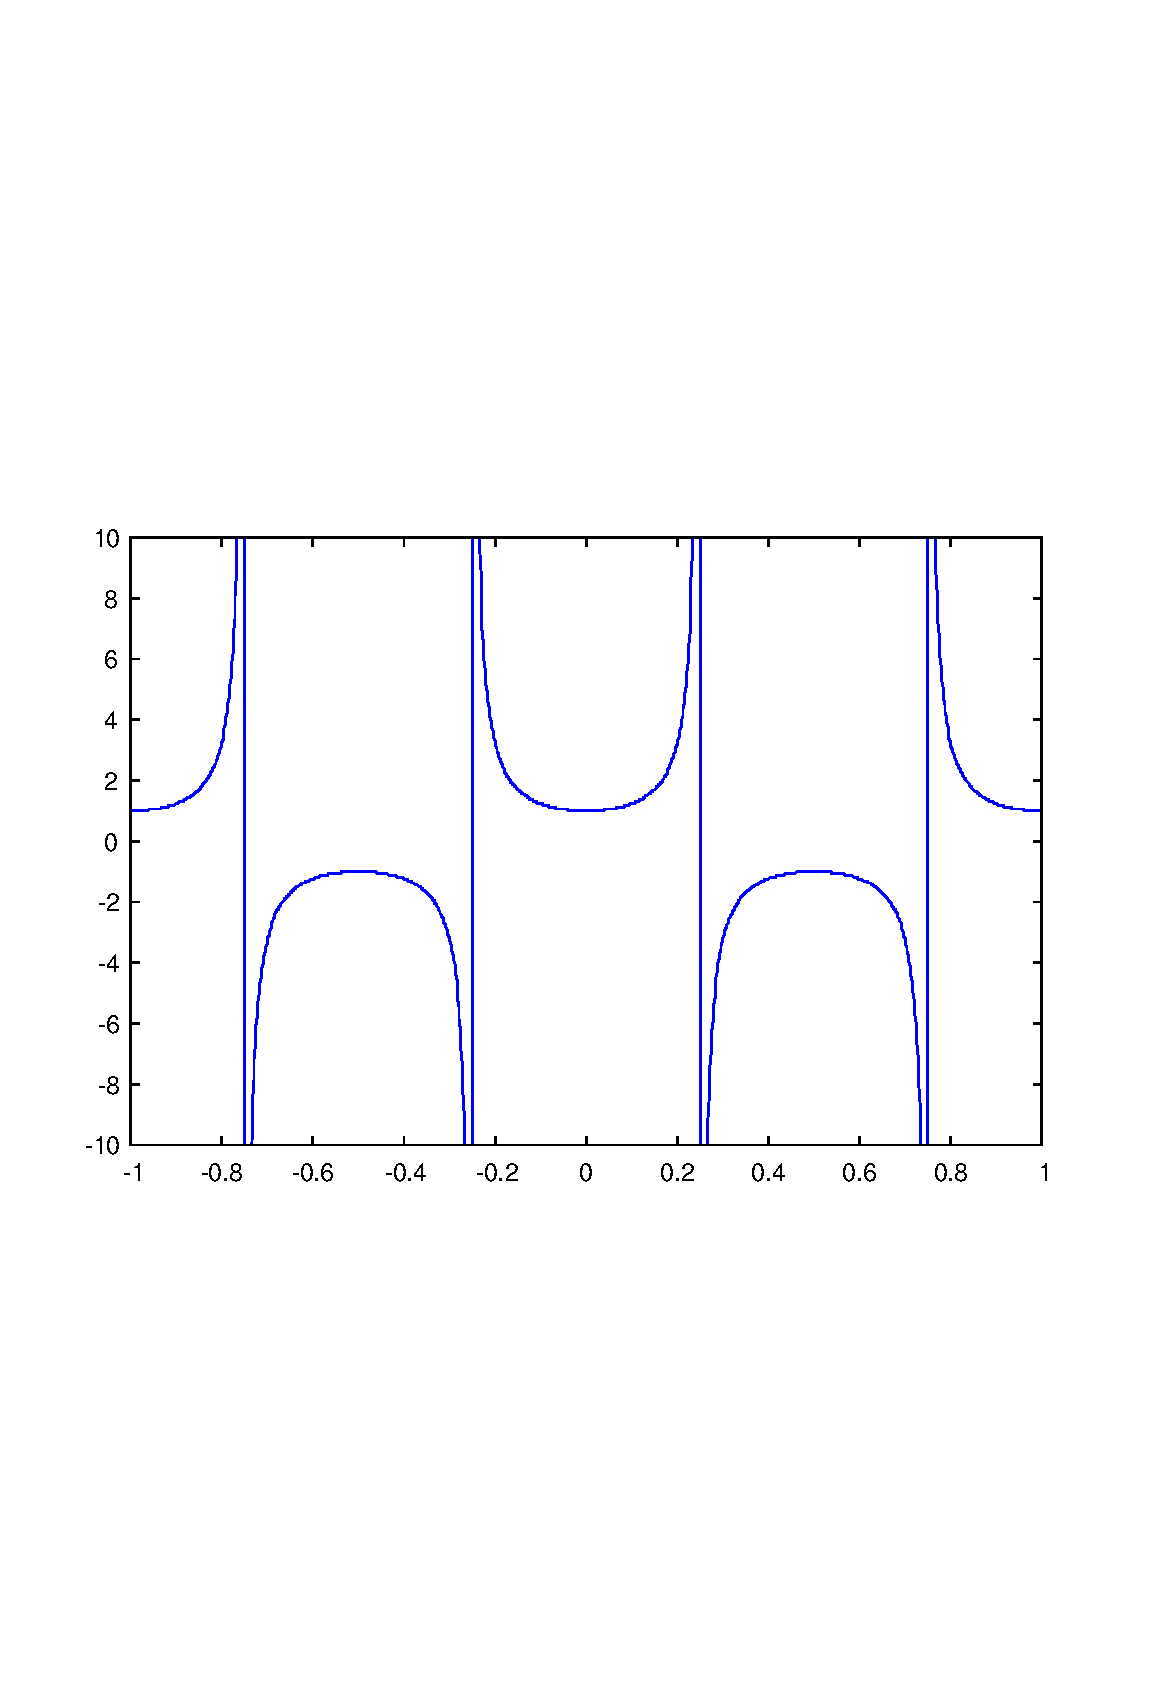
\includegraphics[width=12cm]{secplot}
\caption{secplot}
\end{DoxyImage}
 \hypertarget{mathfunctions_secd}{}\section{S\-E\-C\-D Secant Degrees Function}\label{mathfunctions_secd}
Section\-: \hyperlink{sec_mathfunctions}{Mathematical Functions} \hypertarget{vtkwidgets_vtkxyplotwidget_Usage}{}\subsection{Usage}\label{vtkwidgets_vtkxyplotwidget_Usage}
Computes the secant of the argument, but takes the argument in degrees instead of radians (as is the case for {\ttfamily sec}). The syntax for its use is \begin{DoxyVerb}   y = secd(x)
\end{DoxyVerb}
 \hypertarget{mathfunctions_sech}{}\section{S\-E\-C\-H Hyperbolic Secant Function}\label{mathfunctions_sech}
Section\-: \hyperlink{sec_mathfunctions}{Mathematical Functions} \hypertarget{vtkwidgets_vtkxyplotwidget_Usage}{}\subsection{Usage}\label{vtkwidgets_vtkxyplotwidget_Usage}
Computes the hyperbolic secant of the argument. The syntax for its use is \begin{DoxyVerb}   y = sech(x)
\end{DoxyVerb}
 \hypertarget{transforms_svd_Function}{}\subsection{Internals}\label{transforms_svd_Function}
The {\ttfamily sech} function is computed from the formula \[ \mathrm{sech}(x) = \frac{1}{\cosh(x)} \] \hypertarget{variables_matrix_Examples}{}\subsection{Examples}\label{variables_matrix_Examples}
Here is a simple plot of the hyperbolic secant function


\begin{DoxyVerbInclude}
--> x = -2*pi:.01:2*pi;
--> plot(x,sech(x)); grid('on');
\end{DoxyVerbInclude}


 
\begin{DoxyImage}
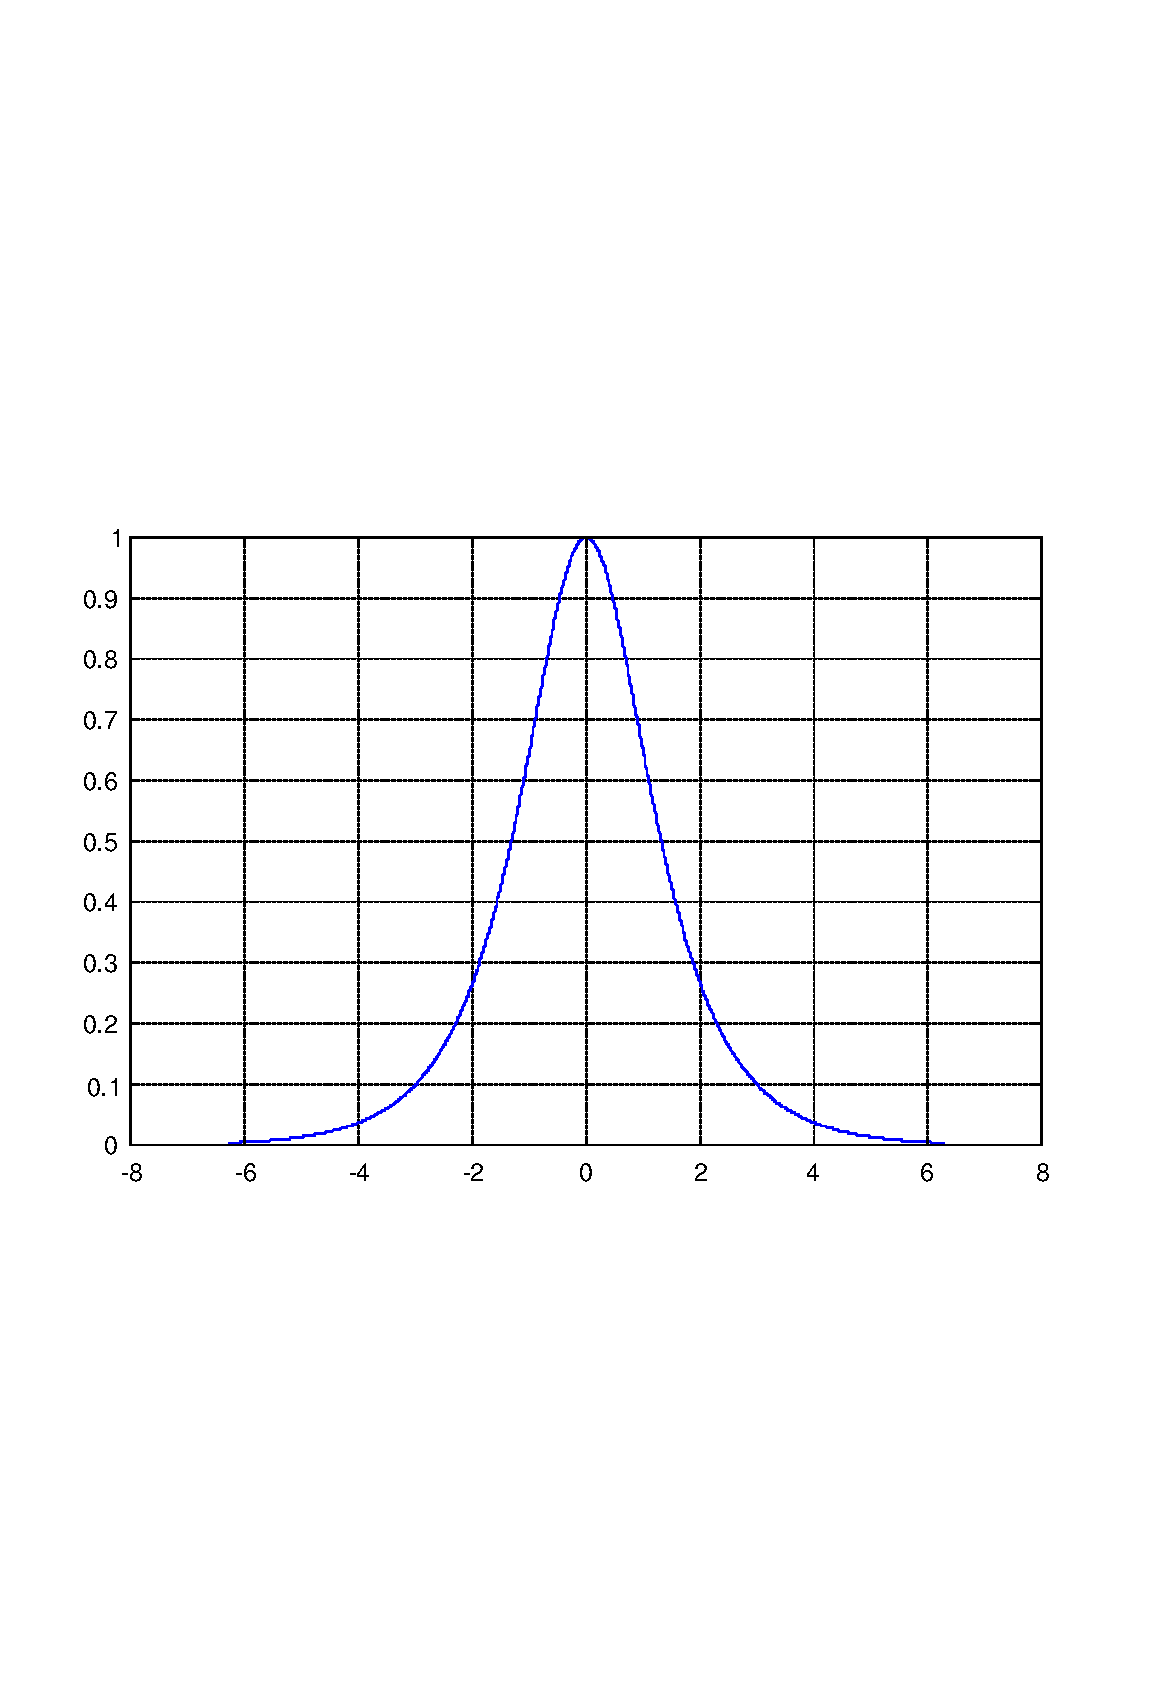
\includegraphics[width=12cm]{sechplot}
\caption{sechplot}
\end{DoxyImage}
 \hypertarget{mathfunctions_sin}{}\section{S\-I\-N Trigonometric Sine Function}\label{mathfunctions_sin}
Section\-: \hyperlink{sec_mathfunctions}{Mathematical Functions} \hypertarget{vtkwidgets_vtkxyplotwidget_Usage}{}\subsection{Usage}\label{vtkwidgets_vtkxyplotwidget_Usage}
Computes the {\ttfamily sin} function for its argument. The general syntax for its use is \begin{DoxyVerb}  y = sin(x)
\end{DoxyVerb}
 where {\ttfamily x} is an {\ttfamily n}-\/dimensional array of numerical type. Integer types are promoted to the {\ttfamily double} type prior to calculation of the {\ttfamily sin} function. Output {\ttfamily y} is of the same size and type as the input {\ttfamily x}, (unless {\ttfamily x} is an integer, in which case {\ttfamily y} is a {\ttfamily double} type). \hypertarget{transforms_svd_Function}{}\subsection{Internals}\label{transforms_svd_Function}
Mathematically, the {\ttfamily sin} function is defined for all real valued arguments {\ttfamily x} by the infinite summation \[ \sin x \equiv \sum_{n=1}^{\infty} \frac{(-1)^{n-1} x^{2n-1}}{(2n-1)!}. \] For complex valued arguments {\ttfamily z}, the sine is computed via \[ \sin z \equiv \sin \Re z \cosh \Im z - i \cos \Re z \sinh \Im z. \] \hypertarget{variables_struct_Example}{}\subsection{Example}\label{variables_struct_Example}
The following piece of code plots the real-\/valued {\ttfamily sin(2 pi x)} function over one period of {\ttfamily \mbox{[}0,1\mbox{]}}\-:


\begin{DoxyVerbInclude}
--> x = linspace(0,1);
--> plot(x,sin(2*pi*x))
\end{DoxyVerbInclude}


 
\begin{DoxyImage}
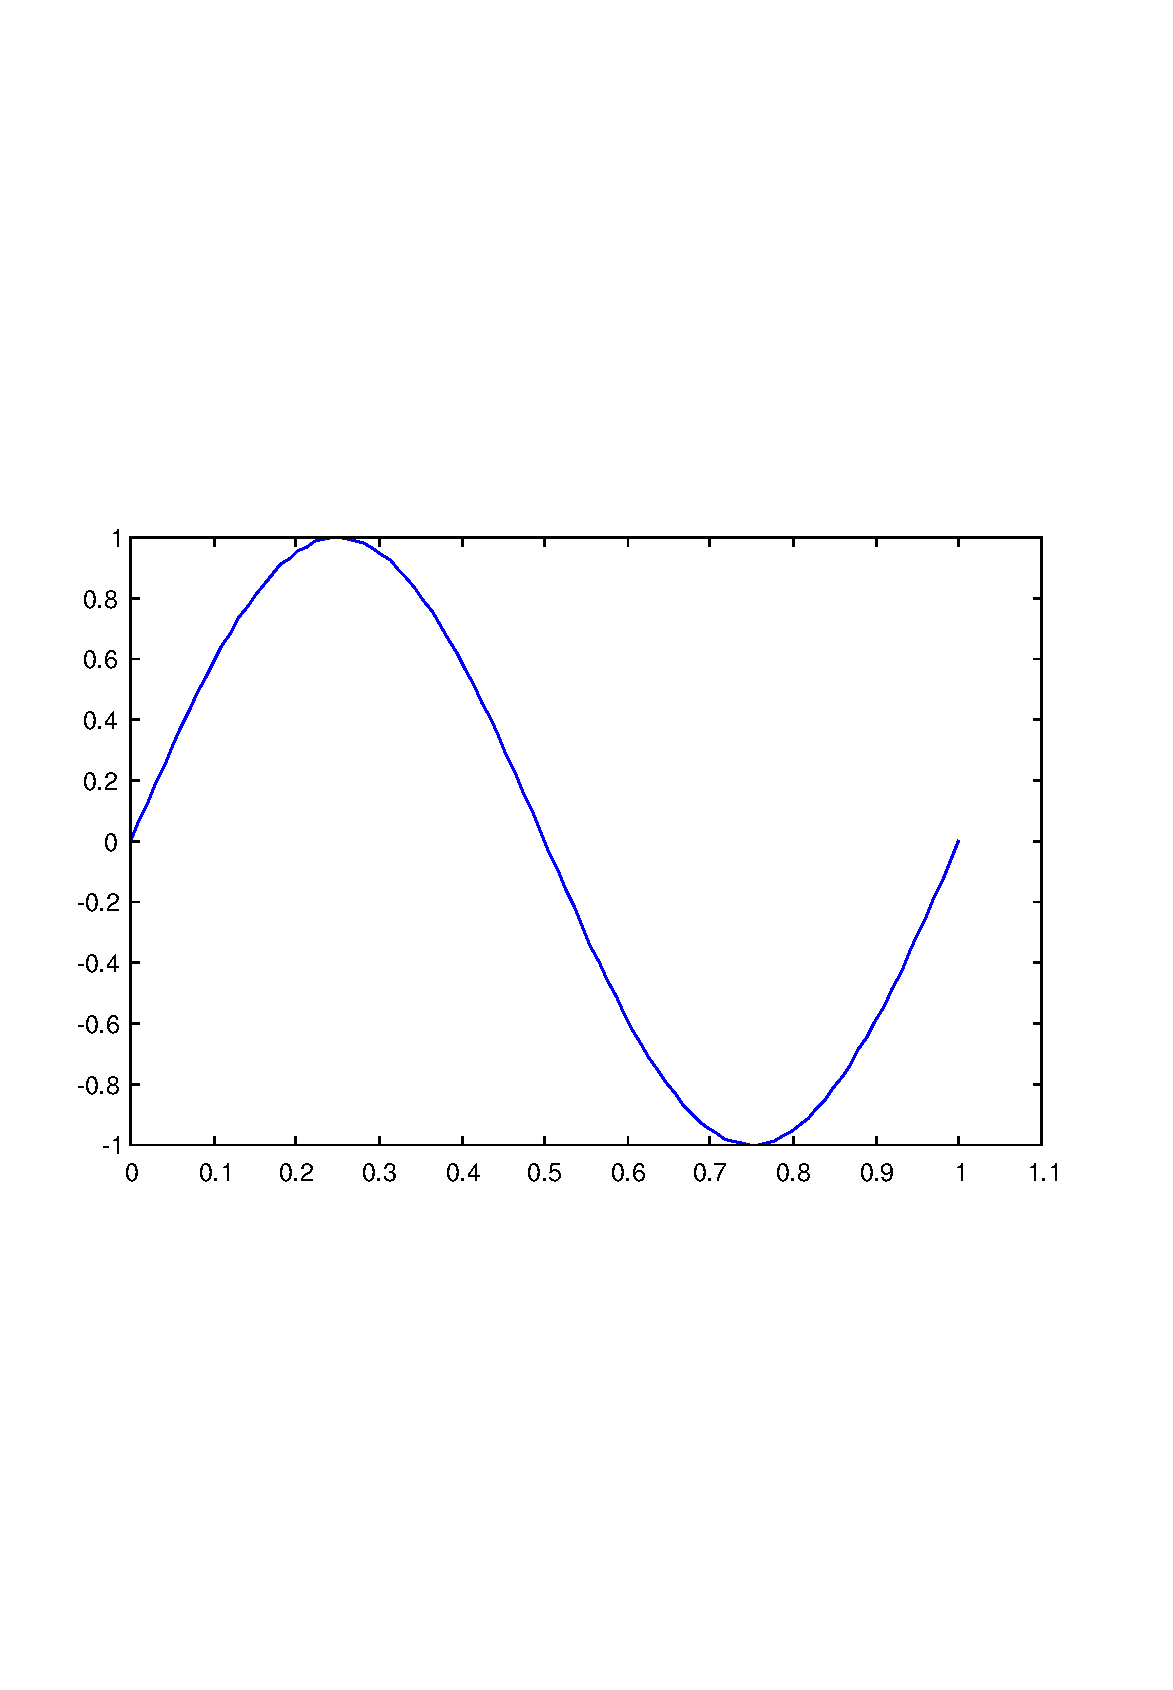
\includegraphics[width=12cm]{sinplot}
\caption{sinplot}
\end{DoxyImage}
 \hypertarget{mathfunctions_sind}{}\section{S\-I\-N\-D Sine Degrees Function}\label{mathfunctions_sind}
Section\-: \hyperlink{sec_mathfunctions}{Mathematical Functions} \hypertarget{vtkwidgets_vtkxyplotwidget_Usage}{}\subsection{Usage}\label{vtkwidgets_vtkxyplotwidget_Usage}
Computes the sine of the argument, but takes the argument in degrees instead of radians (as is the case for {\ttfamily cos}). The syntax for its use is \begin{DoxyVerb}   y = sind(x)
\end{DoxyVerb}
 \hypertarget{variables_matrix_Examples}{}\subsection{Examples}\label{variables_matrix_Examples}
The sine of 45 degrees should be {\ttfamily sqrt(2)/2}


\begin{DoxyVerbInclude}
--> sind(45)

ans = 
    0.7071 
\end{DoxyVerbInclude}


and the sine of {\ttfamily 30} degrees should be 0.\-5\-:


\begin{DoxyVerbInclude}
--> sind(30)

ans = 
    0.5000 
\end{DoxyVerbInclude}
 \hypertarget{mathfunctions_sinh}{}\section{S\-I\-N\-H Hyperbolic Sine Function}\label{mathfunctions_sinh}
Section\-: \hyperlink{sec_mathfunctions}{Mathematical Functions} \hypertarget{vtkwidgets_vtkxyplotwidget_Usage}{}\subsection{Usage}\label{vtkwidgets_vtkxyplotwidget_Usage}
Computes the hyperbolic sine of the argument. The syntax for its use is \begin{DoxyVerb}   y = sinh(x)
\end{DoxyVerb}
 \hypertarget{transforms_svd_Function}{}\subsection{Internals}\label{transforms_svd_Function}
The {\ttfamily sinh} function is computed from the formula \[ \sinh(x) = \frac{e^x-e^{-x}}{2} \] \hypertarget{variables_matrix_Examples}{}\subsection{Examples}\label{variables_matrix_Examples}
Here is a simple plot of the hyperbolic sine function


\begin{DoxyVerbInclude}
--> x = linspace(-5,5);
--> plot(x,sinh(x)); grid('on');
\end{DoxyVerbInclude}


 
\begin{DoxyImage}
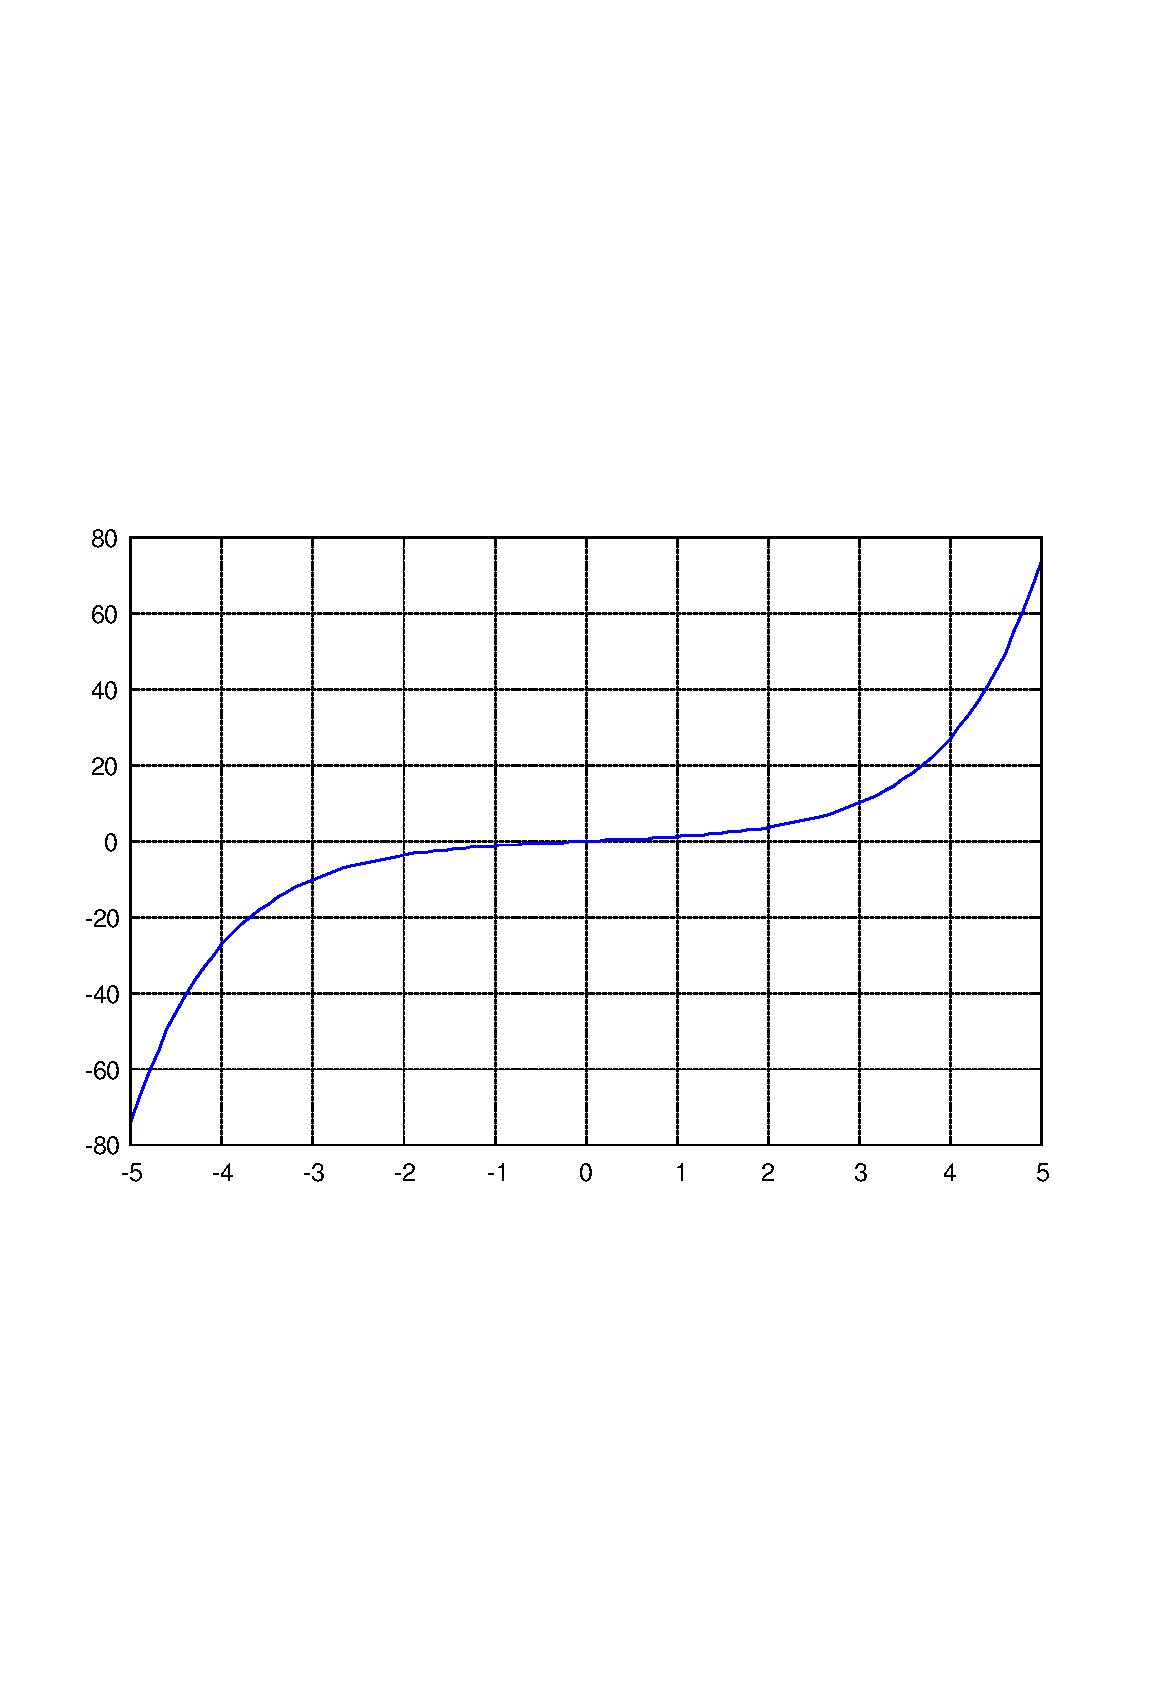
\includegraphics[width=12cm]{sinhplot}
\caption{sinhplot}
\end{DoxyImage}
 \hypertarget{mathfunctions_sqrt}{}\section{S\-Q\-R\-T Square Root of an Array}\label{mathfunctions_sqrt}
Section\-: \hyperlink{sec_mathfunctions}{Mathematical Functions} \hypertarget{vtkwidgets_vtkxyplotwidget_Usage}{}\subsection{Usage}\label{vtkwidgets_vtkxyplotwidget_Usage}
Computes the square root of the argument matrix. The general syntax for its use is \begin{DoxyVerb}   y = sqrt(x)
\end{DoxyVerb}
 where {\ttfamily x} is an N-\/dimensional numerical array. \hypertarget{variables_struct_Example}{}\subsection{Example}\label{variables_struct_Example}
Here are some examples of using {\ttfamily sqrt}


\begin{DoxyVerbInclude}
--> sqrt(9)

ans = 
 3 

--> sqrt(i)

ans = 
   0.7071 +  0.7071i 

--> sqrt(-1)

ans = 
   0.0000 +  1.0000i 

--> x = rand(4)

x = 
    0.4871    0.5309    0.3343    0.1123 
    0.7049    0.6431    0.3320    0.7799 
    0.5845    0.8331    0.9892    0.9155 
    0.5407    0.9178    0.3408    0.2274 

--> sqrt(x)

ans = 
    0.6980    0.7286    0.5782    0.3352 
    0.8396    0.8020    0.5762    0.8831 
    0.7645    0.9127    0.9946    0.9568 
    0.7354    0.9580    0.5838    0.4769 
\end{DoxyVerbInclude}
 \hypertarget{mathfunctions_tan}{}\section{T\-A\-N Trigonometric Tangent Function}\label{mathfunctions_tan}
Section\-: \hyperlink{sec_mathfunctions}{Mathematical Functions} \hypertarget{vtkwidgets_vtkxyplotwidget_Usage}{}\subsection{Usage}\label{vtkwidgets_vtkxyplotwidget_Usage}
Computes the {\ttfamily tan} function for its argument. The general syntax for its use is \begin{DoxyVerb}  y = tan(x)
\end{DoxyVerb}
 where {\ttfamily x} is an {\ttfamily n}-\/dimensional array of numerical type. Integer types are promoted to the {\ttfamily double} type prior to calculation of the {\ttfamily tan} function. Output {\ttfamily y} is of the same size and type as the input {\ttfamily x}, (unless {\ttfamily x} is an integer, in which case {\ttfamily y} is a {\ttfamily double} type). \hypertarget{transforms_svd_Function}{}\subsection{Internals}\label{transforms_svd_Function}
Mathematically, the {\ttfamily tan} function is defined for all real valued arguments {\ttfamily x} by the infinite summation \[ \tan x \equiv x + \frac{x^3}{3} + \frac{2x^5}{15} + \cdots, \] or alternately by the ratio \[ \tan x \equiv \frac{\sin x}{\cos x} \] For complex valued arguments {\ttfamily z}, the tangent is computed via \[ \tan z \equiv \frac{\sin 2 \Re z + i \sinh 2 \Im z} {\cos 2 \Re z + \cosh 2 \Im z}. \] \hypertarget{variables_struct_Example}{}\subsection{Example}\label{variables_struct_Example}
The following piece of code plots the real-\/valued {\ttfamily tan(x)} function over the interval {\ttfamily \mbox{[}-\/1,1\mbox{]}}\-:


\begin{DoxyVerbInclude}
--> t = linspace(-1,1);
--> plot(t,tan(t))
\end{DoxyVerbInclude}


 
\begin{DoxyImage}
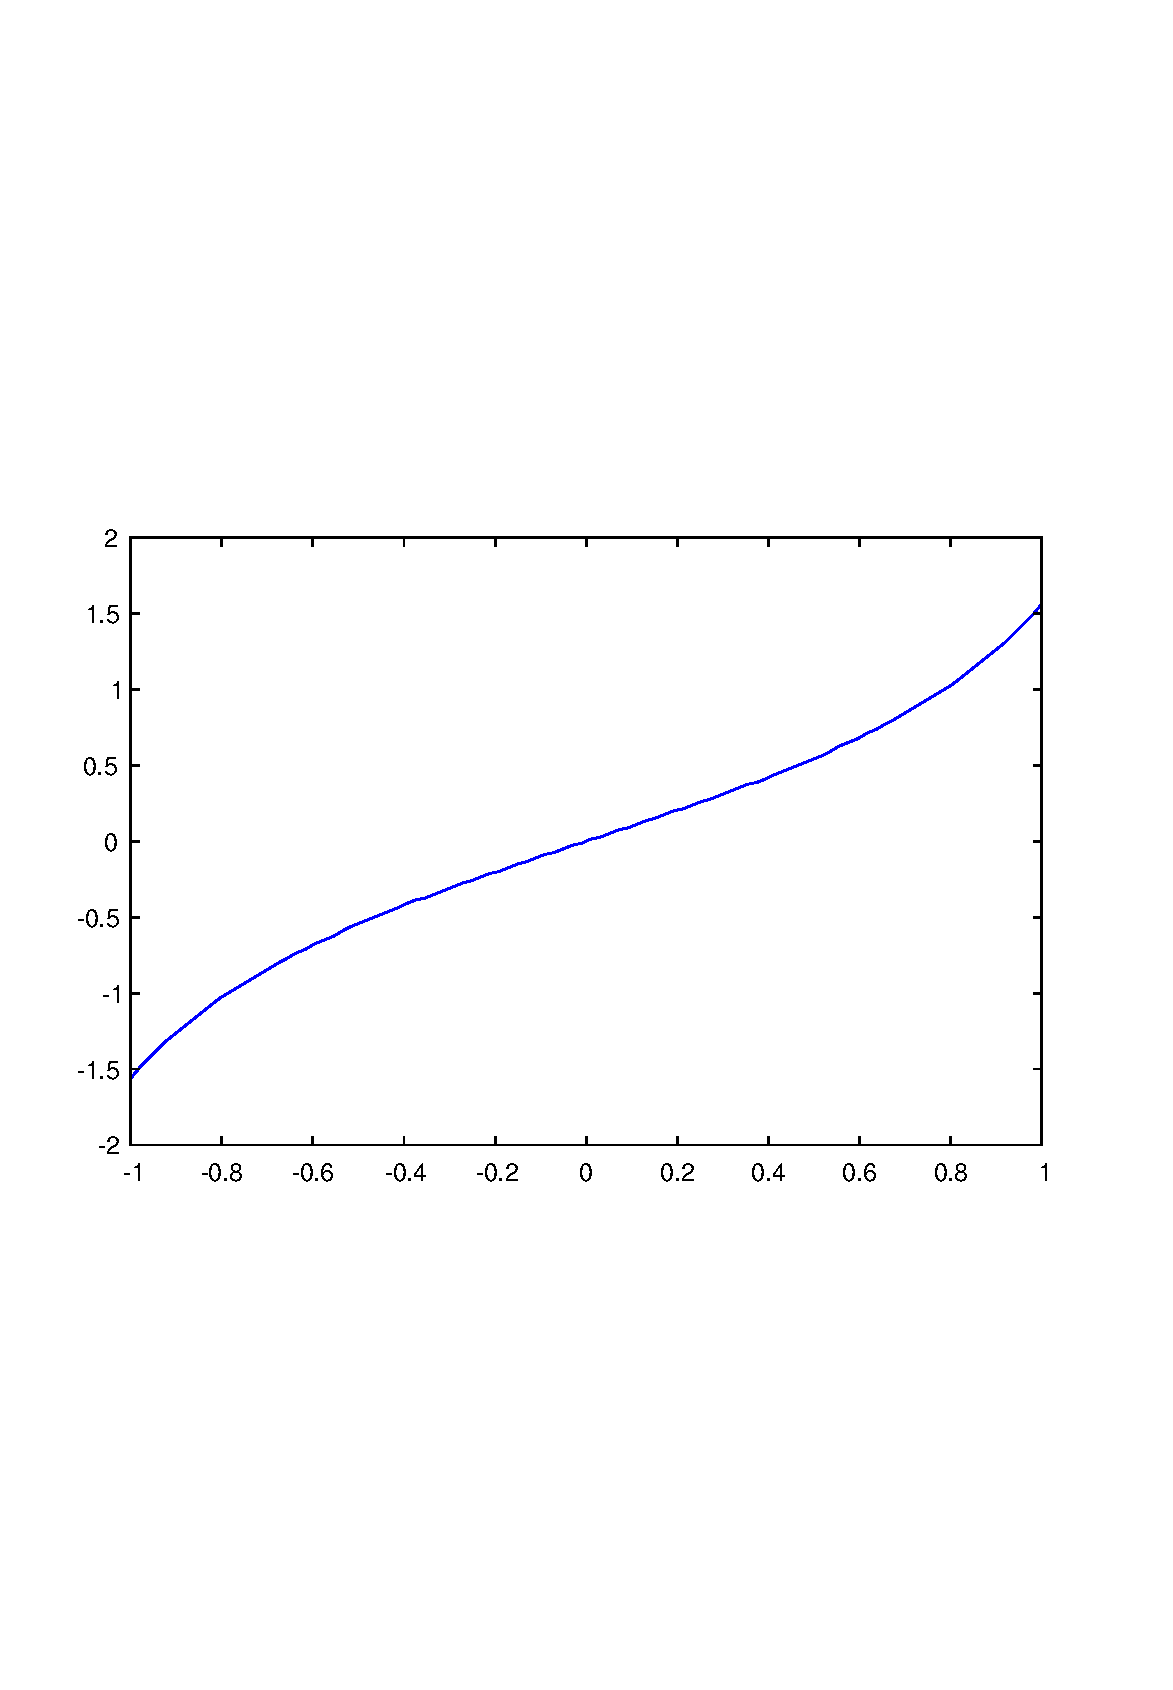
\includegraphics[width=12cm]{tanplot}
\caption{tanplot}
\end{DoxyImage}
 \hypertarget{mathfunctions_tand}{}\section{T\-A\-N\-D Tangent Degrees Function}\label{mathfunctions_tand}
Section\-: \hyperlink{sec_mathfunctions}{Mathematical Functions} \hypertarget{vtkwidgets_vtkxyplotwidget_Usage}{}\subsection{Usage}\label{vtkwidgets_vtkxyplotwidget_Usage}
Computes the tangent of the argument, but takes the argument in degrees instead of radians (as is the case for {\ttfamily cos}). The syntax for its use is \begin{DoxyVerb}   y = tand(x)
\end{DoxyVerb}
 \hypertarget{variables_matrix_Examples}{}\subsection{Examples}\label{variables_matrix_Examples}
The tangent of 45 degrees should be {\ttfamily 1}


\begin{DoxyVerbInclude}
--> tand(45)

ans = 
    1.0000 
\end{DoxyVerbInclude}
 \hypertarget{mathfunctions_tanh}{}\section{T\-A\-N\-H Hyperbolic Tangent Function}\label{mathfunctions_tanh}
Section\-: \hyperlink{sec_mathfunctions}{Mathematical Functions} \hypertarget{vtkwidgets_vtkxyplotwidget_Usage}{}\subsection{Usage}\label{vtkwidgets_vtkxyplotwidget_Usage}
Computes the hyperbolic tangent of the argument. The syntax for its use is \begin{DoxyVerb}   y = tanh(x)
\end{DoxyVerb}
 \hypertarget{transforms_svd_Function}{}\subsection{Internals}\label{transforms_svd_Function}
The {\ttfamily tanh} function is computed from the formula \[ \tanh(x) = \frac{\sinh(x)}{\cosh(x)} \] \hypertarget{variables_matrix_Examples}{}\subsection{Examples}\label{variables_matrix_Examples}
Here is a simple plot of the hyperbolic tangent function


\begin{DoxyVerbInclude}
--> x = linspace(-5,5);
--> plot(x,tanh(x)); grid('on');
\end{DoxyVerbInclude}


 
\begin{DoxyImage}
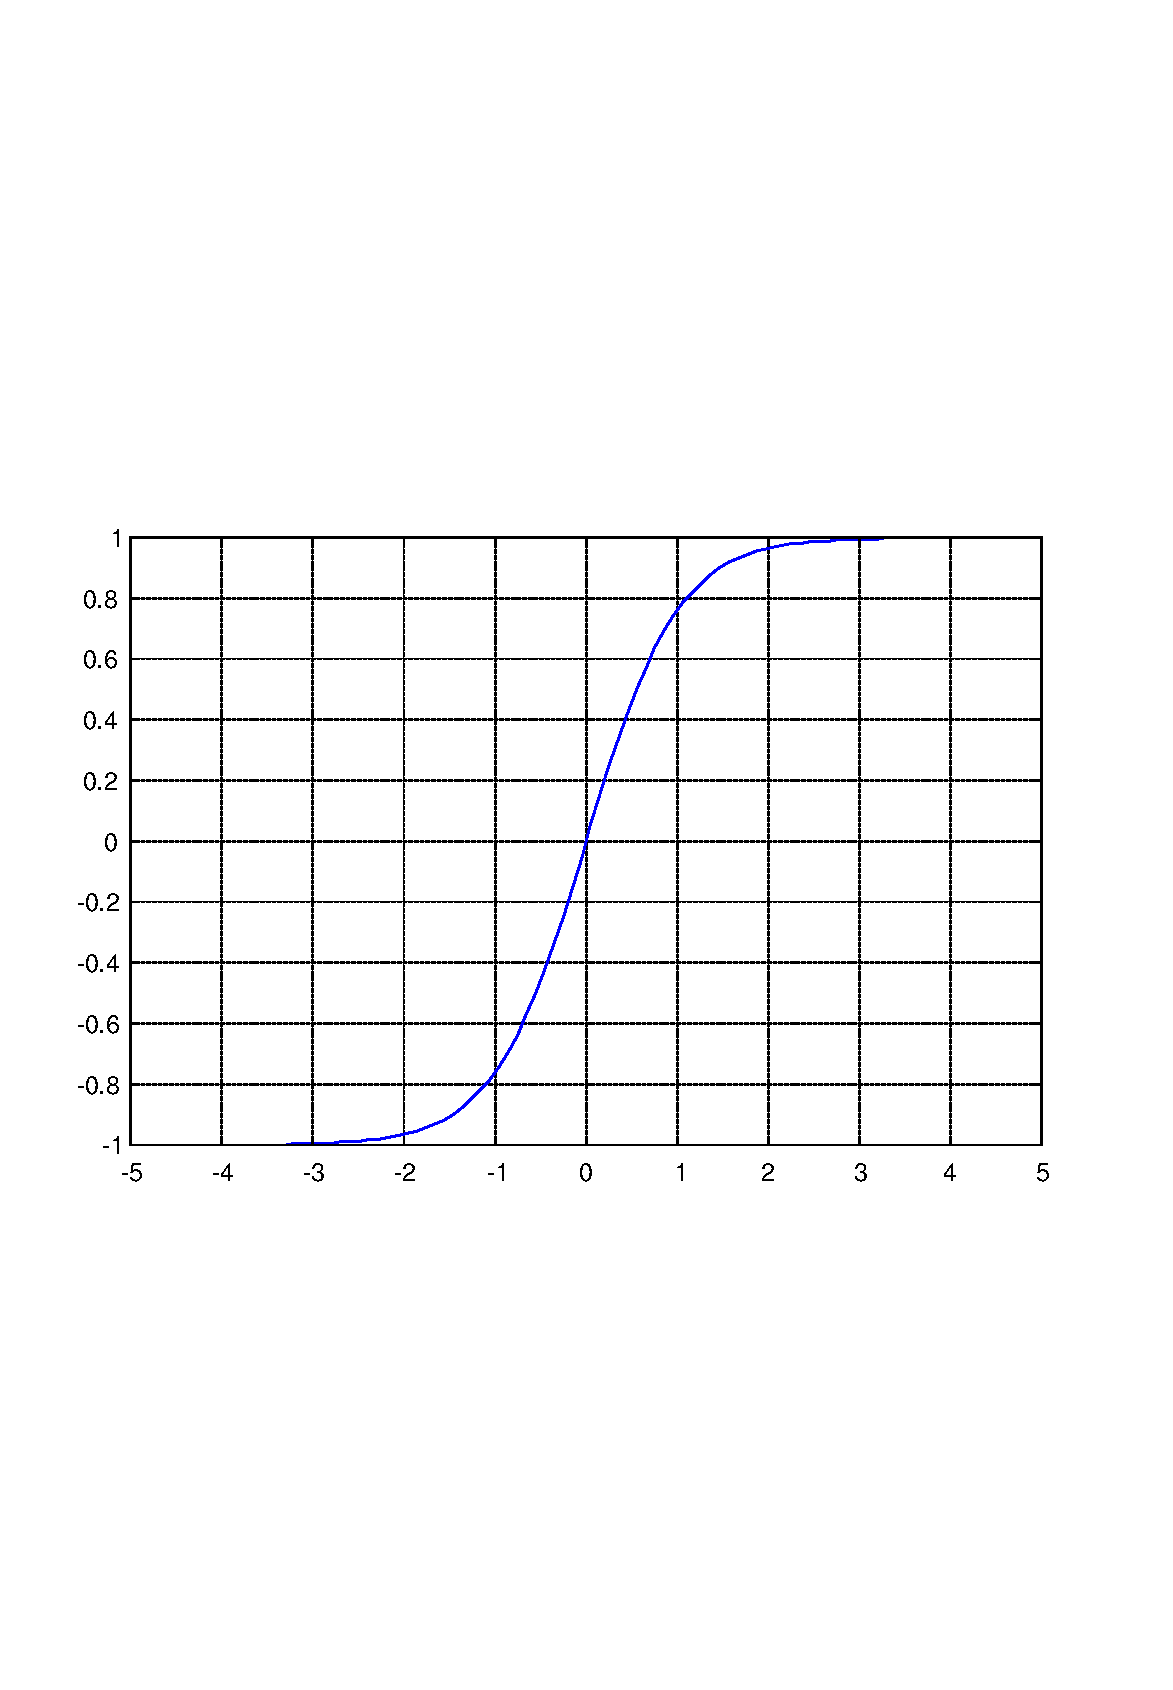
\includegraphics[width=12cm]{tanhplot}
\caption{tanhplot}
\end{DoxyImage}
 